\documentclass[a4paper,11pt]{ltjsarticle}

% ========== package ========== %
% --- 数式環境 --- %
\usepackage{amsmath}
\usepackage{amssymb}
\usepackage{mathtools}
% --- 数式環境 END --- %
% ブラケット
\usepackage{braket}
% ベクトルの太文字
\usepackage{bm}
% 添え字左右上下 \fourIdx{左上}{左下}{右上}{右下}{ベース} で使う．Iは大文字
\usepackage{fouridx}
% 色
\usepackage{color}
% 余白指定
\usepackage{geometry}
% --- ページ内リンク --- %
\usepackage{hyperref}
\hypersetup{colorlinks=true,linkcolor=blue}
% --- ページ内リンク END --- %
% 花文字
\usepackage{mathrsfs}
% 画像
\usepackage{graphicx}
% tcolorbox
\usepackage{tcolorbox}
% appendix
\usepackage{appendix}
% --- 参考文献 --- %
\usepackage{etoolbox}
\usepackage{fontspec} % fontspecは読み込んでOKですが、設定順序に注意が必要です
%% --- 参考文献フォント --- %%
  \IfFontExistsTF{Times New Roman}{
    \newfontfamily\bibfontface{Times New Roman}
  }{
    \newfontfamily\bibfontface{FreeSerif} % 代替フォント
  }
%% --- 参考文献フォント END --- %%
%% --- 参考文献リンク位置 --- %%
  \BeforeBeginEnvironment{thebibliography}{%
    \phantomsection
    \addcontentsline{toc}{section}{参考文献}
  }
  \AtBeginEnvironment{thebibliography}{%
    \normalfont\bibfontface
  }
%% --- 参考文献のリンク位置 --- %%
% --- 参考文献 END --- %
% ========== package END ========== %

% ========== newcommand ========== %
% --- セクションから目次へのリンク --- %
\newcommand{\sectionlink}[1]{\section[#1]{\hyperlink{toc}{#1}}}
\newcommand{\subsectionlink}[1]{\subsection[#1]{\hyperlink{toc}{#1}}}
% セクション番号リンク
\makeatletter
\renewcommand{\@seccntformat}[1]{%
  \protect\hyperlink{toc}{\csname the#1\endcsname}\quad
}
\makeatother

\numberwithin{equation}{section}
% ==========- newcommand END ========== %
\allowdisplaybreaks
%===========================================================
% --- タイトル --- %
%===========================================================
\geometry{left=25mm, right=25mm, top=30mm, bottom=30mm}
\title{\bfseries インフレーションの有効場理論における散逸効果\\[0.5em]
\large Dissipative effects in the Effective Field Theory of Inflation\\[0.4em]
\normalsize \href{https://arxiv.org/pdf/1109.4192v2}{arXiv:1109.4192v2 [hep-th]}}
\author{\parbox{0.96\textwidth}{\centering
Diana L\'opez Nacir$^{1}$, Rafael A. Porto$^{2,3}$,\\
Leonardo Senatore$^{4,5}$, Matias Zaldarriaga$^{2}$\\[0.8em]
\small
$^1$Departamento de F\'isica, Facultad de Ciencias Exactas y Naturales,\\
UBA and IFIBA, CONICET. Ciudad Universitaria,\\
Pabell\'on 1, 1428, Buenos Aires, Argentina.\\[0.3em]
$^2$School of Natural Sciences, Institute for Advanced Study,\\
Einstein Drive, Princeton, NJ 08540, USA\\[0.3em]
$^3$Department of Physics \& ISCAP, Columbia University,\\
New York, NY 10027, USA\\[0.3em]
$^4$Stanford Institute for Theoretical Physics, Stanford University,\\
Stanford, CA 94305\\[0.3em]
$^5$KIPAC, Stanford University \& SLAC, Stanford, CA 94305
}}
\date{2012年1月18日（原文 v2）}

%===========================================================
% --- 以下本文 --- %
%===========================================================

% Original-source mathematics macros; template class, packages and geometry retained.
\newcommand{\beq}{\begin{equation}}
\newcommand{\eeq}{\end{equation}}
\newcommand{\bea}{\begin{eqnarray}}
\newcommand{\eea}{\end{eqnarray}}
\newcommand{\bit}{\begin{itemize}}
\newcommand{\eit}{\end{itemize}}
\newcommand{\im}{\item}
\newcommand{\nn}{\nonumber}
\newcommand{\bim}{\subitem}
\newcommand{\be}{\begin{equation}}
\newcommand{\ee}{\end{equation}}
\newcommand{\lp}{\left(}
\newcommand{\rp}{\right)}
\newcommand{\lb}{\left[}
\newcommand{\rb}{\right]}
\newcommand{\ber}{\begin{eqnarray}}
\newcommand{\eer}{\end{eqnarray}}
\newcommand{\beal}{\begin{align}}
\newcommand{\eal}{\end{align}}
\newcommand{\bes}{\begin{split}}
\newcommand{\es}{\end{split}}
\newcommand{\om}{\omega}
\newcommand{\calo}{{\cal O}}
\newcommand{\calL}{{\cal L}}
\newcommand{\bphi}{{\bar\phi}}
\newcommand{\bcalo}{{\bar\calo}}

\graphicspath{{figures/}}
% Retain the template's bibliography font and interpret TeX quotation marks.
\AtBeginEnvironment{thebibliography}{\addfontfeatures{Ligatures=TeX}}
% Preserve the original equation numbers (1--212, A1, B1, ...).
\counterwithout{equation}{section}
\renewcommand{\theequation}{\arabic{equation}}
\appto\appendix{\renewcommand{\thesection}{\Alph{section}}\numberwithin{equation}{section}\renewcommand{\theequation}{\Alph{section}\arabic{equation}}\renewcommand{\thesubsection}{\arabic{subsection}}}
\hypersetup{pdftitle={インフレーションの有効場理論における散逸効果 — arXiv:1109.4192v2},pdfauthor={Diana López Nacir, Rafael A. Porto, Leonardo Senatore, Matias Zaldarriaga}}
\begin{document}
\maketitle
\begin{abstract}
単一の時計によるインフレーションの有効場理論を、散逸効果を含むように一般化する。ユニタリーゲージを用い、時間依存する空間微分同相変換の下での不変性のみを制約とする有効作用に、複合演算子の集合 $\calo_{\mu\nu\ldots}$ を結合させる。散逸を担う自由度が後期の密度摂動には寄与しない状況に限定する。このとき摂動の力学は「摩擦」項と雑音項の出現によって変化する。これらの複合演算子のGreen関数に一定の局所性を仮定すると、大きな摩擦項 $\gamma\gg H$ によって特徴づけられる領域が存在し、そこでは $\zeta$ の相関関数が雑音に支配され、パワースペクトルが大幅に増強され得ることを示す。また、広い種類の模型について3点関数 $\langle\zeta\zeta\zeta\rangle$ を計算し、どのような条件で大きな摩擦が非Gaussian性を増大させるかを論じる。とくに、本論文の仮定の下では、強い散逸と、対称性を非線形に実現するという要請とを合わせると、$|f_{\rm NL}|\sim\frac{\gamma}{c_s^2H}\gg1$ が導かれることを示す。典型例として、局所的な応答関数をもつ「トラップ型インフレーション」シナリオの変種を詳しく調べ、本論文の有効理論とのマッチングを行う。ここで述べるような、インフレーション中の散逸効果を取り入れることで生じる一般的な特徴が検出されれば、初期宇宙の力学に関する知見が得られ、インフレーション模型のパラメータ空間も広がるであろう。
\end{abstract}
\clearpage
\hypertarget{toc}{}
\tableofcontents
\clearpage
% Establish original reference order, including grouped works.
\nocite{iraeft,
joeeft,
nrgr1,
nrgr1p,
radgo,
nrgr2,
nrgr2p,
nrgr2p2,
nrgr2p2__2,
nrgr2p2__3,
nrgr2p2__4,
andi,
foffa,
eftrev,
eftrev__2,
eftfluid,
eft1,
Cheung:2007sv,
Senatore:2009gt,
Senatore:2009cf,
Senatore:2010jy,
Creminelli:2006xe,
Bartolo:2010bj,
Bartolo:2010di,
dan2,
strongc,
dan2new,
peskin,
ben,
multieft,
trapped,
beauty,
calzetta,
dis1,
dis2,
hydro,
efthydro,
efthydro__2,
berera1,
berera1__2,
berera2,
warm,
warm__2,
warm__3,
weiss,
Zhang,
Fetter,
radre,
radre__2,
memory,
gel,
Komatsu:2010fb,
consist,
creminelli11,
warmf33,
berera11,
reheating,
bastero,
bueno,
linde,
hall,
warmf1,
gwssz,
forster,
weinberg}

\sectionlink{序論と主な結果}\label{warm}

有効場理論（EFT）という考え方は、標準模型から物性系に至るまで、理論物理学の礎の一つである\cite{iraeft,joeeft}。近年、EFTの考え方は重力物理学の分野でも勢いを増している。例えば、文献\cite{nrgr1,nrgr1p,radgo}では、合体する連星系の力学を高精度で解くためにEFTの手法が導入されている\cite{nrgr2,nrgr2p,nrgr2p2,andi,foffa,eftrev}。また、宇宙論的摂動を研究するためのEFTの枠組みが文献\cite{eftfluid}で提案されている。

単一場（単一時計）模型に対するインフレーションのEFTは、文献\cite{eft1, Cheung:2007sv, Senatore:2009gt, Senatore:2009cf, Senatore:2010jy, Creminelli:2006xe, Bartolo:2010bj, Bartolo:2010di,dan2,strongc,dan2new}で構築された。その出発点は、時間に依存する空間微分同相変換の下で不変であることだけを要求した、ユニタリーゲージでの作用である。このゲージでは、揺らぐ自由度はすべて計量に組み込まれている。この方法の利点は、低エネルギー（長距離）の自由度から構成され、理論の対称性だけによって制約されるLagrangianに現れる（「高次元」）演算子の係数の組を用いて、インフレーションのあらゆる可能な観測的特徴をパラメーター化できることである。EFTでは、インフレーションを駆動する基本的な自由度について何も仮定せずに、近似的なde Sitter背景の周りの揺らぎを記述できる\footnote{背景を生み出す基礎理論について疑問を抱くかもしれない。しかし、インフレーションの枠組みをひとたび受け入れれば、最終的に観測によって直接検証されるのは揺らぎの理論である。}。その基本的な自由度は、強結合であってもよい。
この目的には、優先される時間スライスの存在によって破れた時間微分同相不変性を、St\"uckelberg場$\pi$によって回復すると便利である。この場は、時間の再パラメーター化を非線形に実現するGoldstoneボソンである。

$\pi$場の導入には、きわめて有用な二つの重要な帰結がある。第一に、十分高いエネルギー（$E \gg \sqrt{\epsilon} H$）では、Goldstoneボソンが物理的なスカラーモード（$\zeta\simeq-H\pi$）、すなわちユニタリーゲージにおける「縦モード」のすべての情報を担う\footnote{これはゲージ理論で起こることと類似している。例えば、縦偏極した$WW$（または$Z$）の散乱では、十分高いエネルギー$E \gg m_W$において、その振幅を対応するGoldstoneボソン（$W$と$Z$に「食べられた」もの）を含む過程から求められる（「等価定理」）\cite{peskin, ben}。}。第二に、重力相互作用が誘起するすべての効果を無視できる極限（分離極限、すなわち$\epsilon \to 0$）が存在する\footnote{これは、対称性の破れのスケール$v$を固定したままゲージ結合$g$をゼロにすることにも相当する。本論文の場合には、$M_p^2|\dot H|$を有限に保ちながら$M_p\to \infty$とすることである。}。この二つの事実により、対称性によって相互作用が定まるGoldstoneボソンの理論に集中でき、計算が大幅に簡単になる。

最近、文献\cite{multieft}では、新しい（軽い）自由度を含む多場インフレーションのEFTが導入された。多場インフレーションは単一場模型の信号を再現できる一方、新しい信号を生み出すこともできる。そのような信号の特定の形状が検出されれば、両者を区別するだけでなく、多場シナリオの異なる実現を区別できる可能性もある。文献\cite{multieft}の著者らは、追加自由度（ADOF）が全曲率摂動（あるいは等曲率摂動）に直接影響する場合に注目した。これは例えば、追加の場が再加熱の時刻、したがってインフレーションの継続時間を変える場合や、再加熱期のプラズマの組成に影響する場合に起こる。そのため、文献\cite{multieft}で考察された場は、スケール不変な摂動を獲得する軽いスカラー場であった。

本論文でも、Goldstoneボソン以外のADOFが励起される状況を考える。しかし、文献\cite{multieft}の模型とは異なり、この追加セクターがインフレーションの継続時間やプラズマの組成に直接影響せず、観測するモードが地平線を横切る頃またはそれ以前に時計へ直接結合することで、インフレーションの力学を変える場合に注目する。これには例えば「トラップ型インフレーション」のシナリオ\cite{trapped}が含まれる。このシナリオでは、粒子生成がインフラトン$\phi$の発展を変える一方、希釈のため、晩期の密度揺らぎへの直接の寄与は無視できる。

一般に、これらの新しい粒子は背景のエネルギー運動量テンソルに寄与する。そのため、{\it 真の}Goldstoneボソンは、インフレーションの物理を一意に支配すると仮定した物理的な時計だけでなく、これらのADOFの揺らぎに依存する成分も含む。観測される密度揺らぎをその摂動が支配する成分を取り出すため、ここではこのGoldstoneボソン、すなわち二次のLagrangianが背景によって一意に決まる場を用いない。代わりに、インフレーションの終わりを決める時計の揺らぎ（例えば文献\cite{trapped}の模型におけるインフラトン$\phi$）を$\pi$と表す。この選択により、EFTの構成、とりわけ「ユニタリーゲージ」の選び方と$\pi$の全体の規格化が少し変わる。しかし、$\pi$と$\zeta$の関係、すなわち線形次数での$\zeta \simeq -H\pi$は保たれるため、こちらの方が便利である。\\

ADOFは観測量に明示的には寄与しないので、これらを積分消去し、$\pi$だけで表された有効作用を得られるように思われる。しかし、この手続きは主に二つの理由で単純ではない。第一に、ADOFの揺らぎを「外線状態」として観測しなくても、それらはインフレーション中に生成され、一般には真空状態にない。第二に、これらの揺らぎにはギャップがない可能性があり、言い換えれば、非常にソフトな（本質的にギャップのない）集団励起を許している。このため、有効作用は一つの自由度だけでは記述できず、このことは散逸につながる。散逸を有効的に記述することは本論文の目的の一つである。これは、ADOFが必ず「軽い」ことを意味するわけではない。例えば文献\cite{trapped}で示されたように、物理的な時計$\phi$が誘起するHamiltonianの時間依存性によって、Hubbleスケールに比べて重い粒子も生成されうる\footnote{トラップ型インフレーションでは、断熱条件が破れたときに粒子が生成される\cite{beauty,trapped}。}。しかし、散逸と雑音を含む、時計の摂動の力学へのそれらの影響は、より低い周波数、すなわち$\omega \simeq H$でも働き続ける。\\

散逸効果は「in-in」閉時間経路形式\cite{calzetta}を用いて調べられるが、ここでは別の枠組みを採用する。連星ブラックホール系による重力波吸収を扱うために文献\cite{dis1,dis2}で導入された散逸のEFTと同様に、ユニタリーゲージの計量を、EFTの対称性だけによって制約される一組の複合演算子$\cal O_{\mu\nu\ldots}$（スカラー、ベクトル、テンソル）に結合させることで、インフレーションのEFTに散逸効果を組み込む。したがって、散逸セクターに関するすべての情報は、パワースペクトルや非Gaussian性などの観測と照合できる一組の相関関数に符号化される。（類似の形式\cite{hydro}を用いると、文献\cite{efthydro}で構築された流体力学のEFTにおける散逸効果も記述できる。）
この方法の適用範囲は明らかに非常に広く、それゆえ完全に一般的な形で扱うのは難しい。しかし、パラメーター空間の中に、多くの簡単化が起こる物理的領域を特定できる。ここでは、ADOFによって誘起される散逸と揺らぎの時間スケールがHubble時間よりはるかに短く、記憶効果を無視できる物理的状況を考える。この条件の下では、揺らぎと散逸の効果が局所的になり、多くの可能な実現を完全に一般的な形で調べられる。本論文では、仮定を随所で詳しく明示する。\\

$\pi$の力学には、二種類の異なる寄与が入る。一つはADOFが誘起する雑音であり、もう一つは相互作用に伴う反作用、すなわち「摩擦」である。後者は$\gamma\dot\pi$という項で表される。（これは、インフレーション中にエネルギーがADOFへ散逸するという物理的事実による。）
ここでは、$\gamma$が$H$よりはるかに大きい強散逸領域に注目する。この状況では初期条件の記憶が失われ、パワースペクトルと非Gaussian性がADOFによって誘起される雑音に支配されることを示す。さらに、パワースペクトルはBunch-Davies状態の量子揺らぎに比べて大幅に増強されうる。その理由は二つある。第一に、規格化された$\pi$場（$\pi_c \equiv \sqrt{N_c}\pi$）の揺らぎの大きさはHubbleスケールより大きい。これは、揺らぎが真空によって生成されるものではないためである。また、より大きな$k/a$で凍結し、$\gamma \gg H$に対して$c_s k/a_\star = c_s k_\star \simeq \sqrt{\gamma H} \gg H$となる。第二に、規格化スケール$N_c$は、エネルギー運動量テンソルへのほかの寄与が存在しない場合にEinstein方程式が要求する値より小さくなりうる。すなわち、$N_c \leq 2 M_p^2|\dot H|/c_s^2$である。\\

インフレーションのEFT~\cite{eft1}では、時間微分同相変換の非線形な実現によって、異なる観測量（例えば$\zeta$の二点相関関数と三点相関関数）を関係づけられる。例えば、スカラー結合を考え、雑音をGaussianとすると、ユニタリーゲージで$S_{\calo g^{00}} \equiv \int \sqrt{-g}\calo g^{00}$の形をもつ項は、ADOFのない単一場インフレーションの結果\cite{eft1}に比べ、非Gaussian性の大きさを$\gamma/H$倍に増強し、$|f_{\rm NL}| \simeq \gamma/(Hc_s^2)$を与えうることを示す。文献\cite{multieft}の多場インフレーションのEFTの考え方に沿って、この分類に属する一群の模型を議論する。
一方、$S_{f\calo}\equiv \int \sqrt{-g} f(t)\calo$の形の演算子は二種類の非線形性を生む。一つは$\calo$への直接の非線形結合に由来し、もう一つは線形応答理論を超えた寄与によって誘起される。散逸の計算と非Gaussian性の計算が結びつく模型のクラスが存在することを示す。本論文で仮定するように、インフレーションを駆動する優先的な時計が存在するとき、線形応答と非線形応答は実際に関係づけられ、$|f_{\rm NL}| \simeq \gamma/(c_s^2H)$程度の非Gaussian性を生じる。

基本的な考え方は、スローロールするスカラー場$\phi$による標準的なインフレーションのシナリオで示すと、よりわかりやすいであろう。古典力学の直感からわかるように、散逸を誘起するには運動方程式（EOM）に$\dot\phi$の因子が必要である。一方、非線形に実現された一般共変性は、$\partial_t\phi \to n^\mu \partial_\mu \phi$を要求する。ここで$n^\mu$は等時刻面に直交する法線ベクトルで、$n^\mu = g^{\mu\nu}\partial_\nu \phi/\sqrt{-(\partial\phi)^2}$で与えられる。時計の摂動、すなわち$\phi \to \bphi + \delta\phi$のレベルでは、これによって散逸項$\gamma\dot{\delta\phi}$だけでなく非線形相互作用も誘起され、とりわけ適切に規格化された$\gamma (\partial_i\delta\phi)^2/\dot\bphi$という項が生じる。後者は次の程度の非Gaussian性を与える。
\beq \frac{\gamma}{\dot\bphi}\frac{(\partial_i \delta\phi)^2}{c_s^2\partial_i^2\delta\phi} \sim f_{\rm NL}\zeta \quad \to \quad |f_{\rm NL}| \sim \frac{\gamma}{c_s^2 H},\eeq
ここでは$\zeta \simeq -H\delta\phi/\dot\bphi$を用い、$c_s \leq 1$を許した。以下では、この議論をより厳密にするとともに、単一時計インフレーションのすべての模型に対して一般化する。$S_{\calo g^{00}}$と$S_{f(t)\calo}$のいずれの場合にも、素朴に予想されるとおり、$\gamma \gg H$の強散逸領域では非線形相互作用が大幅に増強されると結論される。

最後に、$\int \sqrt{-g} \calo_\mu g^{\mu0}$のようなベクトル結合は、$\pi$と$\calo_\mu$の間に非線形結合を追加せずに、大きな摩擦項を誘起しうる。しかし、この場合も模型によっては、非線形応答が上と同様に大きな非線形性を生み出す。\\

本論文の構成は次のとおりである。第\ref{warm}節の残りでは、計算の技術的細部よりも全体像に重点を置き、基本的な考え方と結果を議論する。続く第\ref{eftsup}--\ref{nongaus}節では、インフレーションの散逸を含むEFTを明示的に構成し、主張の詳細な根拠を与える。第\ref{matching}節では、重要な例であるトラップ型インフレーションの局所版についてマッチングを行う。インフレーション中に散逸効果を含めるという考え方は、温かいインフレーションの枠組み\cite{berera1,berera2,warm}でも重要な要素であり、終盤で簡単に触れる。ほかの例とより技術的な点は付録にまとめる。全体を通じて$c=\hbar=k_B=1$とし、計量の符号は空間成分を正とする規約を採用する。

\subsectionlink{準備}
一次元調和振動子に摩擦項を加えることを考えよう。記法の都合上、平衡点からの変位を$\pi(t)$と表す。運動方程式は
\beq
\label{eom1}
 \ddot \pi + \gamma\dot \pi + \omega_0^2 \pi = J,
\eeq
である。ここでは後のために、$\langle J\rangle=0$を満たす確率的な力を加えた。
よく知られているように、一見何の問題もなさそうなこの方程式は、$\calL(\pi,\dot \pi)$の形のLagrangianからは導かれない\footnote{
それでも、自由度を二重化した「in-in」形式で、散逸を担うADOFを「積分消去」した有効記述から散逸方程式が得られる模型を構成することはできる\cite{calzetta,weiss,Zhang}。本論文ではこの方法は採らない（次の小節を参照）。}。理由は単純で、エネルギーが保存しないからである。実際、
\beq
\label{eneloss}
\frac{dE}{dt} =-\gamma \dot\pi^2.
\eeq

式(\ref{eom1})は時間に局所的である。しかし、一般に$\pi$の有効運動方程式は、非局所的ないわゆる「Langevin」形式、すなわち
\beq
\ddot\pi +\omega_0^2 \pi +  \int dt' \tilde\gamma(t-t')\pi(t') = J(t).
\eeq

局所近似が可能であれば、扱いが大幅に簡単になることは明らかである。これは、上式の$\tilde\gamma(t)$を生み出すADOFについて仮定を置くことに相当する。特に、式~(\ref{eom1})の形の運動方程式を得るには、
\beq
\label{imgam}
{\rm Im} \tilde\gamma(\omega) \simeq  \gamma \omega,
\eeq
が必要であり、$\gamma$は定数である。式~(\ref{imgam})の関係は、文献では{\it Ohmic}な振る舞いと呼ばれることがある\cite{weiss}。付録\ref{app0}でいくつかの例を示す。\\

実際には、式(\ref{imgam})が任意に高い周波数まで成立するとは考えられない。現象論的ではあるが、より現実的な方法はDrude模型によって与えられ、式(\ref{imgam})を次の式で置き換える\cite{weiss}。
\beq
\label{imdrude}
{\rm Im} \tilde\gamma_D(\omega) = \gamma \omega \left(1+ \omega^2/\omega_D^2\right)^{-1},
\eeq
ここで$\omega_D$はカットオフとして働く。この場合、$\tau_D \sim \omega_D^{-1}$程度の記憶時間が存在し、次の指数減衰が生じる。\beq \gamma_D(t) \sim \Theta(t)\gamma_D
\frac{e^{-t/\tau_D}}{\tau_D}.\label{drude}\eeq

ADOFの物理についての仮定に頼る代わりに、よく知られた定理を用いて雑音とGreen関数の性質を関係づけられる場合がある。例えば、雑音が次の条件を満たすと仮定する。
\bea
\langle J(t) \rangle &=& 0 \\
\langle J(t)J(t') \rangle &\simeq& \nu_J \delta(t-t') \label{whiten},
\eea
ここで$\nu_J$は定数である。これは例えば、「環境」、すなわち散逸を担うADOFが十分高い温度$T$に置かれた場合に成り立つ。このとき、揺動散逸（FD）定理\cite{calzetta, weiss}を用いると、
 \beq
 \label{fdth}
 {\rm Im} \tilde\gamma(\omega) \simeq  \frac{\nu_J}{T} \omega
\eeq
を示せる。ただし、摂動を加えた後に十分速く平衡化するものと仮定する。言い換えれば、$\nu_J \simeq \gamma T.$である。このシナリオでは運動方程式が局所的になり、記憶効果は消失する。\\

できるだけ簡単に扱うため、局所近似が適用できる状況を調べる。後で具体例をいくつか議論するが、EFTのレベルでは、ADOFの基礎的な力学について特定の模型を採用しない。次に、本手法の基本的な考え方を導入する。


\subsectionlink{\texorpdfstring{$\cal O$の役割}{Oの役割}}\label{storyo}

次に、Lagrangian ${\cal L}_\pi$をもつ力学系の小さな長波長摂動を記述する$\pi$の理論があるという一般的な状況を考える。文献\cite{dis1,dis2}に従い、散逸を含めるために$\pi$を複合演算子$\cal O$へ次のように結合させる。
\beq
\label{calopi}
S_{\rm int} =- \int d^4x \calo(x)\pi(x).
\eeq
シフト対称性$\pi \to \pi +c$が存在する場合、相互作用は
\beq
\label{tcalop}
\tilde S_{\rm int} =\int d^4 x \tilde\calo(x)\dot\pi(x),
\eeq
という形を取る。これは、$\calo \to \dot{\tilde\calo}$と置き換えれば、式(\ref{calopi})と同様に記述できる。\\

$S_{\rm int}$を加えることで、$\calo$で表される散逸セクターとの相互作用に対する系の応答を、
完全に一般的な形で調べられる。この方法の長所は、原理的には強結合セクターを表しうる$\calo$の力学に特定の表現を仮定する必要がなく、式(\ref{calopi})のような相互作用が、$\pi$によって記述される長距離の物理の対称性を満たすことだけを確かめればよい点にある\cite{dis1,dis2}。\\
 
ここで、$\bar\calo$を$\calo$の背景期待値として、演算子$\delta\calo\equiv \calo-\bar\calo$を定義する。次に、$\delta\calo$を模式的に二つの部分へ分解する。
\beq
\delta\calo = \delta\calo_S(x) + \delta\calo_R(x),
\eeq
$\delta\calo_S(x)$は$\pi$が存在しない場合の$\calo(x)$の確率的な部分を表し、
$\delta\calo_R(x)$は相互作用を通じた$\pi$の揺らぎへの応答として生じる、$\calo$の期待値の変化に対応する。まず線形応答理論の範囲で$\delta\calo_R(x)$を計算する。この際、$\pi$は、演算子$\calo$に対応する自由度の力学を乱す外部の「力」として働く。（応答理論の入門的説明については、
例えば文献\cite{Fetter}を参照。）すなわち、
\beq
\label{dret0}
\delta\calo_R(x) =  -\int d^4y G_{\rm ret}^\calo(x,y)\pi(y),
\eeq
ここで、
\beq
\label{dret}
G_{\rm ret}^\calo(x,y) = i\langle[\delta\calo(x),\delta\calo(y)]\rangle \theta(t_x-t_y).
\eeq

ADOFがない場合に$\cal L_\pi$から導かれる線形化された運動方程式を$D_\pi \pi=0$と表すと、式(\ref{calopi})を加えることで
\beq
D_\pi \pi =- \calo  + O(\pi^2).
\eeq

$\calo$について解くと、
\beq
\label{dpig}
D_\pi \pi -  \int d^4y G_{\rm ret}^\calo(x-y)\pi(y) = -\delta\calo_S + O(\pi^2),
\eeq
を得る。Fourier空間では、
\beq
\left(D_\pi({\bf q},\omega)- G_{\rm ret}^\calo({\bf q},\omega)\right) \pi_q(\omega) =-\delta\calo_S({\bf q},\omega) + \ldots.
\eeq

上式の$D_\pi({\bf q},\omega)$は解析関数だが、$G_{\rm ret}^\calo({\bf q},\omega)$については必ずしもそうとは限らない。しかし、広い周波数範囲で、Green関数が誘起する力学に対して局所近似を用いることができ、補正は$({\bf q}/M_\calo, \omega/\Gamma_\calo)$程度であると仮定する。ここで$M_\calo,\Gamma_\calo$は、非局所性が無視できなくなり始める典型的なスケールである。インフレーションの場合を調べる際に、この点をより厳密に述べる。いずれにしても、式(\ref{eom1})のような方程式を再現するには、次が必要であることは明らかである\footnote{予想されるように、散逸はFourier空間のGreen関数の虚部に関係する。これは光学定理としても知られる。付録\ref{appA}を参照。}。
\beq
\label{expG}
{\rm Im} G_{\rm ret}^\calo (\omega,{\bf q}) \simeq {\rm Im} G_{\rm ret}^\calo (\omega,{\bf 0}) \simeq  \gamma \omega,
\eeq
これは$\omega>0$に対する式であり、$J \equiv -\delta\calo_S$である。微分展開は$\omega\lesssim \Gamma_{\cal O}$で考えられることによって正当化されるが、Taylor展開がどの次数から始まるかは紫外（UV）の物理についての仮定である。（Green関数の虚部は$\omega$の奇関数でなければならないため、これは解析的な項の最低次数である。）

虚部とは異なり、Green関数の実部は$\omega$の偶関数なので、$\omega \to 0$で消える必要はない\footnote{さらに、Green関数$G^\calo_{\rm ret}(\omega,{\bf q})$の実部は、${\bf q}$の二次の項を通じて音速にも寄与しうる。}。これは$\pi$、したがって$\zeta$に質量を与え、地平線外で$\zeta$が時間発展することにつながる。これを禁止する原理はないが、もしそうであれば、ADOFが晩期の曲率摂動へ影響することになる。この影響は、本論文の主な仮定によれば無視できなければならない。そこで本論文では、ADOFが$\pi$自体の値には感応せず、$\pi$の微分のみに感応する状況を考える。これには、応答のレベルで有効的なシフト対称性が必要である。（例えば文献\cite{trapped}の模型はこの場合に当たり、ADOFの生成は時間依存する背景による断熱性の破れ\cite{beauty}と結びつき、ADOFの揺らぎは$\pi$の微分に関係する。）例えばインフレーションがスカラー場$\phi$によって駆動される場合、原理的には$\calo$演算子の応答が$\phi$と強い非線形な関係をもちうる。また、$\pi$のGreen関数も、$\phi$と$\calo$の両方を含むLagrangianの結合定数に非線形に依存しうる。実際、この段階ではシフト対称性自体が存在しない可能性もある。このため、$\omega\rightarrow 0$でGreen関数の実部が消える場合を「創発的シフト対称性」と呼ぶ。この現象の例を、第~\ref{localtrap}節でトラップ型インフレーション模型~\cite{trapped}の簡略版を議論する際に示す。\\

原理的には、ADOFについて特定のUV模型があれば、厳密なGreen関数を計算し、EFTから導かれたものと比較できる。これはEFTでは典型的な手続きであり、しばしば{\it マッチング}と呼ばれる\cite{iraeft}。後の第~\ref{matching}節で具体的な模型を調べる際に、このマッチング手続きを実行する。（付録\ref{appB}と\ref{mag00}も参照。）それでも、$\calo$の明示的な記述がなくても（それはかなり複雑かもしれない）、式(\ref{dret})型のGreen関数を用い、$\gamma$を自由パラメーターとして残した式~(\ref{expG})の近似の下で$\pi$の力学を調べられることが、EFTの方法の要点である。\\

$\gamma\dot\pi$という局所的な散逸力学の条件は、
\beq
\label{tildG}
{\rm Im} \tilde G_{\rm ret}^\calo (\omega) \sim 1/\omega,
\eeq
を、式(\ref{tcalop})の演算子$\tilde\calo$に要求することに注意しよう。この振る舞いは、Green関数の基本的な解析的性質により、$\omega\simeq 0$の近傍では許されない。それでも、中間周波数$\mu_\calo \ll \omega \ll \Gamma_{\calo}$では式(\ref{tildG})が成立し、非常に低い周波数ではGreen関数が解析的になる状況は考えられる。ここで$\mu_\calo, \Gamma_\calo$は$\calo$の応答関数に関連する量である。問題となるエネルギースケールはADOFセクターの典型的なスケールより小さく、その典型的スケールを$\Gamma_\calo$程度と仮定している。そのため、このような振る舞いが生じるには、Green関数が$\Gamma_\calo$に比べて異常に低い質量スケールをもつ必要がある。これはおそらく、有効理論における調整の徴候である\footnote{付録\ref{mag00}では、調整によって式(\ref{tildG})のスケーリング、具体的には
\beq
\omega^2{\rm Im}{\tilde G}_{\rm ret}^{\calo}(\omega) \simeq \gamma \frac{\omega^3}{\omega^2+\mu_\calo^2} + O(\omega/\Gamma_\calo) \simeq  \gamma\omega + O(\mu_\calo/\omega, \omega/\Gamma_\calo)
\eeq
を$\mu_\calo \ll \omega \ll \Gamma_{\calo}$に対して得られることを示す。これは、結合$\tilde\calo\dot\pi$から$\gamma\dot\pi$という項が生じるために必要な振る舞いである。}。
いずれにしても、この調整が一つのパラメーターだけに影響すると仮定するのは合理的である（詳しくは付録\ref{mag00}を参照）。\\

読者になじみのある例として、いわゆるAbraham-Lorentz-Dirac（ADL）力がある。これは、電磁場を積分消去した後に、速度に依存する相互作用$A \dot\pi$から生じるものである（ここでは$A$が$\calo$の役割を果たす）。すべての放射が外向きである境界条件を選べば（すなわち「鏡」を含めなければ）、運動方程式は時間に局所的になる\cite{radre}\footnote{合体する連星のインスパイラルから放出される重力波の、いわゆる「記憶効果」には非局所的な力学が現れる\cite{memory}。これは、電磁気学には存在しない重力場の非線形相互作用に全面的に由来する。}。しかし、この場合の散逸項は位置の時間三階微分、すなわち$\dddot \pi/\Lambda_e$に依存する。ここで$\Lambda_e \simeq m_e/e^2$は、理論のユニタリティ境界に関係するカットオフスケールである。（これは、式(\ref{expG})と類似した表式をベクトルポテンシャルに適用することで得られる。）本論文では主に式(\ref{eom1})で表される散逸効果に注目するが、第\ref{localo2}節では高階微分結合にも触れる。\\

先に述べたように、局所近似が自然に現れるもう一つの設定は、高温の熱平衡状態の場合のように、$\delta\calo_S$に対して白色雑音を考えることである。このシナリオでは、
\beq
\label{dbarh}
\langle \delta\calo_S({\bf{k}},t)\delta\calo_S({\bf{q}},t') \rangle = (2\pi)^3 \nu_{\calo} \delta(t-t')\delta^{(3)}({\bf{k}}+{\bf{q}}),
\eeq
であり、FD定理を用いると（式(\ref{fdth})を参照）、
\beq
\label{fdth2}
\frac{{\rm Im}G_{\rm ret}^\calo(\omega)}{\omega} \equiv \gamma = \frac{\nu_{\calo}}{T},
\eeq
が得られ、必要な形となる。

%-------------------------------

%-----------------------------------------------------------------------------------------------------------
\subsectionlink{二点関数}\label{twopoint}

本論文で関心をもつ最も重要な観測量の一つは、地平線通過時の$\pi$場の二点関数である。これは、地平線外で保存する曲率摂動$\zeta$の二点関数に関係する（$\zeta \simeq -H\pi$\cite{eft1}）。膨張宇宙の標準的なシナリオでは、$\pi$場の線形化された運動方程式は、式(\ref{eom1})で$\gamma \to 3H$、$\omega_0 = c_s k_{\rm ph} \equiv \frac{c_s k}{a(t)}$としたものに等しい。
すなわち、次の式である（今度は$\omega_0$が時間に依存することに注意）。
\beq
\label{eom1p}
\ddot \pi_k +3H\dot\pi_k + c_s^2 \frac{k^2}{a^2} \pi_k =0.
\eeq

モードが凍結する理由は、固定した共動波数$k$に対して、
$t\to +\infty$で$\omega_0$に比例する項がゼロに近づき、$\pi$が一定の値を取ると方程式の解になるためである。これが起こる時刻は、
$k_\star \equiv k/a(t^\star) \sim H(t^\star)/c_s$、あるいは$\omega_\star \sim H_\star$という条件によって決まる。（$\star$は凍結時の量を表す。）初期条件としてBunch-Davies状態を課すと、よく知られた結果\cite{eft1}、
\beq
\label{powersh}
\langle \zeta_k \zeta_q\rangle_{\rm BD} = (2\pi)^3 \frac{H_\star^2}{4c_s^\star\epsilon_\star M^2_pk^3} \delta^{(3)}{({\bf q + k})},
\eeq
を得る。ここで$\epsilon \equiv -\dot H/H^2$である。これらは量子的な零点エネルギーの揺らぎなので、この表式は次の関係から直ちに従う。
\beq
\label{s2}
{\cal S}_2= \epsilon M_p^2\frac{H^2}{c_s^2}\int d^4 x \dot\pi^2 \sim \epsilon_\star M_p^2 c^\star_s\frac{\zeta^2}{\omega_\star^2} \sim 1 \quad\to\quad \zeta \sim \frac{\omega_\star}{\sqrt{2{c_s^\star}\epsilon_\star}M_p}.
\eeq

素朴には、式(\ref{eom1p})に$\gamma \dot \pi_k$という摩擦項を加えると、通過条件が$k/a(t^*) \sim \gamma(t^*)/c_s$へ変わり、$\omega_\star \sim \gamma$になると予想される。そのため、式(\ref{s2})から、より大きな二点関数が得られるように見える。しかし、これは正しくなく、斉次方程式からの寄与は無視できることがわかる。後でこれを詳しく示すが（第\ref{homog}節を参照）、次に説明するように、基本的な考え方はかなり単純である\footnote{$\gamma\dot\pi$という項は、膨張宇宙における標準的な$3H\dot\pi$と同じ役割を果たすわけではない。後者ではすべてのモードの周波数が同じ率$H$で赤方偏移するが、$\gamma$についてはそうではないからである。}。

\subsubsection{斉次解}\label{hompart}

式(\ref{eom1p})を考え、$\gamma \gg H$を満たす追加の散逸項$\gamma\dot\pi_k$があると仮定する。直感を得るため、$\omega_0 = c_s k_{\rm ph}$を一定として出発し、方程式を断熱的に解く。（第\ref{homog}節で明らかになる理由により、時間の範囲も$[-|t_0|,0]$とする。）これは$\dot\omega_0/\omega_0^2 \ll 1$である限りよい近似であり、$c_s k_{\rm ph} \ge H$なら成立する。（実際、後で見るように$c_s k_\star \simeq \sqrt{\gamma H} \gg H$である。）独立な二つの解が存在することは容易にわかり、それらは
\beq
f_\mp (t) = A_{\mp} \exp\left[\frac{-\gamma t}{2}\left(1\mp \sqrt{1-4\frac{\omega_0^2}{\gamma^2}}\right)\right].
\eeq

二つの領域を考える。まず、ある早い時刻（$|t_0| \gg 1/\gamma$）では、$\omega_0 = c_s k_{\rm ph} \gg \gamma$を満たす解にあると仮定し、Bunch-Davies真空に規格化された通常の振動的な振る舞い
\beq
f^\pm_{\rm BD} = \frac{1}{\sqrt{2\omega_0}} e^{\pm i\omega_0t_0}.
\eeq
に接続する。これは、十分過去へさかのぼると、モードがADOFから分離するほど速く振動し始めることから正当化される。この分離は$\omega\gtrsim \Gamma_\calo$で起こると予想される。これによって全体の係数は
\beq
\label{anormp}
A_\pm \simeq  \frac{e^{\frac{-\gamma|t_0|}{2}}}{\sqrt{2\omega_0}} + O(\gamma/\omega_0).\\
\eeq
と定まる。時間が進むにつれて第二の領域に入り、$\omega^2_0$はモードが凍結するところまで減少する。すなわち、$\omega_0 \to \omega_0^\star = c_s k_\star$となる。このとき、両領域の解を接続すると、支配的な解は次のようにスケールすることを示せる\footnote{もう一方の解は、時間とともにさらに速く減衰する。}。
\beq
\label{fminus}
f_- \sim \frac{e^{-\frac{\gamma |t_0|}{2}}}{\sqrt{\omega^\star_0}} e^{\frac{-(\omega^\star_0)^2 t}{\gamma}}.
\eeq
その結果、斉次解には減衰因子$e^{-\frac{\gamma |t_0|}{2}} \ll 1$が掛かる。詳細な解析によっても、実際にこの種の指数的抑制が生じることがわかる（第\ref{homog}節を参照）。\\

以上から、斉次部分から二点関数への寄与は$t \to 0$で指数的に小さくなり、ソースである雑音が支配的になる余地が生まれると結論される。

\subsubsection{雑音}\label{noise}

以下では、雑音$\delta\calo_S$による$\langle \pi \pi \rangle$を計算するための基本的な物理的議論を示す。（記法を簡単にするため、ここではより通常の時間範囲$t \in [0,\infty]$に戻る。）詳細な解析は第\ref{power}節で示す。\\

今度は式(\ref{eom1})の運動方程式で追加の項を扱う必要があり、
\beq
\ddot \pi_k +\gamma\dot\pi_k + \omega_0^2 \pi_k =- N^{-1}_c \delta\calo_S,
\eeq
となる。ここで$N_c$は規格化因子である。$\gamma \gg H$としているので、次の極限で考える。
\beq
\omega_0 \ll \gamma .
\eeq
この条件の下では、原理的には厳密なGreen関数を求められるが、過減衰極限で成立する簡略版を調べる方が容易である。
 \beq
\left(\frac{d}{dt} +\frac{\omega_0^2}{\gamma} \right) G^k_\gamma(t-t') = \frac{1}{\gamma} \delta(t-t'),
\eeq
ここでは$\frac{d^2 G^k_\gamma}{dt^2} \ll \gamma \frac{d G^k_\gamma}{dt}.$であることを用いて二階微分の項を落とした。解は
\beq
G^k_\gamma(t-t') = \frac{1}{\gamma} e^{- \frac{\omega_0^2}{\gamma}(t-t')}\theta(t-t').
\eeq
である。（$k$依存性は$\omega_0$に暗に含まれる。）Green関数が誘起する応答は、遅い時刻に集中するソースに対してはほぼ一定である一方、非常に早い時刻のソースに対しては指数的に減衰する。これにより、指数的抑制を支配するスケールとして「平衡化時間」を定義できる。
\beq
\tau^{-1}_{\rm eq} \sim \frac{\omega_0^2}{\gamma} .
\eeq

今度は$\pi$の解が
\beq
\label{piknoise}
\pi_k(t) =- N^{-1}_c \int_0^\infty dt' G^k_\gamma(t-t')\delta\calo_S({\bf{k}},t').
\eeq
となる。（斉次解は減衰して消えるので、遅い時刻$t\gg\tau_{eq}$に残るのはこれだけである。）
白色雑音のスペクトル
\beq\label{eq:localnoise}
\langle \delta\calo_S({\bf{k}},t')\delta\calo_S({\bf{q}},t)\rangle \simeq (2\pi)^3 \nu_{\calo} \delta(t-t') \delta^{(3)}({\bf q}+{\bf k}),
\eeq
を仮定すると、二点関数は
\bea
\langle \pi_k(t)\pi_q(t) \rangle &=& N_c^{-2} \int_0^\infty \int_0^\infty dt'' dt' G^k_\gamma(t-t')G^q_\gamma(t-t")\langle \delta\calo_S({\bf{k}},t')\delta\calo_S({\bf{q}},t'')\rangle \\
&\simeq& (2\pi)^3\delta^{(3)}({\bf k}+{\bf q}) \nu_{\calo} N_c^{-2} \int_0^\infty dt' \left(G^k_\gamma(t-t')\right)^2.\nn
\eea
となる。積分を実行すると、
\beq
\label{pikq}
\langle \pi_k(t) \pi_q(t) \rangle \simeq \frac{\nu_{\calo} (2\pi)^3}{N_c^2\omega_0^2\gamma} \left(1-  e^{- \frac{2\omega_0^2}{\gamma}t}\right)\delta^{(3)}({\bf k}+{\bf q}) \quad\to\quad \frac{\nu_{\calo}(2\pi)^3}{N_c^2\gamma\omega_0^2}\delta^{(3)}({\bf k}+{\bf q}),
\eeq
を得る。これは予想どおり、$t\to +\infty$で一定値に近づく。

熱平衡にあってFD定理が適用される場合、雑音の振幅$\nu_{\cal O}$を、Green関数の減衰スケールおよび温度$T$に関係づけられる。この場合には、
\beq
\label{nubar}
\nu_{\calo} = N_c \gamma  T \quad\Rightarrow\quad \langle \pi^2 \rangle \sim \frac{ T}{N_c\omega_0^2},
\eeq
あるいは同値に、
\beq
N_c \omega_0^2 \langle \pi^2 \rangle \sim  T.
\eeq
となる。この表式は、熱平衡におけるエネルギー等分配を想起させるという点で示唆的である。$N_c\omega_0^2$をばね定数$k_s$、$\pi$を調和振動子と解釈すれば、$k_s\langle\pi^2\rangle \sim  T$となる。実際、$N_c$の因子は$\pi$場の正準規格化であり、ある意味では調和的な場$\pi$の「質量」を表す（ただし、この場には厳密な意味での質量はない）。\\

これらの表式から、ここで関心のある膨張宇宙でのGreen関数の性質を理解できる。平衡化時間は、相互作用が初期の揺らぎの影響を打ち消すのに要する時間を表す。この効果は散逸によるものである。実際、散逸がなければ初期条件の影響は決して消えない。Minkowski背景で得た式(\ref{pikq})の表式は、$H^{-1}$で与えられる$\omega_0$の変動の時間スケールを、Green関数の時間スケール、すなわち$\tau_{eq}^{-1}$に対して無視できる極限でも成立する。この条件が破れると、もはやこの解を信頼できない。それでも、$\pi$の運動方程式を見ると、微分しか含まないため、雑音が十分短距離に集中していれば相関関数が一定になることはわかる。
$\omega_0=c_s k/a$を用いると、これは次のときに起こる。
\beq
\frac{\omega_0^2}{\gamma}\sim H\quad\Rightarrow\quad \omega_0\sim\sqrt{\gamma H}\quad\Rightarrow \quad k_\star \sim \sqrt{\frac{\gamma H}{c_s^2}}.
\eeq

$\gamma\gg H$では、凍結時の物理的運動量が$H$よりはるかに大きいことに注意しよう。式(\ref{pikq})から、地平線の十分内側と地平線通過時の解を接続すると、スケール因子$a$の因子を戻した後、
\beq
\label{tpnuo}
\langle \pi_k \pi_q \rangle (t_\star) \sim \frac{ \nu_{\calo}(2\pi)^3}{c_s^2N^2_c \gamma (k/a_\star)^2}\frac{1}{a_\star^3}\delta^{(3)}({\bf k}+{\bf q}) \sim \frac{\sqrt{H_\star/\gamma}  \nu_{\calo}}{N^2_c (c^\star_sk)^3} (2\pi)^3\delta^{(3)}({\bf k}+{\bf q}),
\eeq
を得る。ここでは$(\omega^\star_0)^2= (c_sk/a_\star)^2$および$1/a_\star = \sqrt{\gamma H_\star}/(c^\star_s k)$を用いた。例えば、式(\ref{nubar})の関係を用いれば、
\beq
\label{tpwarm}
\langle \pi_k \pi_q \rangle (t_\star)  \simeq (2\pi)^3\frac{\sqrt{\gamma H_\star}  T}{N_c (c^\star_sk)^3} \delta^{(3)}({\bf k}+{\bf q}).
\eeq 

となる。これらは実際に、完全な計算で得られる結果である（式(\ref{pow1gamma})、(\ref{tempz})を参照）。$\nu_\calo$、$\gamma$、$N_c$（および／または$T$）の値によっては、二点関数が標準的な結果に比べて大幅に増強されうることに注意しよう。

\subsectionlink{非線形効果}\label{nonlineff}

概説の締めくくりとして、同じ考え方に沿って、可能な非線形相互作用を簡単に調べよう。これらの効果は、
以降の節で詳しく解析する。しかし、典型例となるいくつかの簡単な場合を調べることは有益である。

\subsubsection{シフト対称性}\label{shsym}

まず、$\pi$のシフト対称性を満たす相互作用を考える。このとき、最初に導入できる演算子は、
$\tilde\calo\dot\pi$という形である（したがって$\calo=\dot{\tilde\calo}$）。時間微分同相変換の非線形な実現が定めるLagrangianの構造から、この項には次の項が付随する\footnote{この項が$-\calo g^{00}$という結合から生じることを後で示す。$k_\star \sim \sqrt{\gamma H} /c_s\gg H$では、$(\partial_i\pi)^2$が$\dot\pi^2$などのほかの項より支配的になるため、ここではこれに注目する。}。
\beq
\label{dipi}
-\frac{1}{2}\tilde\calo (\partial_i \pi)^2.
\eeq

簡単のため、以下ではチルダを省略する。線形部分が散逸を誘起すると仮定すると（式(\ref{tildG})を参照）、
運動方程式が次の形になることは直ちに示せる\footnote{この後で議論するように、
$\gamma$に比例する非線形結合は、$\delta\calo$の非線形応答における創発的シフト対称性からも生じうる。}。
\beq
\label{secondt}
\ddot\pi_k + \gamma \left(\dot\pi_k - \frac{1}{2}[\partial_i \pi\partial_i \pi]_k\right) + \omega_0^2(k)\pi_k = -N^{-1}_c\left(\delta\dot{\calo}^S_k -[\partial_i(\tilde\calo\partial_i\pi)]_k\right),
\eeq ここで$[\,\,]_k$は畳み込みを表す。この段階では詳しい説明は行わず、完全な計算の基本的な部分を取り出すために発見的な議論を示す（詳細については第\ref{Nolocalo2}節を参照）。非線形性によって少なくとも二つの効果を考慮しなければならない。すでに論じたように減衰して消える斉次解を無視すると、それらは
\bea
\pi_k(t) &=& N^{-1}_c \int_0^\infty dt' G^k_\gamma(t-t')\left\{-\delta\dot{\calo}^S_k (t') - \frac{\gamma k^2}{N_c} \left[\int_0^\infty dt'' G^k_\gamma(t'-t'')\delta\dot{\calo}^S_k(t'')\right]^2\right. \nn \\
&& \left. -\frac{k^2}{N_c} \int_0^\infty d\tilde t G^k_\gamma(t'-\tilde t)\delta\calo^S_k (\tilde t) \delta\calo^S_k(t') \right\}. \label{eompig}
\eea
である。第一行の第二項は、式(\ref{secondt})の二次の項$(\partial_i\pi)^2$に、
$\pi$の強制解、すなわち$\pi\sim -\int G\, \delta{\cal O}_S$を代入して得られる。一方、第二行の項は、式(\ref{secondt})の右辺（RHS）の最後の項から生じる。最初の非線形項からの寄与を計算しよう。雑音がGaussianである、例えば
\beq \langle \delta\dot{\calo}^S_1\delta\dot{\calo}^S_2\delta\dot{\calo}^S_3\delta\dot{\calo}^S_4\rangle \sim \langle \delta\dot{\calo}^S_1\delta\dot{\calo}^S_2\rangle\langle\delta\dot{\calo}^S_3\delta\dot{\calo}^S_4\rangle+\ldots,\eeq と仮定し、二点関数の局所性と式~(\ref{eq:localnoise})を用いると、$k_1\sim k_2\sim k_3\sim k$に対して次を得る\footnote{記法を簡単にするため、ここおよび本節のほかの箇所では、運動量を保存するデルタ関数を省略する。}。
\beq
\langle \pi_k \pi_k \pi_k \rangle_{(\gamma)} = -\frac{\gamma\nu_{\calo}^2 k^2}{N_c^4}\int dt'dt'' dt'''\left(G^k_\gamma(t-t''')\right)^2 G^k_\gamma(t-t')  \left(G^k_\gamma(t'-t'')\right)^2 + \ldots.
\eeq
ここで、$-H^3$を掛けて$\zeta$に変換し（$\zeta \simeq -H\pi$）、$\langle \zeta\zeta\rangle^2$で割り、さらに
 \beq
 \label{gkscal} \int dt G^k_\gamma  \sim 1/\omega_0^2 \sim 1/(c_sk)^2,
 \eeq
を用いると、この簡略化した解析は、非Gaussian性が次の程度となることを示す。
\beq
\label{fnl1}
|f_{\rm NL}| \sim \frac{\gamma}{c_s^2H}.
\eeq

残念ながら、式(\ref{secondt})の最後の項には局所近似を用いられない。局所近似が適用できると仮定したのは、その時間微分だからである。それでも、今計算した項と比較してその大きさを見積もってみよう。運動方程式のレベルで両者の比を取ると、模式的に
\beq
\label{ratiogk}
\frac{ \gamma k^2 \int dt \dot G^k_\gamma \delta\calo_k\pi_k}{k^2\pi_k\delta\calo_k} \sim 1,
\eeq
となり、この演算子についても式(\ref{fnl1})の$f_{\rm NL}$の値が支持される\footnote{式(\ref{ratiogk})の見積もりでは、式(\ref{eompig})の線形部分を用い、時間微分を部分積分し、$\int dt \dot G^k_\gamma \sim 1/\gamma.$を用いた。}。\\

非Gaussian性の大きさは、次の比を取ることによっても見積もれることに注意しよう。
\beq
\left.\frac{\calo (\partial_i \pi)^2}{\calo\dot\pi}\right|_{k_\star\sim \sqrt{\gamma H/c_s^2},~\omega_\star \sim H} \sim \frac{k_\star^2 \zeta^2}{H^2\zeta}\sim \frac{\gamma}{c_s^2H} \zeta \to |f_{\rm NL}| \sim \frac{\gamma}{c_s^2H},
\eeq
これは、式(\ref{fnlNL})のより詳細な結果と整合する。\\

以上から、散逸を担う演算子が式(\ref{dipi})のような項、あるいはより一般には、式(\ref{secondt})のように運動方程式に$\gamma (\partial_i \pi)^2$という項も誘起するなら、大きな$\gamma$は大きな非Gaussian性と結びつくと結論される。本論文を通じて見るように、実際に広いクラスの模型でこれが成り立つ。

\subsubsection{近似的なシフト対称性}\label{appsh}

スローロール近似によって生じるように、シフト対称性$\pi \to \pi+c$がパラメーター$\epsilon \ll 1$によってソフトに破れていると仮定する。この不変性がなければ、\beq \label{dotfdecalo}-\dot f(t)\delta\calo \pi, \eeq という形の結合が許される。この結合は局所的な散逸項に加え、$-\dot f \delta\calo_S$という形の雑音源を生む。（後で見るように、これらの項は有効作用の$-f(t+\pi)\calo$という結合から生じる。）線形レベルでは、この演算子は全体の因子$\dot f$を除いて前に調べたものと同じ型であることに注意しよう。シフト対称性を保つため、この因子は近似的に一定と仮定する。このシナリオで、雑音がGaussianであると仮定すると、応答の線形次数において、三点関数への寄与が$\delta\calo \ddot f(t) \pi^2$によって誘起される。このとき、非Gaussian性の大きさは次のように見積もられる（詳しくは第\ref{ftcalo}節を参照）。
\beq
\label{estfto}
\frac{\ddot f(t)\calo \pi^2}{\dot f(t)\calo\pi} \sim -\frac{\ddot f(t)}{\dot f(t) H} \zeta \to f_{\rm NL} \sim -\frac{\ddot f(t)}{\dot f (t)H} \sim O(\epsilon),
\eeq
したがって、$\epsilon \ll 1$なら実際には非常に小さい。

\subsubsection{非線形応答}\label{nlrep}

引き続き結合$f(t+\pi)\calo$を考えるが、今度は線形理論を超える応答を含める。この場合には、式(\ref{estfto})の制約が必ずしも課されない。したがって、$\delta\calo$自体の三点関数、すなわち$\langle [\delta\calo(z),[\delta\calo(y),\delta\calo(x)]]\rangle$から生じる、$\pi$の二次における$\delta^{(2)}\calo_R$への寄与を含める必要がある。
一般に、局所近似を用いると模式的に、
\beq
\dot f \delta^{(2)}\calo^R_k(\omega) \sim N_c g_\calo(k,\omega)\pi_k^2,
\eeq
となる。$g_\calo(k,\omega)$は模型の具体的な力学に依存する。これから、非Gaussian性は
\beq
\label{gk2}
 \frac{g_\calo(k,\omega) \pi_k^2}{c_s^2k^2\pi_k}\sim f_{\rm NL}\zeta \to f_{\rm NL} \sim \frac{g_\calo({k_\star},\omega_\star)}{(c_s k_\star)^2 H},
\eeq
程度となり、$\ddot f/(H\dot f)$の因子では抑制されない。残念ながら、一般には非Gaussian性の大きさと散逸
係数$\gamma$を関係づけることはできない。そうするには、$\delta^{(n)} \calo_R$の異なる項が何らかの形で関連している必要がある。しかし、特定の状況ではこの関連が存在し、その場合には散逸と非線形相互作用の結びつきが期待される。
 
例えば、インフレーションがスカラー場$\phi$によって駆動され、相互作用の力学が背景において
\beq
\label{calodotphi}
 \bar\calo = F(\dot\bphi).
\eeq
を満たす場合を考える。直感的には、式(\ref{calodotphi})は、散逸を誘起するには速度依存性が必要であるという基本的な要請から従う。

ここで$\phi \to \bphi +\delta\phi$という摂動を加える。$\calo$はスカラーなので、$\delta\phi$が{\it 滑らかな}摂動であれば、
\beq
\label{calophi2}
 \langle\calo\rangle \simeq F\left[\sqrt{\left(-\partial\phi\right)^2}\right]\quad \to\quad \dot f\delta\calo_R \simeq N_c \gamma \left(\dot \pi + \frac{\alpha}{2}\dot\pi^2 -\frac{1}{2} (\partial_i\pi)^2+\ldots\right),
\eeq
となる。ここで$\pi = \delta\phi/\dot\bphi$であり、$\dot f$の因子は$\pi$への結合を適切に規格化するために現れる。この表式では、線形部分が散逸を担うことも仮定した。（係数$\alpha$は1程度の数であり、$F(x)=|x|$という特別な場合にはゼロになる。）\footnote{この議論は一般の関数$F(\dot\bphi)$に適用でき、その場合には$\gamma \equiv \gamma(\dot\bphi)$となる。詳しくは第\ref{nonlrep}節を参照。}
$\sqrt{-\left(\partial\phi\right)^2}$を通じる以外に、$\dot\bphi$を得る方法があるのではないかと思うかもしれない。確かに、背景は時間微分同相不変性を破るので、自然な時間的ベクトル$n_\mu \sim \partial_\mu t$を利用できる。しかし、$\calo$の応答が主に場$\phi$によって決まるなら、$n_\mu \sim \partial_\mu\phi$であり、
\beq \partial_t \phi \to n^\mu \partial_\mu \phi = \sqrt{-(\partial\phi)^2}.\eeq
となる。したがって、式(\ref{calophi2})の追加項は、インフラトンによって定まる等時刻面自体も揺らぐことから現れる。この場合は第\ref{shsym}節で論じた場合と似ており、運動方程式に$\gamma (\partial_i \pi)^2$という項が得られる。よって$g_\calo \simeq \gamma k^2$となり、これを式(\ref{gk2})へ代入すると、
\beq
|f_{\rm NL}| \sim \frac{\gamma}{c_s^2 H},
\eeq
を得る。これは式(\ref{fnl1})と同じである。したがって、この例でも大きな散逸は非線形効果の増強と結びついている。\\

上の議論には微妙な点がある。すでに述べたように、一般には散逸項があっても大きな非Gaussian性が必ず生じるわけではない。大きな効果が得られるのは、$\calo$演算子が、インフレーションの終わりを支配する時計、すなわち上の例では場$\phi$の揺らぎのみに感応する場合である。これを、{\it 優先的な時計}をもつと呼ぶ。第~\ref{nonlrep}節でさらに詳しく議論する。

また、これらの見積もりは、局所性の仮定の下で適用されることにも注意しよう。その場合には、明確に定義された微分展開が存在する。非局所効果は、文献\cite{trapped}で解析された模型のように、非Gaussian性をさらに大きくする可能性がある。しかし、この領域ではEFTによる扱いがより難しくなる。本論文ではこのシナリオは扱わない。

\subsubsection{非Gaussian雑音}

非線形性の可能な起源を検討していくと、最後に、雑音の相関関数自体がGaussianでない場合を考える必要がある。簡単のため、三点関数が局所的である、すなわち
\beq
\label{ngnoise}
\langle\delta\calo_S(\tilde t)\delta\calo_S(t')\delta\calo_S(t'')\rangle \sim \nu_{\calo^3} \delta(\tilde t-t')\delta(t'-t''),
\eeq
と仮定すると、$-\dot f(t) \delta\calo \pi$という相互作用から
\beq
\langle \pi_k\pi_k\pi_k \rangle_{(\gamma)} \sim -\frac{\dot f^3 \nu_{\calo^3}}{N_c^3} \int dt' (G^k_\gamma(t-t'))^3.
\eeq
が得られる。このとき、式(\ref{gkscal})を用いて、
\beq
\label{fnlnoise}
f_{\rm NL} \sim \frac{\gamma\nu_{\calo^3}N_c}{\dot f(t) \nu_{\calo}^2},
\eeq
と見積もられる。これはさまざまなパラメーターに依存するが、明らかに大きくなりうる。詳しくは第\ref{ngaussnoise}節を参照。

\vskip 0.5cm

宇宙膨張を含めると状況は少し変わり、特に指数的な希釈を扱う必要がある。しかし、散逸効果がHubble膨張より速く起こると仮定すれば、平坦空間での結果は、完全な計算の基本的な特徴を理解するためのよい指針になる。後で見るように、散逸機構がインフレーション期を通じて周期的に働く限り、これまでの解析の大部分は本質的に変わらない。

新たに必要となるのは、ここまで議論した型の項、そしてより重要な、線形効果と非線形効果の間の非自明な結びつきを導くEFT形式の構築である。次にEFTの枠組みから始める。

\sectionlink{有効場理論の枠組み}\label{eftsup}

文献\cite{eft1}で示されたように、単一時計インフレーションのユニタリーゲージにおける作用は、
\begin{eqnarray}
\label{act1}
S&=&\frac{M_p^2}{2}\int d^4 x\sqrt{-g} R+\frac{1}{2}\int d^4 x \sqrt{-g}(\overline{p}-\overline{\rho}-(\overline{p}+\overline{\rho}) g^{00})\nonumber\\
&+&\frac{1}{2} \int d^4 x \sqrt{-g}\,M_2^4(t) (1+ g^{00})^2-\frac{1}{2}\int d^4 x \sqrt{-g}\,\overline{M}_1^3(t)\delta K_{\mu}^{\mu}(1+ g^{00})\nonumber\\
&-&\frac{1}{2}\int d^4 x \sqrt{-g}\,\overline{M}_2^2(t) (\delta K_{\mu}^{\mu})^2-\frac{1}{2}\int d^4 x \sqrt{-g}\,\overline{M}_3^2(t) \delta K^{\mu}_{\nu}\delta K^{\nu}_{\mu}\nonumber\\
&+&\frac{1}{6}\int d^4 x \sqrt{-g}\,{M}_3^4(t) (1+ g^{00})^3-\frac{1}{2}\int d^4x \sqrt{-g} \overline{M}^2_4 \hat{g}^{\mu}_{\nu}\partial_{\mu} \delta g^{00} \hat{g}^{\nu\rho}\partial_{\rho} \delta g^{00}\nonumber\\
&-&\frac{1}{2}\int d^4 x \sqrt{-g}\,\overline{M}_4^2(t)(\delta K_{\mu}^{\mu})^2(1+ g^{00})\ldots\label{action}
\end{eqnarray} で与えられる。ここで、空間的に平坦なFRW背景の計量は
\beq d\overline{s}^2=\overline{g}_{\mu\nu}dx^{\mu}dx^{\nu}=-dt^2+a^2(t)\delta_{ij}dx^idx^j,
\eeq
であり、等時刻面${t}$に垂直な単位ベクトル
\beq \label{nmu} n_{\mu}=\frac{-\partial_{\mu}{t}}{\sqrt{-g^{\nu\rho}\partial_{\nu}{t}\partial_{\rho}{t}}},
\eeq
は、$ n_{\mu}=-\delta^{0}_{\mu} (-g^{00})^{-1/2}$という形を取る。これらの面の外部曲率は
 \beq
K^{\mu}_{\nu}=\hat{g}^{\mu\rho}\nabla_{\rho}n_{\nu}\eeq
である。ここで$\hat{g}_{\mu\rho}=g_{\mu\rho}+n_{\mu}n_{\rho}$は誘導された空間計量である。したがって、$\delta K^{\mu}_{\nu}=K^{\mu}_{\nu}- H \hat{g}^{\mu}_{\nu}$は、摂動のないFRW時空に対する等時刻面の外部曲率の変動である。式(\ref{act1})の省略記号は、時間に依存する空間微分同相変換を満たす、任意の追加項を表す。
\beq T_{\mu\nu}=-\frac{2}{\sqrt{-g}}\frac{\delta S}{\delta{g^{\mu\nu}}},
\eeq
と定義すると、Einstein方程式から次が従う（各量の上のバーは摂動のない値を表す）。
\begin{subequations}
\begin{align}
\label{tadsuba}
\overline{\rho}&=3M_p^2 H^2,\\
\label{tadsubb}
\overline{p}&=-M_p^2 (2\dot{H}+3 H^2).
\end{align}
\end{subequations}ここで$H=\dot{a}/a$、$M_{p}^2=(8\pi G_N)^{-1}$である。\\

EFTに$\pi$場を導入するため、St\"uckelbergの方法に従い、
\beq
t \to \tilde{t}=t-\pi,~ x^i\to \tilde{x}^i=x^i,\label{pionstx}\eeq
とする。これにより、$g^{00}$は
\begin{equation}
\label{pionstx2}
g^{00}(x)=\tilde{g}^{00}(\tilde{x}) (1+\dot{\pi})^2+2 \partial_i\pi \tilde{g}^{0i}(\tilde{x})(1+\dot{\pi})+\tilde{g}^{ij}(\tilde{x}) \partial_i\pi\partial_j\pi,
\end{equation} と書け、$\delta K^{i}_{j}$は
\begin{eqnarray}
\delta K^{i}_{j}(x)&=&-\frac{\partial_i\partial_j\pi}{a^2}-\frac{1}{2}[\partial_j \delta\tilde{g}^{0i}+\partial_i \delta\tilde{g}^{0j}]-\frac{\partial_t(a^4\delta\tilde{g}^{ij})}{2 a^2}\nn \\ &+& a^2 H\delta\tilde{g}^{ij}-\left(\frac{H}{2}\delta\tilde{g}^{00}-\dot{H}\pi\right)\delta_{ij},
\end{eqnarray}
となる。ここでは摂動の線形次数までを残した。以下ではチルダを省略する。さらに、摂動を含む計量が次の形になるように座標を選べる。
\be ds^2=-N^2dt^2+h_{ij} (dx^i+N^i dt) (dx^j+N^j dt).\ee
本論文ではテンソル摂動を無視する。\\

一般に、計量摂動$\delta N$と$N_i$は運動量拘束とHamiltonian拘束によって決まる。その解を作用へ代入することで、$\pi$の作用が得られる。単一場インフレーションについては、ある領域で計量揺らぎを無視できることが文献\cite{eft1}で示されており、実際にこれらはスローロール・パラメーター、あるいは$H^2/M_p^2$という比によって抑制される。ADOFを含めた場合にも同じことが起こる。この分離極限の詳細は付録\ref{appdec}で議論する。

したがって、$\pi$の作用への二次の寄与は、
\begin{eqnarray}\label{cuad}
S_{\pi}=\frac{1}{2}\int d^4x a^3\left\{(\overline{p}+\overline{\rho}+4M_2^4)\dot{\pi}^2-(\overline{p}+\overline{\rho}+H\overline{M}_1^3)\frac{(\partial_i\pi)^2}{a^2}-(\overline{M}^2_2+\overline{M}^2_3)\frac{(\nabla^2\pi)^2}{a^4}\right\}.
\end{eqnarray}
と書ける。（この結果を得るために部分積分を行った\footnote{文献\cite{eft1}との違いは、ここでは$\delta N\delta E^{\mu}_{\mu}$の代わりに$\delta g^{00}\delta K^{\mu}_{\mu}$という項を用いていることによる。ここで$K^{\mu}_{\mu}=\sqrt{-g^{00}}E^{\mu}_{\nu}$である。係数間の関係は、$\overline{M}_1^3=d_1 M^3/2$、$M^4_2=M^4-3/4 d_1 H M^3$、$\overline{M}_2+\overline{M}_3=M^2(d_2+d_3)$である。}。）上式は、$\overline{M}_2$と$\overline{M}_3$を無視すると、次のように整理できる。
\begin{eqnarray}\label{l2pi}
S_{\pi}=\int d^4x a^3\frac{N_c}{2}\left\{\dot{\pi}^2-c_s^2\frac{(\partial_i\pi)^2}{a^2}\right\},
\end{eqnarray}ここで、\beq \label{ncs} c_s^2=\frac{(\overline{p}+\overline{\rho}+H\overline{M}_1^3)}{(\overline{p}+\overline{\rho}+4M_2^4)},\,\, N_c=(\overline{p}+\overline{\rho}+H\overline{M}_1^3)/c_s^2.\eeq

EFT形式の詳細については、文献\cite{Creminelli:2006xe, eft1, multieft}を参照されたい。次に示すように、ADOFは一般にゼロでない背景のエネルギー運動量テンソルをもちうるため、その導入によって式(\ref{ncs})の関係は変わる\footnote{後で説明するように、これは、タドポール係数が$H$と$\dot H$によって一意に決まると示した文献\cite{eft1}の結果に矛盾しない。違いは場$\pi$の選び方による。}。



\sectionlink{新しい自由度の追加}\label{newdof}

系に散逸効果を含めるため、第\ref{storyo}節の手続きに従い、有効的な環境として働く一組の複合演算子を導入する。ここでは重力を扱っているので、これらの新しい自由度に対応するエネルギー運動量テンソル$T^{\mu\nu}_\calo$が、背景に大きく寄与しうることを考慮しなければならない。これは例えば、インフラトンがスローロールする間に粒子が生成される、文献\cite{trapped}のトラップ型インフレーション模型に当てはまる（第\ref{matching}節を参照）。

エネルギー運動量密度が期待値を取る場が複数存在するため、EFTの構成は少し複雑になる。インフレーションのEFTの基本的な考え方は、加速膨張に終点が必要であること、および物理的な時計が存在し、その時計を一様とする特別な時間スライスを定義できることに基づいている。これが、いわゆるユニタリーゲージである。この優先的な時計の存在によって、インフレーション中には時間並進対称性が自発的に破れている。これは、その対称性を非線形に実現するGoldstoneボソンが存在することを意味する。ADOFを加える場合、追加の場も時間並進不変性を破る非ゼロの背景期待値をもちうるため、時計の場の定義には曖昧さが生じる。それでも、Goldstoneボソンを補間する場には、同等に適切な二つの自然な定義がある。第一は文献\cite{multieft}の方法に従うもので、時間並進のGoldstoneボソン$\tilde\pi$を導入し、作用が次の形を取るようにする\cite{eft1,multieft}。
\beq
\label{orunit}
\int \sqrt{-\tilde g} \left(-M_p^2(3H^2(t+\tilde\pi)+\dot H(t+\tilde\pi)) +M_p^2\dot H(t+\tilde\pi) \tilde g^{00}(\tilde\pi)\right)+\ldots \eeq 
（省略記号は、ADOFに依存する、Goldstoneモード以外の組み合わせを含む。）この方法では、タドポール、すなわち$\delta g^{\mu\nu}$について線形な項は、演算子$\sqrt{-g}g^{00}$と$\sqrt{-g}$に対応するものだけである。その係数は、文献\cite{eft1,multieft}で示されたように、幾何学によって一意に決まる。

第二の選択肢は、本論文で採用するものであり、インフレーションの終わりを支配する物理的な時計を一様にするユニタリーゲージを定義する。その後、時間微分同相変換を行うことで、$\pi$と表す別のSt\"uckelberg場を導入する。二つのゲージの主な違いは、今度はタドポール演算子$\sqrt{-g} g^{00}$と$\sqrt{-g}$の係数が幾何学だけでは決まらず、一般に背景中のADOFからの寄与に依存する点にある（後述の式(\ref{tadpolec})--(\ref{c2})を参照）。これは、ADOFによって誘起されるタドポール演算子も含める必要があるためである。二つの異なる$\pi$は、ADOFの揺らぎを含む混合によって関係づけられ、模式的には$\tilde\pi\sim \pi+\delta\calo$となる。$\tilde \pi$のLagrangianは、文献~\cite{eft1}で示されたとおり二つのタドポール項の係数が固定されるので、より単純である。しかし、$\tilde\pi$だけではインフレーションの終わりを決められないため、本論文には都合がよくない。$\tilde \pi$を用いた場合、曲率摂動との関係は$\zeta\sim H\tilde\pi+\delta \calo$のような形になる。一方、第二の選択を採れば、Lagrangianは少し複雑になるものの、$\zeta$と$\pi$の関係は線形次数で単に$\zeta\simeq -H\pi$となり、$\calo$演算子への依存性をもたない。これは、序論で強調したように、ADOFは晩期の密度揺らぎに寄与しないという仮定の下で考えているためである。

これが、ここで調べる場合と文献~\cite{multieft}の解析との主な違いである。後者では、文献\cite{eft1}のインフレーションのEFTに追加の軽い場が含まれていた。二つのゲージの選択が等価であることは容易にわかる。本論文では第二の選択を採用する。\\

有効Lagrangianの構成を続けよう。文献\cite{eft1}に従い、ユニタリーゲージの有効作用を出発点として、
\bea
\label{tadpolec}
\int \sqrt{-g} (\Lambda(t) - c(t) g^{00}) + S_{\calo},
\eea	
と書く。ここで$c(t),\Lambda(t)$はタドポール係数であり、まもなくEinstein方程式を課すことで決まる。$\pi$とは独立な$\calo$の力学を表すため、$S_{\calo} = \int d^4x\sqrt{-g}\calL_\calo$を加えたことに注意しよう。（$\pi$と$\calo$の間の結合は次節で組み込む。）また、構成上、$S_\calo$は微分同相変換の下でスカラーである。このとき、
\beq
\label{tmno}
\overline{T}^{\calo}_{\mu\nu}=\mathrm{diag}(\overline{\rho}_\calo,a^2 \overline{p}_\calo,a^2 \overline{p}_\calo,a^2 \overline{p}_\calo),
\eeq
を用いると、次の関係を直ちに示せる。
\bea
\label{lambt}
\Lambda(t) + \frac{1}{2} (\bar p_\calo-\bar \rho_{\calo}) &=& - M_p^2(3H^2+\dot H) \\
c(t) + \frac{1}{2} (\bar p_\calo+\bar \rho_{\calo}) &=& -M_p^2\dot H \label{c2}.
\eea

文献\cite{eft1}で説明されたとおり、St\"uckelbergの方法に従って$\pi$を導入する（式(\ref{pionstx})および(\ref{pionstx2})を参照）。式(\ref{tadpolec})の作用では、$\pi$について二次のLagrangianの規格化に寄与するのは$c(t)$だけであることを意味し、したがって\footnote{$\pi$について線形な項は、背景の運動方程式が満たされると打ち消し合う。}
\beq\label{normnc}
c_s^2N_c \equiv 2c(t) = -2M_p^2\dot H -(\bar \rho_\calo +\bar p_\calo).
\eeq
となる。（ADOFが存在しない場合、この係数は$-2M_p^2\dot H$で与えられ、その場合には$\pi$の二つの定義が一致することに注意しよう。）\\

例として、再び次の作用をもつスカラー場で記述されるインフレーションを考える。
\beq
S_{\rm tot} = \int \sqrt{g} \left(-\frac{1}{2}(\partial\phi)^2-V(\phi) + \calL_\calo\right).
\eeq
ADOFは晩期の密度揺らぎに大きく寄与しないと仮定しているため、ここでのユニタリーゲージは$\delta\phi=0$となるゲージである。このとき、
\beq
S_{\rm tot} = \int \sqrt{g} \left(-\frac{1}{2}\dot\bphi^2g^{00}-V(\bphi) + \calL_\calo\right),
\eeq
を得る。ここで$\bphi(t)$は背景値である。一方、ADOFを含むFriedmann方程式から、
$-\dot\bphi^2/2 = -N_c/2$および$V(\bphi) = \Lambda(t)$がわかる。ここで$(\Lambda, N_c)$は、$c_s=1$として式(\ref{lambt})および(\ref{normnc})で定義される。
したがって、作用は上記の係数をもつ式(\ref{tadpolec})の形を取る。さらに、$\pi = \delta\phi/\dot\bphi$と同定すると、$N_c$で規格化された通常の$\pi$のLagrangianも得られる。なお、$\calL_\calo$から得られるエネルギー運動量テンソルがヌル・エネルギー条件、すなわち$\bar\rho_\calo+\bar p_\calo \geq 0$を満たすと仮定すれば、\beq \label{foot18} c_s^2N_c \leq  -2M_p^2\dot H.\eeq

高次元演算子を加えると、式(\ref{ncs})のように$\pi$の規格化が変化する。とりわけ音速に非ゼロの補正が生じ、$c_s \leq 1$となる。したがって、ADOFとの相互作用を含める前の二次の作用は、式~(\ref{l2pi})によって与えられる。ここで$(N_c, c_s)$は、式(\ref{ncs})のように定義されるマッチング係数である。\\

ADOFについて特定の模型は採用せず、$\langle \calo\ldots \calo\rangle$型の$n$点関数に穏やかな仮定を置くことで、パワースペクトルや非Gaussian性など、異なる観測量の間の関係を導くことを目指す。ただし、まずはユニタリーゲージの有効作用に加えられる演算子の種類を制約することから始める。

\sectionlink{ユニタリーゲージにおける相互作用項}\label{InterADOF}

次に、ユニタリーゲージのLagrangianに加えられ、ADOFと時計の揺らぎの間の結合を誘起する演算子の種類を記述する。一般に、演算子は時空微分同相変換の下で何らかのテンソル変換性をもつため、その階数に従って分類される。文献\cite{eft1, multieft}の解析で示されたように、自由な上付き添字として0のみをもつ演算子を書き下せる。しかし本論文の場合、$\calo$は計量も含みうる複合演算子なので、対処すべき微妙な点がある。複数の異なる場から作られるテンソルの縮約に計量を使えるため、テンソル演算子$\calo_{\alpha\beta\ldots}$は常に下付き添字で定義し、$\delta {\calo}_{\alpha\beta\ldots}/\delta g^{\mu\nu}=0$を満たすようにする。

例を挙げよう。$\psi$をスカラー場として、二つの演算子${\calo}_1=\psi^2$および${\calo}_2=g^{\mu\nu}\partial_\mu\psi\partial_\nu\psi$を考える。どちらもスカラー演算子であるが、本論文の処方に従えば、
${\calo}_2=g^{\mu\nu}\tilde{\calo}_2{}_{\mu\nu}$、$\tilde{\calo}_2{}_{\mu\nu}=\partial_\mu\psi\partial_\nu\psi$と書くべきである。このようにして、計量因子に関する曖昧さが取り除かれる。その後は通常どおり、揺らぎと微分に関するTaylor展開として演算子を分類する。以下では主要なものを示す。

\subsectionlink{スカラー}\label{scaladof}

計量揺らぎと微分に関する展開では、最も低次の演算子は
\begin{equation}\label{inter1n}
S^{\calo}_1=-\int d^4 x \sqrt{-g}\,   f_1(t)\calo_1,
\end{equation}
で与えられる。ここで$\calo_1$は、時空全体の微分同相変換の下でスカラーである。次の型の演算子は以下のように整理できる。
\begin{align}
S^{\calo}_2&=-\int d^4 x \sqrt{-g}\, \left\{f_2(t)\delta g^{00} \calo_2+ f_3(t)(\delta g^{00})^2 \calo_3+ f_4(t)(\delta g^{00})^3 \calo_4+\ldots\right\}, \label{inter2}
\end{align}
ここで$\calo_a$、$a=1,2\ldots$もスカラーであり、省略記号は、揺らぎのより高いべきを含む項に加えて、$\partial^0 \delta g^{00}$や$\delta K$のような高階微分項を含む。付録~\ref{dodk}では、次の形の演算子を簡単に議論する。\beq
\label{extcalotr}
\int d^4x \sqrt{-g}~s(t) \frac{1}{M_K} \hat\calo \delta K^\nu_\nu .
\eeq

すでに述べたように、演算子$\calo_{1,2}$は時間に依存する背景値をもちうる。例えば、$\calo_{1,2} = \bar\calo_{1,2}(t) +\delta O_{1,2}$であり、この背景値も背景のEinstein方程式に寄与しうる。これにより、ADOFとインフレーションを担う自由度との相互作用から、$\bar T_{\mu\nu}$への補正が生じる。例えば、再びスローロールするスカラー・インフラトンの例を取り、
\beq
\label{chiop}
\frac{1}{2} \int d^4x \sqrt{-g}~\frac{\chi^2}{\Lambda^2_\chi} g^{\alpha\beta} \partial_\alpha \phi \partial_\beta \phi \to -\frac{1}{2}\int d^4x \sqrt{-g}\left(\frac{\chi^2}{\Lambda^2_\chi}\dot\bphi^2\right)  g^{00},
\eeq
というスカラー場$\chi$への結合を加える（ほかの結合を禁じるため、シフト対称性$\phi\to \phi+c$があるとしてよい）。
このとき、${\bar T}_{\mu\nu}$への新たな寄与は
\beq
{\bar T}^{\chi\phi}_{\mu\nu} =\left( (\bar \rho_{\chi\phi}+\bar p_{\chi\phi})\delta_\mu^0\delta_\nu^0 + \bar p_{\chi\phi} \bar g_{\mu\nu}\right)
\eeq
で与えられる。ここで$\bar \rho_{\chi\phi} =\bar p_{\chi\phi} = \frac{1}{2}\dot\bphi^2 \bar\chi^2/\Lambda^2_\chi$である。Einstein方程式は
 \beq
 -c(t) = \left[M_p^2\dot H + \frac{1}{2}(\bar \rho_\calo+\bar p_\calo) + \frac{1}{2}(\bar \rho_{\chi\phi}+\bar p_{\chi\phi})\right],
 \eeq
を要求し、$\Lambda(t)$についても同様である。式(\ref{chiop})の項は今度は$\pi$の二次の作用に寄与し、
\beq \left[-c(t)-\frac{1}{2}(\bar\rho_{\chi\phi}+\bar p_{\chi\phi})\right] g^{00}\eeq
を得ることに注意しよう。したがって、正準規格化係数は
 \beq
 \label{nchi}
N_c =-2M_p^2\dot H - (\bar\rho_{\calo} + \bar p_{\calo}).
\eeq
となる。これは一般的な特徴である。$\pi$のLagrangianの規格化は、全「運動項」$(\bar \rho+\bar p)_{\rm tot} = -2M_p\dot H$と、$\cal L_{\calo}$、すなわち$\pi$とは独立な$\calo$のLagrangianからの寄与だけとの差によって与えられる。この例では、$N_c$は$\dot\bphi^2$には等しくなく、
\beq \label{Ncchi} N_c = \dot\bphi^2 + 2f_2(t)\bar\calo_\chi,\eeq
となる。ここで$f_2(t) =\dot\bphi^2/2$、$\bar\calo_\chi = \bar \chi^2/\Lambda_\chi^2$である。しかし、式(\ref{chiop})の項を通常のLagrangian $-\frac{1}{2} (\partial\phi)^2 -V(\phi)$へ加えると、作用の運動項部分が次のように再規格化されることに気づけば、これは予想どおりである。
\beq
\label{nchi2}
-\frac{1}{2} (\partial \phi)^2 \to -\frac{1}{2} \left[1 +\frac{\bar\chi^2}{\Lambda^2_\chi}\right] (\partial \phi)^2,
\eeq
したがって、$\pi \sim \delta\phi/\dot\bphi$を用いると、
\beq
\frac{1}{2}\left(\dot\bphi^2 + 2 f_2(t)\bar\calo_\chi\right)\left(\frac{\delta\dot\phi^2}{\dot\bphi^2} + \ldots\right) \equiv c_s^2 N_c \left(\frac{\dot \pi^2}{2} + \ldots\right),
\eeq
を得て、式(\ref{nchi2})と一致する。有効場理論の観点からは、この具体例がスローロールするスカラー場と整合するためには、$\bar\chi^2 \gtrsim |\dot\bphi|$の場合であっても$\Lambda_\chi^2 \gg\bar\chi^2$が必要であり、したがって$c_s^2N_c$は本質的に$\dot\bphi^2$のままであることに注意しよう。そうでなければ、無限個の項を考慮しなければならないからである。しかし、あらゆるUV模型で必ずこの状況になるわけではない。式(\ref{chiop})の項の代わりに、一般的な展開として次のように書くこともできるからである（例えば文献\cite{gel}を参照）。
\beq 
(\chi^2/\Lambda_\chi^2) (\partial\phi)^2 \to M^4 F({\hat\chi}^2)P(X),
\eeq
ここで$\hat\chi = \chi/\Lambda_\chi$、$X=-(\partial\phi)^2/M^4$、$M$はある質量スケールであり、$f_2(t)\bar\calo_\chi > \dot\bphi^2$となりうる。インフレーションのEFTの最も有用な側面の一つは、背景の摂動を調べる際に、その背景を実現する具体的な機構を気にする必要がないことである。その結果、スケール$N_c$は$\dot\bphi^2$よりも$f_2(t)\bar\calo_\chi$に支配されうる。\\

式(\ref{inter1n})の演算子に戻ろう。原理的には、これも背景値$\sqrt{-g} f_1(t)\bar\calo_1(t)$をもちうる。これは$\sqrt{-g}$に比例する項にしか寄与しないため、式(\ref{tadpolec})の$\Lambda(t)$へ吸収し、背景がEinstein方程式を満たすようにできる。完全な$\calo_1$はスカラーなので、結合$f_1(t)\calo_1$から$\pi$が生じるのは、$f_1(t) \to f_1(t+\pi)$を通じる場合だけであることに注意しよう。しかし、$f_1(t)\bar\calo_1$を$\Lambda(t)$へ吸収すると、その値は式(\ref{lambt})のように定まり、それを今度は$t+\pi$で展開しなければならない。したがって、$\bar\calo_1(t+\pi)$から来る項は何らかの形で打ち消されなければならない。実際、$\delta \calo_1(t)$は時間の再パラメーター化の下で不変ではなく、背景値が次の変換を通じて再導入されることに気づけば、これらの項は打ち消し合う。
\beq
\label{unitshift}
\delta \calo_1 \to \delta \calo_1 - \dot{\bar\calo}_1(t) \pi + \ldots.
\eeq
言い換えれば、$\calo$演算子が背景期待値をもつため、これを背景と揺らぎに分けると、揺らぎの方が時間微分同相変換の下でシフトする\footnote{代わりに$\tilde\pi$を用い、構成上$\bar\calo$のすべての情報が式(\ref{orunit})に取り込まれているようにした場合でも、$\tilde\pi$を戻した後の$\delta\calo$のシフトによって、式(\ref{unitshift})と同様に、これらの背景値は依然としてLagrangianに現れる。}。もちろん、演算子をこのように分解しなければ、$\calo$はスカラーなので、時間微分同相変換を行っても、それに伴う$\pi$場は現れない。\\

例えば、インフラトンと第二のスカラー場の間の結合$\phi^2\chi^2$を考え（これは後で再び現れる）、非ゼロの期待値$\bar\chi^2(t) \neq 0$を許す。本論文のユニタリーゲージでは、作用に$\bphi(t)^2 \langle\chi^2\rangle (t)$という項があり、これに$\chi$の摂動が加わる。この項は、時間依存する係数をもつものとして、$V(\bphi)$に含まれると考えられる。これは$f(t)\calo$型の結合に対応する。先に述べたように、完全な演算子はスカラーなので、$\bar\chi^2(t)$の時間依存性から$\pi$を生じさせるべきではない。しかし、式(\ref{lambt})のように$V(\bphi)$、すなわち$\Lambda(t)$を解くと、そうした項が生じる。それでも、これらの余分な項が、式(\ref{unitshift})から誘起される項と打ち消し合うことは容易にわかる。\\

最後に、結合$\left(f_1(t)\bar\calo_1(t)\right)$が原理的にはスローロール近似を破りうるため、この近似について簡単に触れる。一般に、次が成り立てばスローロール条件を満たせる。
\beq \label{condV} \frac{d^2\left(f_1(t)\bar\calo_1(t)\right)}{dt^2} \lesssim\frac{\dot H}{H^2}.\eeq
これには、$\epsilon=-\dot H/H^2\ll 1$および$\eta \equiv \frac{\dot \epsilon}{\epsilon H}\ll 1$に加え、作用に現れる明示的な時間関数$f(t)$とADOFに関連するすべての背景量が、Hubble時間の間にほとんど変化しないことが必要である。模式的には、$\epsilon_f \equiv \frac{\ddot f}{\dot f H}\ll 1$および$\epsilon_{\calo} \equiv \frac{\dot{\bar\calo}}{H\bar\calo}\ll 1$と書く。実際の扱いでは、$\bar\calo_{1,2}(t)$に比例するすべての項、あるいは一般に$\calL_\calo$に由来する項は、背景幾何学$(H,\dot H)$または係数$(c_s, N_c)$に含まれると仮定する。さらに、特に断らない限り、それらの時間依存性はスローロール・パラメーターによって抑制されるものとする。

\subsectionlink{ベクトル}\label{vectors}

ベクトル結合に進むと、計量揺らぎの数が最も少ないものは、
\beq
\label{linpim0}
\int d^4x \sqrt{-g}~\tilde f_1(t)\calo_\mu \delta g^{\mu0},
\eeq
という形を取る。ここでは、節の冒頭で強調したとおり、ベクトルを下付き添字で定義することに注意した。
$\pi$場を再導入した際に見るように、この演算子の特異な点は、$\tilde f_1(t)$が定数なら、$\pi$について線形な項しか含まないことである。高次への一般化は直ちに行えて、
\beq
\int d^4x \sqrt{-g} \left(\tilde f_2(t)\calo_\alpha \delta g^{00} \delta g^{\alpha0} +\ldots \right).
\eeq


\subsectionlink{テンソル}\label{tensors}


さらに、添字を$g^{\mu0}$で縮約した一般のテンソルを考えられる。例えば、
\beq
\int d^4x \sqrt{-g} ~\hat f(t)\calo_{\mu\ldots\nu} \delta g^{\mu0}\ldots \delta g^{\nu0}=\int d^4x \sqrt{-g}~\hat f(t)\calo^{0 \ldots 0}.
\eeq
別の、おそらくより興味深い種類の項は、外部曲率に結合する項である。例えば、
\beq
\label{extcalo}
\int d^4x \sqrt{-g} ~s(t)\frac{1}{M_K} \tilde\calo_{\mu\nu} \delta K^{\nu\mu},
\eeq
である。ここで$M_K$の因子は$K^\mu_\nu$の質量次元を補うものであり、Hubbleスケールよりはるかに大きいとする。
$\delta g^{0\mu}$や$\delta K^\mu_\nu$の因子をさらに加え続けられることは明らかである。




\sectionlink{\texorpdfstring{$\pi$の相互作用項}{πの相互作用項}}\label{secpions}

すでに指摘したように、本論文では重力との混合を無視し、分離極限で議論する（付録\ref{appdec}参照）。したがって、前述した手順に従ってADOFと$\pi$の間の作用の相互作用部分を構成するには、単に次の置き換えを行えばよい（\ref{eftsup}節参照）。

\bea
g^{00} \to && -1 -2\dot\pi -\dot\pi^2 +\frac{1}{a^2}(\partial_i\pi)^2 \label{g00pi}\\
g^{0\mu} \to && -\delta^\mu_0 (1+\dot\pi) + \delta^\mu_i \frac{1}{a^2}\partial_i\pi\label{g0mpi}.
\eea

外部曲率に由来する項もあり、線形次数では次を生じる。

\beq
\label{kij}
\delta K_{ij} \to a^2H\delta_{ij} \dot\pi - \partial_i\partial_j \pi + \ldots.
\eeq

\noindent 先に述べたとおり、2次の次数で$\pi$場のLagrangianは式(\ref{l2pi})の形をとる。

次に、有効作用に$\calo$と$\pi$の相互作用項を含める。まず揺らぎの2次の次数から始めよう。$\pi$の線形次数で寄与する演算子は多数ある。しかし、式(\ref{g00pi},~\ref{g0mpi}, \ref{kij})より、微分の最低次の項はすべて、基本的に次のようにまとめ直せる。

\beq
\label{operlin}
\dot f_1(t) \calo\pi,~ f_2(t)\tilde\calo\dot\pi
,~\tilde f_1(t)\calo^i \partial_i \pi,~\ldots,
 \eeq

ここで省略記号には高階微分項が含まれる。時間微分同相変換の非線形実現の非自明な特徴は、$\pi$の異なるべきの項どうしの関係に由来するため、線形の次数では基本的に回転不変性が許すすべての項が得られる。
第1項は$f_1(t+\pi)\calo$を$\pi$の1次まで展開することで現れ、第2項は$f_2(t)\tilde\calo\delta g^{00}$に由来する。式(\ref{extcalotr})からも第2項への寄与があるが、これは$H/M_K\ll1$の因子で抑制される。$\calo_\mu\delta g^{\mu0}$に由来する$\partial_i\pi\calo^i$のような項は、$c_s$への寄与に加えて、$k$に依存する摩擦も生じうる。

摩擦が生じる仕組みを理解する目的では、線形次数に注目すればよい。したがって、単に部分積分を用い、次の形の有効演算子を調べればよい。

\beq \label{gencalo} -\int d^4x \sqrt{-g}~\dot f(t)\calo(x)\pi(x),\eeq

ここで$\dot f(t)$は全体の規格化スケールを与え、近似的なシフト対称性によって保護されて一定に保たれると仮定する。ただし\ref{appsh}節と\ref{ftcalo}節も参照されたい。以下の大部分の式では、特に断らない限り$\dot f$を$\calo$に吸収したものとする。ここで$\calo$は$\partial_i{\calo}^i$などを含む一連の寄与を表すので、そのGreen関数はかなり一般的なものになると予想される。

ここで、どのような状況で式(\ref{eom1})と等価な方程式が得られるかを理解したい。今述べたように、主な違いは宇宙の膨張にある。散逸の時間スケールが$H^{-1}$より短いという仮定が重要な簡単化をもたらすため、\ref{warm}節の解析は本質的には変わらない。\footnote{実際には、部分積分の際に微分が体積因子中の$a$に作用して現れる$H\delta\tilde\calo$のような項について、$H\delta\tilde\calo\ll\delta\dot{\tilde\calo}$が成り立つ領域で議論するという意味である。}

\subsectionlink{修正された力学と局所近似}\label{localapp}

\ref{storyo}節では、平坦な背景で$\calo\pi$のような項が$\pi$の力学に及ぼす効果の議論を始めた。ここでの主な違いは、スケール因子が導入する陽な時間依存性である。そのため、周波数空間で議論する代わりに、時間をそのまま残した混合Fourier空間$(t,{\bf k})$を用いると便利である。
再び演算子を次の各部分に分解する。

\beq
\label{calotxsr}
\calo (t,{\bf x})= \bar\calo(t)+ \delta\calo_S(t,{\bf x}) + \delta\calo_R (t,{\bf x}),
\eeq

ここで$\bar\calo(t)$は背景の期待値、$\delta\calo_S(t,{\bf x})$は確率的揺らぎ、$\delta\calo_R(t,{\bf x})$は$\pi$によって誘起される揺らぎである。
以下では背景部分$\bar\calo(t)$を省略する。\ref{scaladof}節で説明したように、これは$H,\dot H,N_c$に吸収され、その時間依存性はスローロール近似$(\epsilon,\eta,\epsilon_f,\epsilon_{\calo})\ll1$で抑制されると仮定する。

式(\ref{calotxsr})の最初の変動項は雑音を表し、2番目は$\pi$場が誘起する摂動への応答であり、式(\ref{dret0},~\ref{dret})のようなGreen関数の積分で与えられることを思い出そう。作用を変分すると、運動方程式は次となる。

\beq
\label{gnoa0}
\ddot\pi_k(t) + 3H \dot\pi_k(t)+ \frac{c_s^2{\bf k}^2}{a^2} \pi_k -
\frac{1}{N_c}\int dt'a^3(t') G_{\rm ret}^\calo(t,t',{\bf k}) \pi_{k}(t') =- \frac{1}{N_c} \delta\calo_S(t,{\bf k}),
\eeq

ここで

\beq
\label{gnoa1}
G_{\rm ret}^\calo(t,t',{\bf k})  = i \int \frac{d^3 {\bf y}}{(2\pi)^3} e^{-i{\bf k}\cdot {\bf y}} [\delta\calo(t,{\bf y}),\delta\calo(t',{\bf 0})]\theta(t-t').
\eeq

である（全体の規格化は、式(\ref{l2pi})と同様に$N_c$で与えられる）。

最初の近似は空間的な局所性に関するものであり、Green関数を次の形とする。

\beq
\label{gnoa2}
G_{\rm ret}^\calo(t,t',{\bf k}) = \frac{G_{\rm ret}^\calo (t,t')}{a^{3/2}(t)a^{3/2}(t')} + O(|{\bf k}|/M_\calo),
\eeq

ここで$M_{\calo}\gg k_\star$である（$a^{-3/2}$の因子は、共動座標で議論していることを反映する）。言い換えると、「平均自由行程」$l_\calo\sim1/M_\calo\ll1/k_\star$によって定まる「ギャップ」が運動量空間に存在する。雑音の相関関数にも同じ近似を用いる。たとえば2点関数については、次が成り立つ。

\beq
\label{twop1}
\langle \delta\calo_S(t,{\bf k})\delta\calo_S(t',{\bf q})\rangle \simeq \frac{\tilde{\nu}_{\calo}(t,t')}{a^{3/2}(t)a^{3/2}(t')} (2\pi)^3\delta^{(3)}({\bf q+\bf k}).
\eeq

時間に関する局所近似を得るために、核の変化の特徴的な時間スケール$\Gamma_\calo^{-1}\ll1/H$が、源、すなわち$\pi$場の時間スケールよりもはるかに短いと仮定する（少なくとも原理的には、$\Gamma_{\calo}$は必ずしも$l_{\calo}$と関係しないことに注意されたい）。すると、上の運動方程式で積分変数を$t'=t-\tau$に変えることにより、次の近似が得られる。

\beq
\label{pikap}
 \pi_k(t-\tau)\simeq \pi_k(t)-\dot\pi_k(t) \tau + \ldots,
\eeq

この近似を式(\ref{gnoa0})に代入すると分かるように、第1項は$\pi$の質量を導入する。しかし、\ref{warm}節で述べたとおり、本論文では地平線を出た後の$\zeta_k$がADOFによって影響されない模型に注目する。このためには、$\zeta$モードの方程式が質量項を持たない必要がある。\footnote{これは、（ソフトに破れた）シフト対称性があれば保証される。}したがって、一定の$\zeta$に対して$\calo$からの応答が消えるという条件を課すことになる。より具体的には、$\pi$の質量項を生じないよう、$k/a\to0$のとき$\delta\calo^R_k\to0$を課す。これをGreen関数のレベルで実施し、第1項の効果が消えるような創発的シフト対称性を課す。すなわち、

\be
\int \frac{a^{3/2}(t-\tau)}{a^{3/2}(t)}G_{\rm ret}^\calo(t,t-\tau)d\tau = 0 .
\ee

一方、式(\ref{pikap})の第2項は望む結果を与え、摩擦部分は次で与えられる（式(\ref{gnoa0})と(\ref{gnoa2})参照）。

\beq
\label{gamkap}
N_c \gamma \simeq- \int \frac{a^{3/2}(t-\tau)}{a^{3/2}(t)}\cdot\tau\cdot G_{\rm ret}^\calo(t,t-\tau)d\tau.
\eeq

平坦時空極限では、これは次の条件に対応する。

\beq
\label{gretto}
G_{\rm ret}^\calo(t,t') \simeq -\gamma N_c \partial_t\delta(t-t')+\ldots,
\eeq

あるいは、$N_c$の因子を再び入れれば、Fourier空間では式(\ref{expG})に対応する。

雑音部分はGreen関数の積分を通じてのみ$\pi$に影響する。そのGreen関数の変化の時間スケールは、雑音に対応する特徴的スケールよりはるかに長いと仮定している。これは、$\pi$が$\nu_{\calo}(t,t')$の宇宙時刻に関する積分にのみ感度を持つことを意味するので、次のように近似できる。

\beq
\label{twop2}
\tilde \nu_{\calo}(t,t') \simeq \nu_{\calo} \delta(t-t').
\eeq

たとえば$\calo$が熱平衡にあると仮定すれば、高温$T$ではFD定理を用いて、次の関係が得られる。

\beq \label{fdthg}\gamma \simeq \frac{\nu_{\calo}}{N_c T}.\eeq

宇宙の膨張、すなわち$e^{-\frac{3H}{2}\tau}$の因子は、式(\ref{gamkap})の局所性を改善する方向に働く。つまり、異なるHubble時間の間に顕著な影響はない。したがって本論文では、$\gamma,\nu_{\calo}$はスローロール効果を除いて本質的に一定であるとし、$\left(\frac{\dot\gamma}{\gamma H},\frac{\dot\nu_{\calo}}{\nu_{\calo}H}\right)\sim O(\epsilon)$とする。

最終的に運動方程式は次となる。

\beq
\label{fineom}
\ddot\pi_k(t) + (3H+\gamma) \dot\pi_k(t)+ \frac{c_s^2{\bf k}^2}{a^2} \pi_k = -\frac{1}{N_c} \delta\calo_S(t,{\bf k}),
\eeq

これに、式(\ref{twop1},\ref{twop2})によって定まる雑音の振る舞いが加わる。

\subsectionlink{斉次解}\label{homog}

ここでは、本論文で関心のある領域$\gamma\gg H$において、式(\ref{fineom})の斉次部分が地平線通過時に無視できるようになることを示す。方程式を解くために、まず$\lambda=2+\gamma/H\gg1$として変数変換$\pi=z^{\lambda/2}\varphi$を行う。摂動の方程式は次となる。

\beq
\label{phik}
\left(\frac{d^2}{dz^2}+ 1 - \frac{\lambda}{2z^2}(1+\lambda/2)\right)\varphi_k=0,
\eeq

ここで$z=-kc_s\eta$であり、$\eta$は共形時刻である。素朴には、$\lambda=2$の場合と同様に、$\lambda^2/z^2\sim1$、すなわち$z^2\sim\gamma^2/H^2$、あるいは$c_sk_\star\sim\gamma$でモードが凍結するように見える。しかし、すでに述べたように、この予想は正しくない。実際、式(\ref{phik})は厳密に解くことができ、$\pi$の解は次の形となる。

\beq
\pi_k(z) = A^k_1 y_1(z) + A^k_2 y_2(z),
\eeq

ここで

\beq
\label{soleq}
y_1(z,\nu) = z^{\nu}J_\nu(z);~y_2(z,\nu) = z^\nu Y_\nu(z),
\eeq

であり、$\nu=\frac{3}{2}+\frac{\gamma}{2H}$、$J_\nu,Y_\nu$はBessel関数である。漸近的な振る舞いを調べると、$z\to0$で有限値に近づくのは$y_2$のみであることが分かる。

\beq
y_2(z \to 0 ,\nu) \to -\frac{2^\nu}{\pi} \Gamma[\nu] \simeq - 2^\nu \sqrt{\frac{2\nu}{\pi}} e^{\nu(\log\nu-1)}  ~~\text{ただし}~\nu \gg 1,
\eeq

ここではStirlingの近似を用いた。$\pi(z\to0)$、したがってその2点関数への寄与を見積もるには、初期条件を指定して$A_2^k$の値を求める必要がある。最も保守的な方法は、ある$z_0$でモードがBunch-Davies真空にあると仮定することである（より正確には、$\langle\pi(z_0)\pi(z_0)\rangle\sim\langle\pi(z_0)\pi(z_0)\rangle_{\rm BD}$）。このためには次が必要となる。\footnote{式(\ref{soleq})の解は$\cos z_0$と$\sin z_0$に近づくため、Bunch-Davies真空、すなわち$e^{iz_0}$に接続するには両方が必要である。これは\ref{hompart}節の解析とはやや異なるが、$z_0^{-\nu}$の因子は式(\ref{anormp})の指数的抑制$e^{-\frac{\gamma|t_0|}{2}}$に対応することに注意されたい。}

\beq A^k_2 \sim z_0^{-\nu}~~\text{ただし}~~ \nu \gg 1.\eeq

初期の時間スケール$z_0$の起源は、散逸系が典型的に高いエネルギースケールで特徴づけられ、その閾値を超える揺らぎから分離すると考えることで理解できる。したがって、そのようなスケールより上では$\pi$をBunch-Davies真空に置くことができる。そして凍結に近づくにつれて、

\beq
\label{f2z0nu}
y_2(z \to 0,\nu) \simeq 2^\nu z_0^{-\nu}\sqrt{2\nu} e^{\nu(\log\nu-1)} \to \left(\frac{2\nu}{z_0}\right)^\nu\sqrt{2\nu} e^{-\nu},
\eeq

となり、これは$z_0>2\nu\gg1$で指数的に小さい。$z_0=2\nu\sim\lambda\gg1$で接続したとしても、$\eta\to0$における抑制はなお指数的であることに注意されたい。言い換えると、式(\ref{phik})が素朴に示唆するようにモードが直ちに凍結するわけではなく、実際には$z\to\sqrt{\nu}$に近づくまで減少し続ける。\footnote{これをより明示的に示すために、比$\frac{d\pi/dz}{\pi/z}$をとる。次を用いると、

\beq
\frac{d (z^\nu Y_\nu)}{dz} =  z^\nu Y_{\nu-1}, ~~ Y_\nu \sim -\frac{2^\nu\Gamma[\nu]}{\pi z^\nu}~~(\text{ただし}~z\sim 0,~\nu\gg 1),
\eeq

この比は次のように振る舞うことが分かる。

\beq
\frac{d\pi/dz}{\pi/z} \simeq \frac{z^2}{\nu}.
\eeq

これは、\ref{hompart}節で予想したように、$z\sim\sqrt{\nu}$、あるいは$c_sk_\star\sim\sqrt{\gamma H}$の付近で解が漸近値からずれ始めることを示唆する。}

したがって、$\gamma\gg H$では斉次部分は実質的に重要でなくなると結論できる。これは、2点関数が容易に雑音によって支配されうることを意味し、以後はそう仮定する。

\sectionlink{パワースペクトル}\label{power}

パワースペクトルの計算は、多少複雑なGreen関数を扱うことを除けば、\ref{noise}節と同じ手順で進む。式(\ref{fineom})の特解は次で与えられる。

\beq \pi_k(\eta)=\frac{ k c_s}{N_cH^2}\int^{\eta}_{\eta_0} d\eta' G_{\gamma}(k c_s|\eta|,k c_s|\eta'|)\frac{\delta{ \calo}_S}{(k c_s{\eta'})^2 },\ee

ここで

\beq
\label{greengamma}
G_{\gamma}(z,z')=\frac{\pi}{2} z\left(\frac{z}{z'}\right)^{\nu-1} \left[Y_\nu(z) J_\nu (z')-J_\nu (z) Y_\nu(z')\right],
\eeq

であり、$z=-kc_s\eta$、$z'=-kc_s\eta'$である。式(\ref{twop1},\ref{twop2})を用いると、次を得る。

\beq \nonumber  P_{\pi}(k)\equiv \langle\pi_k\pi_k\rangle_\calo=\frac{\nu_{\calo}}{N_c^2(kc_s)^3}\int^{z_0}_z dz' (G_{\gamma}(z,z'))^2.
\eeq

$kc_s\eta\to0$かつ$kc_s\eta_0\to-\infty$に対して、

\beq\label{pow1gamma}P_{\pi}(k)=\frac{\nu_{\calo}}{N_c^2(kc_s)^3}\frac{16^{\frac{\gamma}{H} } (\frac{\gamma}{H} +1)^3
 \Gamma \left(\frac{\gamma +H}{2H}\right)^4}{\pi  \Gamma ( \frac{2\gamma}{H} +4)}\quad \to\quad  \sqrt{\pi/4}\frac{ \nu_{\calo}^\star\sqrt{H_\star/\gamma_\star}}{N^2_c (k_\star c^\star_s)^3}\quad\text{ただし}\quad \gamma \gg H,\eeq

あるいは（$P_\zeta=H^2P_\pi$より）、

\beq
\label{zeta2nu}
\Delta_{\zeta} \equiv k^3P_{\zeta}(k)\simeq \nu_{\calo}^\star \sqrt{\pi H_\star/\gamma_\star} \frac{H_\star^2}{2c_s^\star\left({c^\star_s}N_c\right)^2}.
\eeq

となる（$\star$は凍結時$c_sk/a(t_\star)\sim\sqrt{\gamma_\star H_\star}$で量を評価することを表す）。

図\ref{casom}では、パワースペクトルを$\gamma$および$|kc_s\eta_0|$の関数として示している。$|kc_s\eta_0|\gg1$とすると、$\eta_0$への依存性が消えることに注意されたい。\footnote{$\gamma\ll H$の場合でも、$\nu_{\calo}>\frac{3}{\pi}N_cH^2$であれば、この寄与はBunch-Davies真空の結果より大きい。したがって、$N_c<\epsilon H^2M_p^2$である限り、$\nu_{\calo}\gtrsim\epsilon H^4M_p^2$で十分である。}

\begin{figure}[htp]
\centering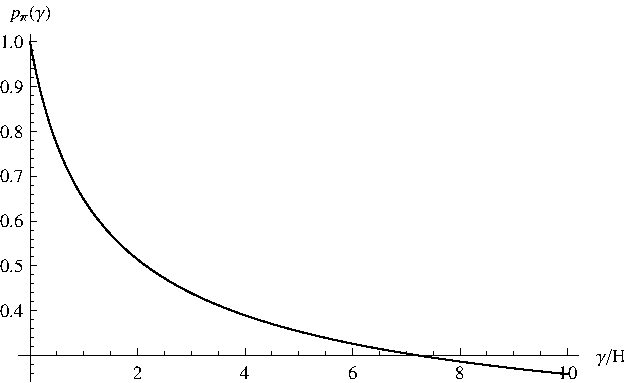
\includegraphics[width=8.5cm]{PowvsGamma}\par\smallskip
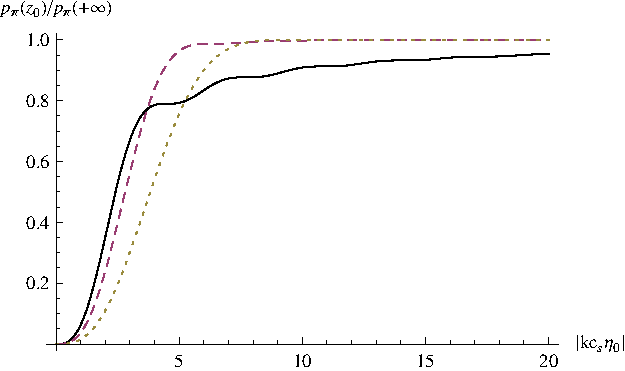
\includegraphics[width=8.5cm]{Powvsz0CG}
\caption{上：$z_0\to+\infty$における、式(\ref{pow1gamma})のパワースペクトルの$\gamma$依存性。$p_\pi(\gamma)=6N_c^2(kc_s)^3P_\pi(k)/(\pi\nu_{\calo})$と規格化した。下：$|kc_s\eta|\to0$におけるパワースペクトル$P_\pi(k)$の$z_0$依存性。$\gamma/H=0$（実線）、$\gamma/H=3$（破線）、$\gamma/H=9$（点線）を示す。}\label{casom}
\end{figure}

ADOFが（高い）温度$T$で熱平衡にあると仮定すると、FD定理から次が得られる。

\beq
\label{tempz}
k^3\langle\zeta_k\zeta_k\rangle_T \simeq  \sqrt{\pi\gamma_\star H_\star} \frac{TH_\star^2}{2c_s^\star\left({c^\star_s}^2N_c\right)}.
\eeq

これらは、数値因子を除けば式(\ref{tpnuo},\ref{tpwarm})の結果とまさに一致する。式(\ref{tempz})と類似した表式は文献\cite{berera1,berera2}で初めて導入され、温かいインフレーション模型\cite{warm}で重要な役割を果たす。

いくつか補足しておく。まず、一連の演算子を単一の演算子$\calo\pi$にまとめているため、扱う項の種類によって局所近似の見え方は大きく異なる。しかし、仮定を課した後の解析はかなり頑健であり、模型の細部には依存しない。保証する必要がある唯一の制約は2点関数のスケール不変性であり、これはインフレーション中に$\gamma,\nu_{\calo}$が比較的一定に保たれる限り保証される（詳細は後述する）。

非線形の次数に進むと、模型間の違いが役割を持ち始める。たとえば、摩擦項は演算子$\calo_\mu\delta g^{\mu0}$のみに由来するかもしれず、その場合は$\calo$と$\pi$の非線形結合を生じない。あるいは、スカラー結合$f(t)\calo$または$\calo\delta g^{00}$によって生じるかもしれず、その場合には互いにかなり異なる非線形相互作用が生じる。前述のとおり、$\calo\delta g^{00}$は最も明確な場合と考えられ、$f_{\rm NL}$の値が摩擦係数と結びつく。$f(t)\calo$では必ずしもそうならず、非Gaussian性の大きさは模型の詳細に依存する。しかし、前に論じたように、優先的な時計が1つだけ存在し、（非線形）応答$\delta\calo_R$が創発的シフト対称性を持つ場合には、$f_{\rm NL}$も同じように増大する。以下では、この解析をより精密にする。

\sectionlink{非Gaussian性}\label{nongaus}

本論文で論じた模型の非Gaussian的特徴は、観測的な特徴という観点からは、おそらく最も興味深い結果である。実際、2点関数は準de Sitter空間の対称性によって本質的に定まり、全体の振幅と傾きというわずか2つのパラメータで特徴づけられるのに対し、高次相関関数は関数としての自由度を持つ。それが観測されれば、それを生み出す物理機構について、はるかに多くの情報を読み解くことができる。

導入した広範な演算子のクラスについて非Gaussian的特徴を網羅的に調べることは、主としてその一般性ゆえに困難であり、本論文の範囲を超える。そこで、最低次の（スカラー）演算子$\calo\delta g^{00}$と$f(t)\calo$に注目する。非常に興味深いことに、対称性を課すことによって、運動方程式の線形寄与と非線形寄与の一部を関係づけられ、大きな散逸が大きな非Gaussian性と結びつくことを示す。続く各節では散逸が$\gamma\dot\pi$の形をとると仮定する。高階微分の散逸については\ref{localo2}節で調べる。

\subsectionlink{\texorpdfstring{$\calo\delta g^{00}$}{O δg⁰⁰}}\label{Nolocalo2}

ここでは、支配的な相互作用項が$\pi$の時間微分を1つ含み、$-\calo\delta g^{00}$という形のスカラー演算子によって生じる状況を解析する。この項には$\dot\pi$に線形な部分、より正確には$2\calo\dot\pi$が含まれる（以下では式(\ref{g00pi})による因子2を演算子$\calo$に吸収し、$\calo\to\calo/2$とする）。

ここでは、\ref{localapp}節で説明した局所近似について選択肢がある。すなわち、$\langle\delta\calo_S\delta\calo_S\rangle$と$G^{\calo}_{\rm ret}$に適用することも、$\langle\delta\dot\calo_S\delta\dot\calo_S\rangle$と$G^{\dot\calo}_{\rm ret}$に適用することもできる。前者の場合、通常の散逸項$\gamma\dot\pi$ではなく、ADL力に見られるような高階微分項が得られる。ここでは後者を解析し、前者は\ref{localo2}節で論じる。

$\delta\calo_S$の時間変化のスケールを$1/H$よりはるかに短いとするので、雑音への主な寄与は$\delta\dot\calo_S\gg H\delta\calo_S$から来る。すると、基本的には\ref{localapp}節と同じ手順により、線形次数での$\pi$の方程式が、式(\ref{fineom})で$\delta\calo_S$を$\delta\dot\calo_S$に置き換えたものに帰着することを示せる。パワースペクトルは、式(\ref{pow1gamma})において$\nu_{\calo}\to\nu_{\dot\calo}$と置き換えたもので与えられる。より明示的には、2次までの$\pi$の方程式は次となる。

\beq
\ddot\pi + 3H\dot\pi  - \frac{c_s^2\nabla^2}{a^2}\pi = -N^{-1}_c\left(\delta\dot{\calo} (1+\dot{\pi})+\delta\calo\ddot\pi -\frac{1}{a^2}\partial_i(\delta\calo\partial_i\pi)\right),\label{pieqnlprev}
\eeq

ここで$\delta\calo=\delta\calo_S+\delta\calo_R$である。式(\ref{g00pi})から、$\delta\calo$を擾乱する力は$F=\dot\pi+\dot\pi^2/2-(\partial_i\pi)^2/2$と分かる。ただし、\ref{localapp}節と同様に、応答部分の時間微分$\delta\dot\calo_R$に局所近似を用いると、次が得られる。

\beq
\label{ocaldot}
\delta\dot\calo_R\simeq N_c\gamma\left(\dot{\pi} +\frac{\dot{\pi}^2}{2}-\frac{\partial_i\pi\partial_i\pi}{2 a^2}\right).
\eeq

\ref{nonlineff}節ですでに述べたように、この局所近似だけでは、追加の仮定なしに非Gaussian性へのすべての寄与を計算することはできない。式(\ref{pieqnlprev})には$\delta\dot\calo$だけでなく$\delta\calo$も現れるためである。一般に、EFTの観点から精妙な相殺は予期されず、式(\ref{ratiogk})で見積もったように、非局所項の非Gaussian性への寄与は局所項の寄与と同程度と予想される。したがって以下では、$\dot\calo$のみを含む項に注目し、式(\ref{pieqnlprev})を次に簡約する。

\beq
\ddot\pi + (3H+\gamma)\dot\pi  - \frac{c_s^2\nabla^2}{a^2}\pi =\frac{\gamma}{2}\frac{\partial_i\pi\partial_i\pi}{a^2}-\frac{3\gamma}{2}\dot{\pi}^2 -N^{-1}_c\delta\dot{\calo}_S (1+\dot{\pi}).\label{pieqnl}
\eeq

まず右辺第1項$\gamma(\partial_i\pi)^2$の寄与に注目しよう。非Gaussian性を解析するため、$\pi=\pi_1+\pi_2$と分解する。添字は通常どおり、揺らぎに関する解の次数を表す。すると、

\be\label{pi1nl}\pi_1(k,\eta)=\frac{ k c_s}{N_cH^2}\int^{\eta}_{\eta_0} d\eta' g_{\gamma}(k c_s|\eta|,k c_s|\eta'|) \delta\dot{ \calo}_S,\ee

となる。ここで$g_{\gamma}(kc_s|\eta|,kc_s|\eta'|)=G_{\gamma}(kc_s|\eta|,kc_s|\eta'|)/(kc_s\eta')^2$であり、$G_{\gamma}$は式(\ref{greengamma})で定義される。また、式(\ref{pi1nl})を用いると、

\begin{eqnarray}
\pi_2(k_3,0)&=&\frac{\gamma k_3 c_s^3}{2 N_c^2H^4} \int^0_{\eta_0} d\eta' {\eta'}^2  g_{\gamma}(0,k_3c_s|\eta'|)\int\frac{d^3{\bf q}}{(2\pi)^3} |{\bf q}|  |{\bf k}_3-{\bf q}| ({\bf q}\cdot({\bf k}_3-{\bf q}))\nonumber\\
&\times&\int^{\eta'}_{\eta_0} d\eta'' g_{\gamma}(qc_s|\eta'|,qc_s|\eta''|) \int^{\eta'}_{\eta_0} d\eta''' g_{\gamma}(|{\bf k}_3-{\bf q}| c_s|\eta'|,|{\bf k}_3-{\bf q}| c_s|\eta'''|) \nonumber\\&\times&\delta\dot{\calo}_S({\bf q},\eta'')\delta\dot{\calo}_S({\bf k}_3-{\bf q},\eta''').\label{pi2nl}
\end{eqnarray}

となる（$\pi_2$の源は、摂動$\delta\dot\calo_S,\pi_1$について2次の項である）。

$\eta\to0$の極限における$\zeta\simeq-H\pi$の3点関数を計算したい。

\begin{eqnarray}\langle\zeta({\bf k}_1,0)\zeta({\bf k}_2,0)\zeta({\bf k}_3,0)\rangle&=&\langle\zeta_1({\bf k}_1,0)\zeta_1({\bf k}_2,0)\zeta_2({\bf k}_3,0)
\rangle+ \mbox{$k_i$の巡回置換の和}\nonumber\\
&\equiv&(2\pi)^3 \delta^{(3)}({\bf k}_1+{\bf k}_2+{\bf k}_3) F(k_1,k_2,k_3). \end{eqnarray}

式(\ref{twop1})、(\ref{twop2})と、雑音がGaussianであるという条件（非Gaussian雑音は後で考える）、すなわち

\begin{eqnarray}\label{os}&&\langle\delta\dot{ \calo}_S({\bf k}_2,\tilde{\eta'}) \delta\dot{\calo}_S({\bf k}_1,\tilde{\eta})  \delta\dot{\calo}_S({\bf q},\eta'')
\delta\dot{\calo}_S({\bf k}_3-{\bf q},\eta''')\rangle=(2\pi)^6\nu_{\dot{\calo}}^2\frac{\delta^{(3)}({\bf k}_1+{\bf k}_2+{\bf k}_3)}{a^4(\eta'')a^4(\eta''')}\\
&&\times \left\{\delta(\tilde{\eta'}-\eta'')\delta(\tilde{\eta}-\eta''')\delta^{(3)}({\bf k}_2+{\bf q})+
\delta(\tilde{\eta}-\eta'')\delta(\tilde{\eta'}-\eta''')\delta^{(3)}({\bf k}_1+{\bf q})\right\}\,\,\,(\mbox{ただし} \,\,\,k_3\neq 0)\nn,
\end{eqnarray}

を用い、任意の運動量スケール$k$に対して$x_i=k_i/k$と定義すると、$\eta_0\to-\infty$で次を得る。

\begin{eqnarray}\label{fdeltagooshape}
&&F(x_1,x_2,x_3)= k^6 F(k_1,k_2,k_3)=-\frac{\gamma H^3\nu_{\dot{\calo}}^2}{2N_c^4c_s^8}x_1^2x_2^2x_3(x_3^2-x_2^2-x_1^2)\int_{0}^{+\infty} dy y^2  g_{\gamma}(0,x_3 y)\\
&&\times\int_{y}^{+\infty} dz\,{z}^4 \,g_{\gamma}(x_2 y,x_2 z)  g_{\gamma}(0,x_2 z)\int_{y}^{+\infty} dw\,{w}^4 \,g_{\gamma}(x_1 y,x_1 w) g_{\gamma}(0,x_1 w)+\mbox{$x_i$の巡回置換の和}\nn
\end{eqnarray}

ここでは$y'=-kc_s\eta'$、$z=-kc_s\eta''$、$w=-kc_s\eta''$という変数変換を行った。

対応するパラメータ$f_{\rm NL}^{\rm eq}$（正三角形配置に対して定義する）は、次で与えられる。

\be F(1,1,1)=\frac{18}{5}f_{\rm NL}^{\rm eq}\Delta^2_{\zeta},\ee

ここで$\Delta_{\zeta}=k^3P_{\zeta}$である。Green関数を用いて表すと、

\begin{eqnarray}
f_{\rm NL}^{\rm eq}&=&\frac{5}{12}\left(\frac{\gamma}{Hc_s^2}\frac{2^{-8\gamma/H}\pi^2 {\Gamma\left(\frac{2\gamma}{H}+4\right)}^2}{\lp\frac{\gamma}{H}+1\rp^6{\Gamma\lp\frac{\gamma+H}{2 H}\rp}^8}\right)
 \int_{0}^{+\infty} dy {y}^2 g_{\gamma}(0, y)\int_{y}^{+\infty} dz z^4  g_{\gamma}( y,z)g_{\gamma}(0, z) \nonumber\\
&\times&\int_{y}^{+\infty} dw w^4  g_{\gamma}( y,w)g_{\gamma}(0, w),\label{fnlgoonoloc}
\end{eqnarray}

となる。ここでは式(\ref{pow1gamma})のパワースペクトルを、$\nu_{\calo}\to\nu_{\dot\calo}$として用いた。数値積分を行うと、

\beq
\label{fnlNL}
f_{\rm NL}^{\rm eq}\simeq-\frac{\gamma}{4H c_s^2},\eeq

が強散逸領域$\gamma\gg H$で得られる。$c_s\simeq1$であっても、これは大きくなりうる。文献\cite{Senatore:2009gt}の解析を用いると、桁の程度の上限も示すことができる。

\beq
\label{boundfnl}
\frac{\gamma}{H c_s^2} \lesssim 500.
\eeq

図\ref{shapegoonoloc}では、2つの$\gamma$の値（$\gamma=4H$および$40H$）について形状を描いた。正三角形配置にピークがあり、$x_2\simeq x_3\simeq1/2$の付近にも別のピークがあることに注意されたい。後者はバイスペクトルの主要な特徴の1つであり、揺らぎが雑音に支配されていることに由来する。

$\gamma\gg H$であってもその値が中程度の場合、形状は文献\cite{Senatore:2009gt}で述べられた直交型に似ている。この直交型は、現在のWMAP 7年データ\cite{Komatsu:2010fb}では$2\sigma$の水準にある。

\begin{figure}[htp]
\centering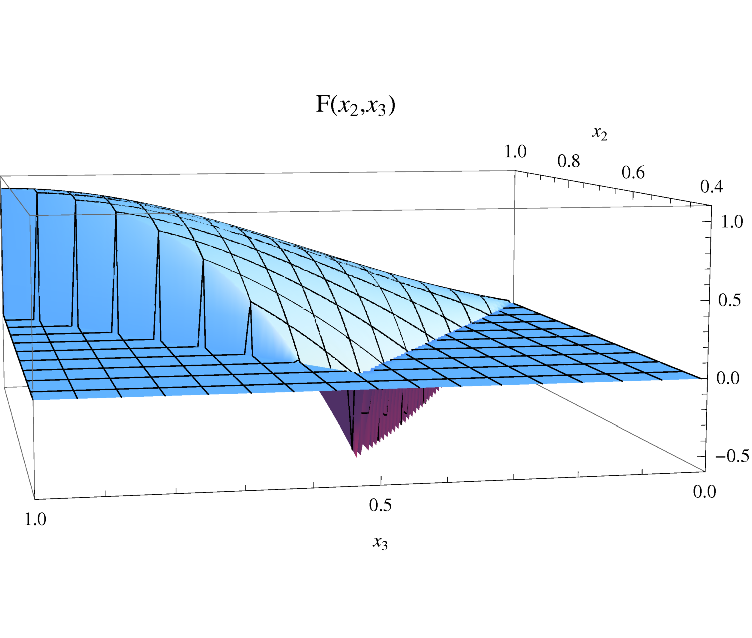
\includegraphics[width=8.5cm]{deltag00Noloc4}\par\smallskip
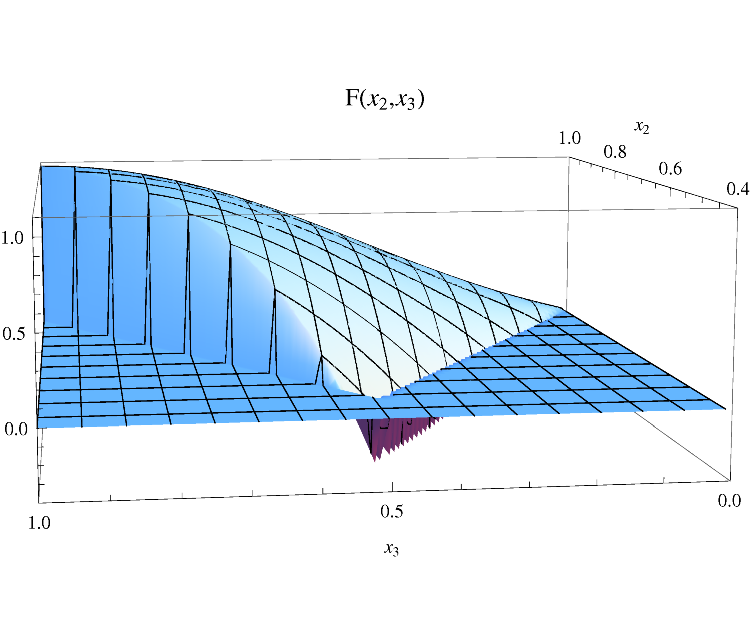
\includegraphics[width=8.5cm]{deltag00Noloc40}
\caption{式(\ref{fdeltagooshape})で与えられる形状$F(x_2,x_3)=x_2^2x_3^2\frac{F(1,x_2,x_3)}{F(1,1,1)}$。$\gamma=4H$（上）および$\gamma=40H$（下）の場合を示す。等価な配置の重複表示を避けるため、$1-x_2\leq x_3\leq x_2$の領域外では関数を0としている。}\label{shapegoonoloc}
\end{figure}

同様に、式(\ref{pieqnl})の右辺第2の源の項に対して、次を得る。

\begin{eqnarray}
f_{\rm NL}^{\rm eq}&=&-\frac{5}{2}\frac{\gamma}{H}\left(\frac{2^{-8\gamma/H}\pi^2 {\Gamma\left(\frac{2\gamma}{H}+4\right)}^2}{\lp\frac{\gamma}{H}+1\rp^6{\Gamma\lp\frac{\gamma+H}{2 H}\rp}^8}\right)
 \int_{0}^{+\infty} dy  g_{\gamma}(0, y)\int_{y}^{+\infty} dz z^4  y\frac{d g_{\gamma}}{dy}( y,z)g_{\gamma}(0, z) \nonumber\\
&\times&\int_{y}^{+\infty} dw w^4  y\frac{dg_{\gamma}}{dy}(y,w)g_{\gamma}(0, w).\label{fnlgoonolocdot1}
\end{eqnarray}

見かけによらず、この項の$f_{\rm NL}^{\rm eq}$への寄与は$\gamma$とともに増大せず、1の程度の副次的な効果となる。これはGreen関数の性質から従い、特に時間微分が$\sqrt{\gamma H}$ではなく$H$のべきでスケールすることによる。凍結時のGreen関数がそのような時間依存性を持つためである。これは、\ref{noise}節の平坦時空での結果（「$\tau_{\rm eq}$」$\sim1/H$）からまさに予想されることである。これらのGreen関数に関する詳細のまとめは付録\ref{greenf}を参照されたい。

式(\ref{pieqnl})の最後の項については、次が得られる。

\begin{eqnarray}\label{fnlOdotpi}
f_{\rm NL}^{\rm eq}&=&\frac{5}{3}\left(\frac{2^{-8\gamma/H}\pi^2 {\Gamma\left(\frac{2\gamma}{H}+4\right)}^2}{\lp\frac{\gamma}{H}+1\rp^6{\Gamma\lp\frac{\gamma+H}{2 H}\rp}^8}\right)
 \int_{0}^{+\infty} dy  y^4\, (g_{\gamma}(0, y))^2\int_{y}^{+\infty} dz z^4  y\frac{d g_{\gamma}}{dy}(y,z)g_{\gamma}(0, z),\label{fnlgoonolocdot2}
\end{eqnarray}

これも1の程度の寄与であり、$\gamma$とともに増大しない。この項に対応する形状を、$\gamma=10H$の場合について図\ref{ngg10}に示す。

予想どおり、これらの形状はすべてスクイーズド極限に近づくと抑制される。寄与が$\pi$の時間微分を含み、また$\delta{\cal O}$が局所的だからである。この極限とは、運動量の1つ、たとえば$k_1\equiv k_L$（長波長モード）が、他の2つ（短波長モード）よりはるかに小さい場合、すなわち$k_L\ll k_S$（$k_S=|{\bf k}_2-{\bf k}_3|/2$）である。ただし、興味深い問題が残る。それは、この抑制が局所型の形状と比べて$k_L$の1乗、あるいはそれ以上のべきを伴うかどうかである。この特定のスケーリングにより、スケール依存バイアスの測定において単一場模型の特徴を識別できる可能性があるためである\cite{creminelli11}。この点には次節で戻る（図\ref{ngg10}から、形状そのものがスクイーズド極限$k_L/k_S\to0$で0に近づくことを指摘しておく。したがって$F(x_1,x_2,x_3)$は$1/x_L^2\equiv(k_S/k_L)^2$のようにはスケールせず、それより弱いべきで振る舞う）。

\begin{figure}[htp]
\centering
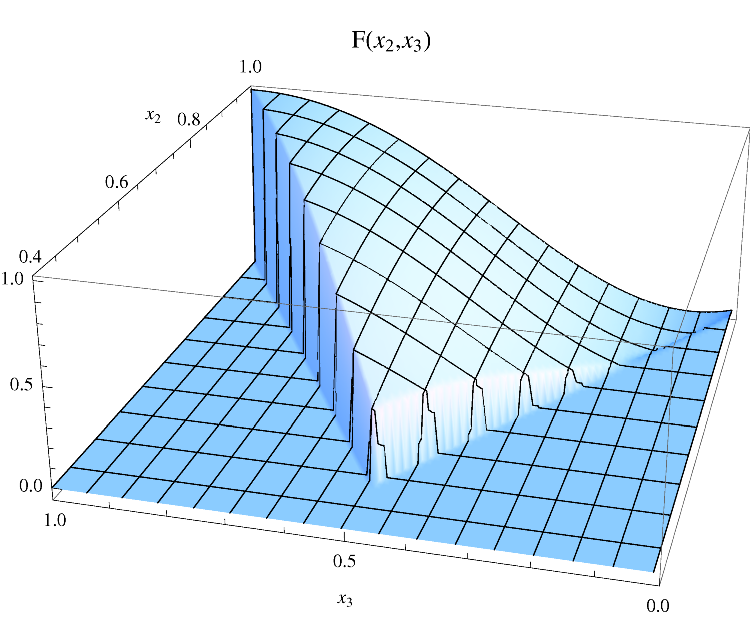
\includegraphics[width=8.5cm]{NGGamaOdotpigamma10}
\caption{式(\ref{pieqnl})の最後の項に対応する、$\gamma=10H$の場合の形状$F(x_2,x_3)=x_2^2x_3^2\frac{F(1,x_2,x_3)}{F(1,1,1)}$。}\label{ngg10}
\end{figure}

\subsectionlink{\texorpdfstring{$f(t)\calo$ I：線形応答}{f(t)O I：線形応答}}\label{ftcalo}

今度は、式(\ref{inter1n})にあるような$f(t)\calo$の形の相互作用による寄与を考えよう。可能性を線形応答と非線形応答の2つに分け、後者は次節で扱う。

線形応答理論で非線形効果を計算するため、ADOFに作用する力を$\pi$の2次まで用いる。これは$F=\dot f\pi+\ddot f\pi^2/2+\ldots$で与えられ、省略記号は$f(t)$の高階時間微分に比例する、$\pi$のより高いべきの項を表す。\ref{appsh}節で述べたように、一般にはスローロール近似でこれらの項を無視する。したがって以下では、$\dot f$を本質的に一定として扱う。

$G_{\rm ret}^{\calo}$の局所近似のもとで、応答部分$\delta\calo_R$は次のように書ける。

\be
\label{ddff}
\delta\calo_R\simeq \frac{\gamma N_c}{\dot{f}}\left(\dot{\pi}+\frac{\ddot{f}}{\dot{f}}\dot{\pi}\pi\right),
\ee

ここでは、スローロールパラメータのより高いべきで抑制される項を除いた（微分を含まない項を無視するため、創発的シフト対称性の存在を仮定していることを思い出されたい）。したがって、$\pi$の2次までの方程式は次となる。

\be\label{pia}
\ddot{\pi}+(3H+\gamma)\dot{\pi}+\frac{k^2c_s^2}{a^2}\pi+2\gamma\frac{\ddot{f}}{\dot{f}}[\pi\dot{\pi}]_k=-N_c^{-1}\left(\dot f\delta \calo_S+\ddot{f}[\pi\delta \calo_S]_k\right),
\ee

ここで雑音部分$\delta\calo_S$は式(\ref{twop1},\ref{twop2})を満たす。この方程式を式(\ref{fineom})と比較すると、パワースペクトルは全体の因子$\dot f^2$を除いて式(\ref{pow1gamma})と同じである。すなわち、$\nu_{\calo}\to\nu_{f\calo}=\dot f^2\nu_{\calo}$とすればよい。したがって、パワースペクトルのスケール不変性を保証するには、$\dot\nu_{f\calo}/(\nu_{f\calo}H)\simeq O(\epsilon)$が必要である（これについては後で詳しく述べる）。

\ref{appsh}節で強調したように、上の非線形項による$f_{\rm NL}$への寄与は$\ddot f/(\dot fH)\simeq O(\epsilon)$で抑制される。この次数では、重力との混合などの他の効果をもはや無視できないことに注意されたい。さらに、次節で非Gaussian性が非線形応答によって支配されることを示す。それでもここに式(\ref{pia})の項の計算を含めるのは、2つの理由による。まず、非線形項は$\gamma$に比例していても、最終的な答えではその因子が消えることを明示するためである。より重要なのは、$\dot f$が定数でない場合、スクイーズド極限で無視できないかもしれない寄与を与えるように見えるためである。

まず式(\ref{pia})の最後の源の項$\ddot f\pi\delta\calo_S$を解析しよう。この項は$\pi$の微分を十分には含まないため、$F(x_2,x_3)=x_2^2x_3^2\frac{F(1,x_2,x_3)}{F(1,1,1)}$で与えられる形状の寄与がスクイーズド極限で最大となることは容易に分かる。その極限では、パラメータ$f_{\rm NL}$は次で与えられる。

\begin{equation}\label{squ}
f_{\rm NL}^{\rm sq} =\lim_{x_3\to 0,\,\ x_2\to 1}\frac{5}{6} \frac{F(1,x_2,x_3)}{(P_{\zeta}(1)P_{\zeta}(x_2)+P_{\zeta}(1)P_{\zeta}(x_3)+P_{\zeta}(x_2)P_{\zeta}(x_3))}.
\end{equation}

前節までと同様の手順に従うと、次を得る。

\beq f_{\rm NL}^{\rm sq}\simeq-\frac{5 }{6}\frac{\ddot{f}}{H\dot{f}} \label{fnlddf},\eeq

これは$\gamma$の値によらない。式(\ref{estfto})の先の見積もりと一致する。同様に、式(\ref{pia})の左辺最後の項の寄与も計算できる。この項は$\gamma$に比例するが、パラメータ$f_{\rm NL}$は上の値に比べて顕著には増大しない。これは\ref{appsh}節の発見的議論から従うが、Green関数の性質から直接見ることもできる。付録\ref{greenf}を参照されたい。近似的シフト対称性が$\ddot f/(H\dot f)\simeq O(\epsilon)$を要請するため、前述のとおり式(\ref{fnlddf})の$f_{\rm NL}^{\rm sq}$は非常に小さくなる。

それでも、パワースペクトルに現れる組み合わせ$\nu_{f\calo}=\dot f^2\nu_{\calo}$を一定に保つ一方で、$\dot f,\nu_{\calo}$は近似的に一定でないと仮定した場合、式(\ref{fnlddf})の結果が気になるかもしれない。しかし上の計算は不完全である。非線形の次数では、$\pi$が雑音の確率密度汎関数にも影響することによる寄与があるためである（これらは$\dot\nu_{\calo}\ll H\nu_{\calo}$の極限で抑制される）。すべての寄与を考慮すれば、地平線の外に時計以外のいかなる摂動も含めていないという事実と整合するために、最終的には$f_{\rm NL}^{\rm sq}$は$(n_s-1)$に比例するはずである\cite{consist,Cheung:2007sv}。

スクイーズド極限の性質をよりよく理解するために、本研究でよく現れる$\delta\calo\dot\pi$型と$\delta\calo\pi$型の非線形性の寄与を比較しよう。両者で$\calo$演算子を同じものに固定すると、重要な違いは、後者の形状が$g_\gamma(x_Ly,z)$を含むのに対し、前者は$y\partial_yg_\gamma(x_Ly,z)$を含むことであると容易に分かる（$z,y$は積分変数）。次を用いると、

\beq
\frac{y\partial_{y}g_{\gamma}(x_L y, z)}{  g_{\gamma}(x_L y, z)}\sim \frac{x_L^2y^2}{(1+\gamma/H)},
\eeq

これは$yx_L\ll1$で成り立ち、積分が$\sqrt{\gamma/H}$付近の$y,z$の値に支配されること（付録\ref{greenf}参照）も考慮して、$x_L^2\ll H/\gamma$の領域では、$\delta\calo\dot\pi$のスクイーズド極限は$\delta\calo\pi$の寄与に比べて$x_L^2=(k_L/k_S)^2$の因子で抑制されると結論できる。これは文献\cite{creminelli11}の結果と一致する。スクイーズド極限と整合性条件については、別の機会により詳しく議論する。

次に、非Gaussian性への最大の寄与を与えることになる$f(t)\calo$結合の非線形応答を調べる。

\subsectionlink{\texorpdfstring{$f(t)\calo$ II：非線形応答}{f(t)O II：非線形応答}}\label{nonlrep}

これまでは、応答$\delta\calo_R$を$\pi$の線形次数で考えてきた。そのために必要なのは2点関数$G_{\rm ret}^{\calo}$のみである（式(\ref{gnoa1})参照）。しかし、$\delta\calo$の高次の$n$点関数へ進むことによっても非線形性を誘起できる。たとえば、その3点関数

\beq
C^{\calo}_{\rm ret} (x,y,z) \equiv \langle [\delta\calo(z),[\delta\calo(y),\delta\calo(x)]]\rangle \theta(t_y-t_z)\theta(t_x-t_y),
\eeq

を含め、力は最低次の$F(\pi)=\dot f\pi$のままにする（以下では$\dot f$を定数として扱う）。すると、

\beq
\label{calo12}
\dot f \delta\calo_R(x) = -\dot f^2 \int G^\calo_{\rm ret}\pi(y) dy + \dot f^3 \int dydz~C^{\calo}_{\rm ret}(x,y,z)\pi(y)\pi(z) + \ldots
\eeq

となる。省略記号は高次の補正を表す。

先験的には、両者が空間と時間について局所的であると仮定しても、$G_{\rm ret}^{\calo}$と$C_{\rm ret}^{\calo}$の間に関係は期待されない。しかし、以下で論じるように、ADOFの応答が単一の（優先される）時計によって支配される場合には、両者の関係が得られる。

本論文を通して強調したように、演算子$f(t)\calo$から散逸項を得るためには、局所的なGreen関数を仮定すると、次が必要である。

\beq
\dot f  \delta^{(1)}\calo_R = N_c \gamma \dot\pi.
\eeq

この式は示唆的な形に次のように書き換えられる。

\beq
\label{onecalR}
\dot f  \delta^{(1)}\calo_R = N_c \gamma~\delta^{(1)}\left\{n^\mu\partial_\mu(t+\pi)\right\},
\eeq

ここで（$O(\pi^2)$を除いて$n^0=1$であることに注意されたい）、

\beq
\label{nmu2} n^{\mu}=\frac{-g^{\mu\nu}\partial_{\nu}{\tilde t}}{\sqrt{-g^{\nu\rho}\partial_{\nu}{\tilde t}\partial_{\rho}{\tilde t}}},
~~\tilde t = t+\pi, \eeq

とする。これにより、式(\ref{onecalR})は$\calo$がスカラー演算子であるという対称性を明示する。すると、応答を$\pi$の全次数に外挿でき、次が得られる。\footnote{原理的には、これは$F_\calo\left(\sqrt{-g^{\nu\rho}\partial_\nu\tilde t\partial_\rho\tilde t}\right)$へ一般化できる。簡単のため、$F_\calo(x)=x$に限定する。}

\beq
\label{gretto2p}
\dot f  \delta^{(n)}\calo_R = N_c \gamma~\delta^{(n)}\left\{n^\mu\partial_\mu(t+\pi)\right\} = N_c\gamma~\delta^{(n)}\left(\sqrt{-g^{\nu\rho}\partial_{\nu}{\tilde t}\partial_{\rho}{\tilde t}}\right).
\eeq

この式が、運動方程式における線形項と非線形項の関係を意味することは容易に示せる。たとえばユニタリーゲージ、すなわち$\tilde t=t$では、

\beq
\label{dpcalfn}
\dot f  \delta^{(n)}\calo_R = N_c \gamma~\delta^{(n)}\sqrt{-g^{00}},
\eeq

となり、$g^{00}(\pi)=-1-2\dot\pi-\dot\pi^2+(\partial_i\pi)^2$を用いて$\pi$の相互作用を読み取れる。したがって、

\bea
-\dot f \delta^{(1)}\calo_R &=& -N_c \gamma \dot\pi,\\
-\dot f \delta^{(2)}\calo_R &=& \frac{1}{2} N_c \gamma (\partial_i\pi)^2 
\label{dpcalo2}.
\eea

となる。こうして、厳密なシフト対称性の場合に得られたものと似た非線形項が得られる（式(\ref{pieqnl})の右辺第1項を参照し、式(\ref{ocaldot})とも比較されたい）。\footnote{式(\ref{dpcalfn})の型の非線形応答では$\dot\pi^2$項が得られなかったことに注意されたい。しかし、一般的な関数$F_\calo(\sqrt{-g^{00}})$を許せば、この項も生じうる。}非Gaussian性の解析は\ref{Nolocalo2}節と同様に進み（\ref{shsym}節も参照）、

\beq
f_{\rm NL} \simeq -\frac{\gamma}{c_s^2 H},
\eeq

となる。これは\ref{nlrep}節で予想したとおりである。形状も図\ref{shapegoonoloc}に似たものとなる。

前の議論は、従来のスカラー場インフレーション模型に限定すると、より分かりやすいかもしれない。重要な点は、摂動への応答が微分同相不変性と整合しなければならないことである。そのため散逸を誘起するには$\dot\phi$の因子が必要であり、それがさらに、\ref{nlrep}節で概略を述べたように、$\gamma\gg H$の場合に大きな非Gaussian性をもたらす。

論理は次のとおりである。$\calo$をスカラー演算子として、次の形の相互作用Hamiltonianを考えよう。

\beq
H_{\rm int} = \phi\; \calo \label{hint}.
\eeq

インフラトンの運動方程式は、したがって次となる。

\beq
\label{eomphi}
D_\phi \phi = \calo,
\eeq

ここで$D_\phi\phi=0$は$\calo$が存在しない場合の運動方程式を表す。もちろん、$\calo$の背後には独自の$\calL_\calo$を持つ力学系がある。しかし、EFTの考え方に従い、式(\ref{hint})の結合以外は何も仮定しない。まず背景$\bphi(t)$を求めることから始める。局所的な応答を仮定すると、

\beq
\label{gcalo}
\langle \bphi|\calo |\bphi\rangle = F_\calo(\bphi, \dot{\bphi}),
\eeq

となる。括弧は、$\bphi$が与える背景で応答を計算していることを強調する。式(\ref{eomphi})に代入すると、次を得る。

\beq
\label{dphibpi}
D_\phi \bphi = F_\calo(\bphi, \dot{\bphi}).
\eeq

本論文で調べる型の、速度に依存する散逸を得るため、次を課す。

\beq
\label{fphip}
 F_\calo(\bphi, \dot{\bphi})\simeq |\dot\bphi|.
\eeq

この振る舞いの具体例を、より複雑な応答関数を用いてではあるが、\ref{matching}節で論じる。次の段階は$\bphi\to\bphi+\delta\phi$という摂動を加えることである。議論の要点は、式(\ref{gcalo})を何が置き換えるかにある。この問題に取り組む方法はいくつかあるが、おそらく最も簡単なのは次の方法である。$\calo$は構成上スカラー演算子なので、式(\ref{gcalo})を共変化しなければならない（Lorentz不変性は、優先される基準系の存在、すなわち式(\ref{nmu2})で$\tilde t$を$\phi$に置き換えた$n^\mu$によってのみ破られる）。したがって、先の議論のとおり、式(\ref{gcalo})を次のように書き換えるべきである。

\beq
\label{gcalo2}
\langle \phi|\calo |\phi\rangle = F_\calo\left(\phi, n^\mu \partial_\mu \phi = -g^{\mu\nu}\partial_\nu\phi\partial_\mu\phi/\sqrt{-g^{\mu\nu}\partial_\nu\phi\partial_\mu\phi}\right),
\eeq

ここでは関数$F_\calo$が本質的には変化しないと仮定した。これは$\delta\phi$が滑らかな長波長摂動であれば妥当な局所近似である。\footnote{言い換えると、明確に定義された微分展開を持つために、等時刻面の外部曲率の変化スケール（$K^{ij}\simeq\nabla^i_{(3)}n^j$に注意）が、$\phi$と$\calo$の相互作用の局所近似を支配する典型的長さスケール$M_\calo^{-1}$よりはるかに大きい必要がある。たとえば地平線通過時の摂動$\delta\phi_{k_\star}$をとり、$g$を結合定数として$M_\calo^2\simeq g|\dot\bphi|$とすれば、$k_\star^2\ll M_\calo^2$、あるいは$\gamma<g|\dot\bphi|/H$が必要である（完全に一般的には、抑制されていても$\delta K_{\mu\nu}$による補正も原理的には含めるべきである）。詳細は\ref{localtrap}節を参照されたい。}

再びユニタリーゲージに移り、$\phi=\bphi$、すなわち$\delta\phi=0$となる座標を選ぶ。これは次を意味する。

\beq
\label{gcalo3}
\langle \phi| \calo |\phi \rangle = F_\calo\left(\bphi,\dot\bphi\sqrt{-g^{00}}\right).
\eeq

次に、式(\ref{dphibpi})とSt\"uckelbergの方法を用いて摂動$\delta\phi$（ここでの$\pi$）を導入する。左辺には通常の項が得られ、右辺には式(\ref{fphip})の要請を用いると、

\beq
D_\phi \delta\phi  \simeq \delta \left(|\dot\bphi| \sqrt{-g^{00}(\pi)}\right),
\eeq

となる。これは式(\ref{dpcalfn})から得られた結果に似ており、$\pi=\delta\phi/\dot\bphi$である。そして前述のとおり、散逸項$\gamma\dot\pi$に加えて$\gamma(\partial_i\pi)^2$も得られ、\ref{Nolocalo2}節で示したように、これによって非Gaussian性が増大する。

前の議論には、強調しておくべき微妙な点がある。厳密には、散逸の存在が要求するのは$\pi$への線形結合のみである。我々の議論で式(\ref{gretto2p})の$n^\mu\partial_\mu\pi$から得られた非線形項は、$n^\mu$が、インフレーションの終了を制御する物理的時計の一様なスライスに直交する時間的ベクトルであることと本質的に結びついていた。しかし一般には、ADOFに時間的ベクトル演算子が含まれることもあり、これらをまとめて$u_\calo^\mu$と書くと、背景で非ゼロの期待値を持ちうる。したがって、式(\ref{gretto2p})には$n^\mu\partial_\mu\pi$に代わって$u_\calo^\nu\partial_\nu\pi$が現れるかもしれない。\footnote{これは、$\calo$の応答が$u_\calo^\mu$によって制御される場合に起こりうる。}その場合、線形項$\gamma\dot\pi$（今度は$\langle u_\calo^\mu\rangle=(1,0,0,0)$から導かれる）と、その非線形の対応物との関係は保証されない。この状況では、大きな散逸が必ずしも強い非Gaussian性をもたらすとは限らない。

\ref{newdof}節で導入したGoldstoneボソン$\tilde\pi$を直接用いることを選んでいれば、非ゼロの期待値をとるベクトル型演算子は存在しなかったはずである。この場合、背景の期待値を持つ唯一のベクトルは、規格化を除けば$n^\mu\sim g^{\mu\nu}\partial_\nu(t+\tilde\pi)$となり、式(\ref{dpcalo2})の型の項を誘起するように見える。しかし2つの記述は等価である。実際、模式的に$\tilde\pi\sim\pi+\delta O$であることに注意すると、この場合であっても、$\tilde\pi$とベクトル演算子の揺らぎ$\delta u_\mu^\calo$の相互作用により、非線形次数で式(\ref{dpcalo2})の項が生成されなくなる可能性を一般には排除できない。したがって、散逸と非Gaussian性との関係を保証するために、そのような相殺がないことを要請する。

この条件を実装する簡単な方法はない。ただし実際には、$\delta\calo$が、その揺らぎによってインフレーションの終了を制御する場$\pi$に主として感度を持つことを要請することに相当する。本論文では、この条件を「優先的な時計を持つ」と表現してきた。

したがって、そのような時計の存在は、強散逸領域において必然的に大きな非Gaussian性を伴うと結論できる。それは\ref{Nolocalo2}節で明示した$\calo g^{00}$に由来する場合も、今説明した$f(t)\calo$の非線形応答を通じて生じる場合もある。この仮定を緩めることについては今後の研究で扱う。

\subsectionlink{非Gaussian雑音}\label{ngaussnoise}

非Gaussian性の最後の源として、雑音揺らぎに内在する非Gaussian性の効果を考える必要がある。式(\ref{ngnoise})と同様に、局所的な非Gaussian雑音$\delta\calo_S$を考えよう。すなわち、

\beq
\langle\delta\calo_S(t_1, {\bf k}_1)\delta\calo_S(t_2, {\bf k}_2)\delta\calo_S(t_3, {\bf k}_3)\rangle\simeq (2\pi)^3\delta^{(3)}({ \bf k}_1+ {\bf k}_2+ {\bf k}_3)\nu_{{\calo}^3}\frac{\delta(t_1-t_2)}{a^{3}(t_1)}\frac{\delta(t_2-t_3)}{a^3(t_2)}.
\eeq

である。次を用いると、

\beq \pi(t, {\bf k})=\frac{\dot{f} k c_s}{N_c H^2}\int^{\eta}_{\eta_0} d\eta' g_{\gamma}(kc_s |\eta|, k c_s|\eta'|)\delta\calo_S(\eta',{\bf k})
\eeq

$\eta\to0$かつ$\eta_0\to-\infty$に対して、次を得る。

\beq\label{NGNoise}
F(x_1,x_2,x_3)=-\frac{\dot{f}^3 H^5\nu_{{\calo}^3}}{N_c^3c_s^6}x_1x_2x_3\int_0^{+\infty} dz z^8 g_{\gamma}(0,x_1 z)g_{\gamma}(0,x_2 z)g_{\gamma}(0,x_3 z).\eeq

\begin{figure}[h!]
\centering
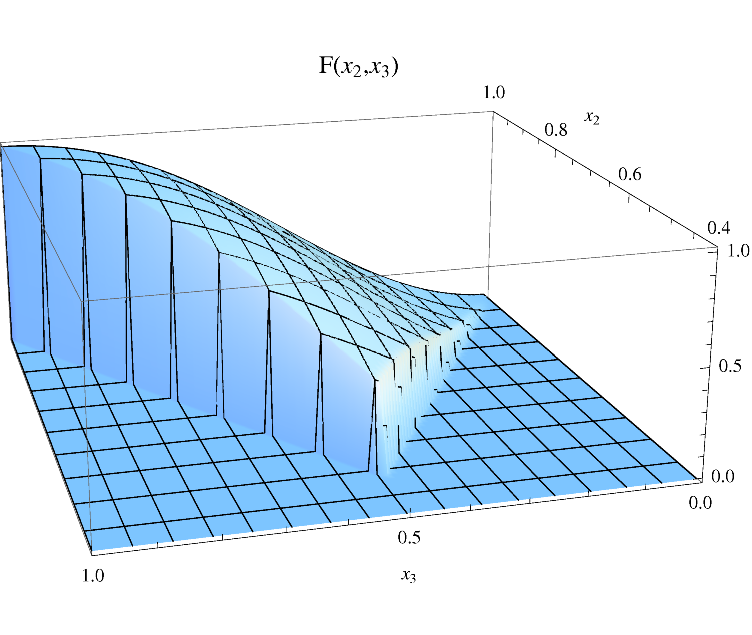
\includegraphics[width=8.5cm]{NGCG10Noise}
\caption{式(\ref{NGNoise})から得られる、$\gamma\simeq10H$の場合の形状$F(x_2,x_3)=x_2^2x_3^2\frac{F(1,x_2,x_3)}{F(1,1,1)}$。等価な配置の重複表示を避けるため、$1-x_2\leq x_3\leq x_2$の領域外では関数を0としている。}\label{nonGausNoise}
\end{figure}

形状を図\ref{nonGausNoise}に示す。予想どおり正三角形配置にピークがあり、

\beq
f_{\rm NL}^{\rm eq}\simeq \frac{\gamma N_c\nu_{{\calo}^3} }{\dot{f} \nu_{\calo}^2},
\eeq

となる。これは式(\ref{fnlnoise})で予想したとおりである。

\subsectionlink{高階微分の散逸}\label{localo2}

今度は\ref{Nolocalo2}節と同じく、支配的な相互作用$\delta g^{00}\calo$が$\pi$の微分を1つ含む状況を考えよう。ただし、前とは異なり、ここでは$\calo$の2点関数に局所近似（あるいは${\rm Im}G_{\rm ret}^{\calo}\sim\omega$）を仮定する。その結果、次が得られる。

\beq\label{eq:help}\delta\calo_R\simeq-\frac{N_c}{a^3\Gamma_\calo}\partial_t(a^3\dot{\pi}),\ee

ここで$\Gamma_\calo$は質量の次元を持ち、模型の具体的な詳細に依存する。相互作用項が$\pi\delta\dot\calo$の形であることから、運動方程式は次となる。\footnote{$H/\Gamma_\calo$の程度の音速の補正も生じるが、ここでは無視する。}

\beq \ddot{\pi}+\frac{c_s^2k^2}{a^2}\pi+3H\dot\pi- \frac{1}{\Gamma_\calo a^3}\partial_t^2(a^3\dot\pi)=-\frac{\partial_t(a^3\delta\calo_S)}{a^3N_c},\eeq

この方程式はADL力を思わせるものになっている。高階微分項の存在によって、$\omega\simeq H\ll\Gamma_\calo$に制限し、高階微分項を小さな摂動として扱わなければならない。この場合、凍結は$\omega\sim H$で起こり、主要な効果は、ここでは真空解に支配される2点関数ではなく、3点関数に現れる。これは、運動方程式の非線形項を線形項と比較することで見積もれる。2次の方程式は次のように書ける。

\be\ddot{\pi}_2+\frac{{c}_s^2k^2}{a^2}\pi_2+H\lp3+\frac{ k^2c_s^2 \delta}{a^2H^2}\rp\dot{\pi}_2=J_k,\ee

ここで$J_k$は2次の源を含む。$\pi$と$\delta\calo$の結合から、次が得られる。

\be \label{source}J_k=-\frac{1}{N_c}\left\{\frac{\partial_t(a^3{\delta}_2\calo)}{a^3}+\frac{\partial_t(a^3\dot{\pi}_1{\delta}_1\calo)}{a^3}-\frac{\partial_i({\delta}_1\calo\partial_i\pi)}{a^2}\right\},\ee

ここで$\delta\calo=\delta\calo_S+\delta\calo_R$であり、添字は寄与を$\pi$の何次まで計算するかを表す。見積もりのため、音速が小さい模型で支配的となる最後の項を考える。式(\ref{eq:help})を用いると、非Gaussian性の大きさは次で与えられる。

\be
f_{\rm NL}\zeta\sim\left.\frac{\frac{1}{N_c}\partial_i({\delta}_1\calo\partial_i\pi)}{\ddot\pi}\right|_{\omega\sim H}\sim\frac{H^4 \pi^2}{c_s^2 \Gamma_\calo}\cdot \frac{1}{ H^2\pi}\sim\frac{H}{\Gamma_\calo}\cdot\frac{1}{c_s^2}\zeta\ll \frac{1}{c_s^2}\zeta,
\ee

したがって、これは高々副次的な信号にしかなりえない。

\sectionlink{インフレーション中の散逸効果のマッチング}\label{matching}

EFTの立場では$G_{\rm ret}^{\calo}$と雑音核に対する条件を与えられたものとして扱えるが、それでも、これらの条件がある程度の近似で確かに成立する状況を特定できることが望ましい。たとえば、式(\ref{drude})のDrude模型のように、記憶効果が十分速く減衰する場合には、この記述が有効であると予想される。これは、短い相互作用時間の後に$\pi$場への逆反応が無視できるような$\calo$の力学であれば成り立つ。本節では、文献\cite{trapped}のトラップ型インフレーション模型の考え方に沿った具体的実現を調べ、温かいインフレーションの枠組み\cite{berera1,berera2,warm}についても簡単に論じる。$\calo\dot\pi$結合によって$\gamma\dot\pi$の散逸を生じる模型のクラスについては、付録\ref{mag00}を参照されたい。

\subsectionlink{\texorpdfstring{局所的なトラップ型インフレーション：$f(t)\calo\to\sum_i(\phi-\phi_i)^2\chi_i^2+\calL(\chi_i)$}{局所的なトラップ型インフレーション：f(t)O → Σᵢ(φ−φᵢ)²χᵢ² + L(χᵢ)}}\label{localtrap}

時間に関する局所近似を適用できる例を求めたい。トラップ型インフレーションでは、粒子が生成されることと、その質量が時間とともに増大することの両方によって、インフラトンのエネルギーがADOFに移される。元の模型では、宇宙膨張によって粒子が十分に希釈されるまで、これが重要である。そのための特徴的時間スケールは$H^{-1}$であり、これまで用いてきた局所的応答関数を使うことはできない。しかし、生成粒子がさらに別の自由度へ、Hubbleよりはるかに速い崩壊率で崩壊すれば、この特徴的時間スケールを大幅に短くできる。この点を念頭に置いて、トラップ型インフレーションの作用を考えよう。

\beq \label{seftrap} S_{\rm trap}=\int d^4x\sqrt{-g} \left\{\sum_i\left[-\frac{1}{2}\partial_{\mu}\chi_i\partial^{\mu}\chi_i-\frac{ g^2(\phi-\phi_i)^2}{2}\chi_i^2\right]-\frac{1}{2}\partial_{\mu}\phi\partial^{\mu}\phi-V(\phi)\right\},\eeq

ここで$\phi$はインフラトン、$V(\phi)$はそのポテンシャルである。さらに、$\chi_i$と追加の自由度$\varphi$との結合を特徴づける相互作用項$S_{\rm int}(\chi_i,\varphi)$を加える。この結合による$\chi_i$の崩壊率は$\Gamma_{\chi_i}\gg H$を満たすものとする。課す必要のある唯一の条件は、$S_{\rm int}$が$S_{\rm trap}$から得られる最低次の描像を変えないことである。特に、$\phi\simeq\phi_i$のときに$\chi_i$に大きな質量を生じないことを保証する必要がある。たとえば、次の形が考えられる。

\beq
\label{decayr}
S_{\rm int} =  \sum_i \frac{1}{\Lambda_\varphi} \partial^2\chi_i \varphi^2,
\eeq

ここで$\varphi$はスカラー場であり、小さな質量$m_\varphi\lesssim\sqrt{g|\dot\phi|}$を持ち、$\phi$とは直接結合しないと仮定する。以下では、この模型で局所近似が可能であることを示す（本節では表記を簡単にするため、$\phi$の非摂動値を示す上線を省く）。

元のトラップ型インフレーションのシナリオと同様に、$\phi$が$\phi_i$に近づくと、場$\chi_i$に対応する粒子が生成される。粒子生成の計算は文献\cite{trapped,beauty}と同じ方針で進める。ある$\chi_i$場のモードが断熱的に振る舞わず、対応する粒子が生成される時間間隔$\delta t_c=t-t_i$は、次のように見積もれる。

\be \delta t_c\sim 1/\sqrt{g|\dot{\phi}|},\ee

これをHubble時間より短く、$\delta t_c\ll H^{-1}$としたいので、次が必要である\cite{trapped}。

\be\label{c1}
H^2\ll{g|\dot{\phi}|}.
\ee

この条件は、粒子生成後の質量が次を満たすことを意味する。

\be M_{\chi_i}(t_i+\delta t_c)=g|\phi-\phi_i|\simeq g|\dot{\phi}|\delta t_c\gg H.
\ee

次に崩壊率について、式(\ref{decayr})を用いると、次のように見積もれる。

\beq
\Gamma_{\chi_i} \simeq  \frac{M_{\chi_i}^3}{\Lambda_\varphi^2}. \label{gammab}
\eeq

崩壊の時間スケールが粒子生成に要する時間より長いことを保証するには、次が必要である。

\beq
\label{c2n}
 \frac{1}{\delta t_c}\simeq \sqrt{g|\dot\phi|}\gtrsim \Gamma_{\chi_i}\simeq\frac{(g|\dot{\phi}|)^{3/4}}{ \Lambda_\varphi^{1/2}} \quad\to\quad  \Lambda_\varphi \gtrsim \sqrt{g|\dot\phi|},
\eeq

ここでは$\chi_i$粒子の寿命を$\tau_{\chi_i}$として、$M_{\chi_i}\simeq g|\dot\phi|\tau_{\chi_i}\equiv M_{\chi_i}(\tau_{\chi_i})$と近似した。同時に、局所近似に必要な$\Gamma_{\chi_i}\gg H$も成り立つ。\footnote{$\tau_{\chi_i}>\delta t_c$は$\Gamma_{\chi_i}<M_{\chi_i}(\tau_{\chi_i})$を要求し、これは粒子としての解釈とも整合することに注意されたい。}粒子が生成された後、各粒子種の占有数は次で与えられる。

\beq
\label{ocupnum}
|\beta_k|^2=e^{-\frac{\pi k^2}{a^2(t_i)\kappa^2(t_i)}},
\eeq

ここで$\kappa(t_i)=\sqrt{g|\dot\phi(t_i)|}$であり、数密度は

\be\label{nchim} n_{\chi_i}(t_i+\delta t_c)=M_{\chi_i}\bar\chi^2_i\simeq \frac{\kappa^3(t_i)}{(2\pi)^3}.\ee

となる。その後の時刻では粒子の崩壊率を考慮して、

\be n_{\chi_i}(t,t_i)\simeq \frac{\kappa^3(t_i)}{(2\pi)^3}\lp\frac{a(t_i)}{a(t)}\rp^3 e^{-\Gamma_{\chi}(t-t_i)} \; \Theta(t-t_i),\ee

を得る。ここでは見積もりのため、$\Gamma_{\chi_i}$を定数$\Gamma_\chi$で近似した。非摂動インフラトンの運動方程式は次となる。

\be\label{infeqLTI}\ddot{\phi}+3H\dot{\phi}+V'(\phi)+g\sum_in_{\chi_i}(t,t_i)=0.\ee

粒子生成事象についての和は扱いにくいため、積分に置き換える。$\Delta=\phi_{i+1}-\phi_i$と定義すれば、式(\ref{infeqLTI})の左辺最後の項は、次のように近似できる。

\beq
\sum_in_{\chi_i}(t,t_i)\simeq~\int^t dt'\frac{|\dot{\phi}(t')|}{\Delta}\frac{\kappa^3(t')}{(2\pi)^3}e^{-(3H+\Gamma_{\chi})(t-t')}.
\eeq

これがよい近似となるのは、生成事象の間で被積分関数の変化が小さい場合に限られる。このことは、次の条件で定量化される。

\be\label{c3c4} \frac{ (3H+\Gamma_{\chi})|\Delta|}{|\dot{\phi}|}\ll1,\,\,\,\frac{|\ddot{\phi}\Delta|}{\dot{\phi}^2}\ll1.\ee

したがって、$\Gamma_\chi\gg H$かつ$|\ddot\phi|\ll\Gamma_\chi|\dot\phi|$に対して、積分を次のように近似できる。

\beq
\label{gnchi}
g \sum_i n_{\chi_i}(t,t_i)\simeq \frac{g|\dot{\phi}(t)|}{\Gamma_{\chi}\Delta }\frac{\kappa^3(t)}{(2\pi)^3} \simeq \frac{(g |\dot{\phi}|)^{5/2}}{\Gamma_{\chi}|\Delta|(2\pi)^3}.
\eeq

これらの近似の整合性については、付録\ref{consistency}でより詳しく議論する。

ここで、（複合）演算子$f(t)\calo\equiv\sum_i f_i(t)\calo_i$を定義する。\footnote{個々の$f_i\calo_i$ではなく$f(t)\calo$を用いるのは、前節までのEFT解析と直接対応づけるためである。}ただし、

\beq
f_i(t) = \frac{g^2}{2}(\phi(t)-\phi_i)^2,~~\calo_i =  \chi^2_i, \eeq

であり、その背景期待値は次で与えられる（式(\ref{nchim})参照）。

\beq
\sum_i f_i(t)\bar\calo_i = \frac{g^2}{2} \sum_i (\phi(t)-\phi_i)^2\bar\chi_i^2 =  \frac{1}{2}\sum_i M_{\chi_i} n_{\chi_i}.
\eeq

式(\ref{gnchi})を用いると、式(\ref{infeqLTI})は次となる。後の便宜のため、背景では消える勾配項を加えている。

\beq
\label{inflocal}\ddot{\phi}+3H\dot{\phi}-\frac{c_s^2}{a^2}\partial_i^2\phi+V'(\phi)+\frac{(g |\dot{\phi}|)^{5/2}}{\Gamma_{\chi}|\Delta|(2\pi)^3}=0,
\eeq

これは前述のとおり時間について局所的である（次節で調べる摂動の運動方程式にも同じことが当てはまる）。

本節の最後に、解析で本質的な役割を果たすシフト対称性の創発について述べよう。運動方程式には、一見すると$\phi\to\phi+c$のもとで不変ではない項$\sum_i g^2(\phi-\phi_i)\bar\chi_i^2$が含まれるが、実は不変である。最終的には明らかに不変な式(\ref{inflocal})が得られるためである（小さいと仮定する$V(\phi)$のシフトは無視する）。

まず、非摂動的な結果

\beq
\bar\chi_i^2\simeq {n_{\chi_i}(\dot\phi(t_i))\over g|\phi-\phi_i|},
\eeq

によって、陽に現れる$\phi-\phi_i$の因子が打ち消される。しかし、これだけでは十分ではない。$n_{\chi_i}$は$t_i$（$\phi(t_i)=\phi_i$で定義される時刻）に依存し、その$t_i$がさらに$\phi$に陽に依存するためである。それでも、この依存性は最終的に和の存在によって除かれる。これが鍵となる特徴である。この段階で運動方程式は$\phi\to\phi+c$のもとで不変となる（$\phi$のシフトを、多数の周期にわたり和をとる$\phi_i$の再定義に吸収できるためである）。これを創発的シフト対称性と呼ぶ。

\subsubsection{摂動}

線形次数の摂動の方程式を得るため、式(\ref{inflocal})で$\phi\to\phi+\delta\phi$と展開する。雑音の寄与を考慮すると、次を得る。

\be
\label{pertinflocal}
\ddot{\delta\phi}+\frac{c_s^2k^2}{a^2}\delta\phi+3H\dot{\delta\phi}+V''(\phi)\delta\phi+\frac{5}{2}\frac{g^{5/2} |\dot{\phi}|^{3/2}}{\Gamma_\chi|\Delta|(2\pi)^3}\dot{\delta\phi}=-g \Delta n_{\chi},\ee

ここで

\beq \label{Dnoise} \Delta n_{\chi} = g \sum_i M_{\chi_i} \Delta \bar \chi_i^2, \eeq

は生成粒子数の分散である。\footnote{背景に対して導いた結果を摂動へ一般化する際には、凍結時に$\phi$一定面の外部曲率による効果が$k_\star/\kappa\ll1$のべきで抑制されること、すなわち$\kappa\sim(g|\dot\phi|)^{1/2}$に対して$\gamma\ll g|\dot\bphi|/H$を仮定している。}したがって、式(\ref{eom1})のような方程式に到達し、有効減衰率$\gamma$は次で与えられる。

\be
\gamma=\frac{5}{2}\frac{g^{5/2} |\dot{\phi}|^{3/2}}{\Gamma_\chi|\Delta|(2\pi)^3}.
\ee

この表式では、線形次数において$\Delta n_\chi$中の場の空間変化を無視した。そのためには物理的波数$k_{\rm ph}=k/a$について$k_\star\ll\kappa$が成り立ち、さらに和を積分に置き換えるために$k_{\rm ph}\Delta\ll|\dot\phi|$を満たす必要がある。

個々の$\dot f_i$は定数でなくても、パワースペクトルは依然としてスケール不変性に従うことに注意されたい。これは$\hat\calo_i\to n_{\chi_i}$と再定義すれば分かる。その場合、新たな$\hat f_i(t)\simeq gM_{\chi_i}(\phi)$は、スローロール近似で$\ddot{\hat f}_i/(\dot{\hat f}_iH)\ll1$を確かに満たす。実際、$\delta\phi$の線形次数の応答は次となる。

\beq
g \sum_i \delta n_{\chi_i} \simeq \frac{5}{2}\frac{g^{5/2} |\dot{\phi}|^{3/2}}{\Gamma_\chi|\Delta|(2\pi)^3} \dot{\delta\phi} +\ldots \quad\to\quad \sum_i \dot f_i \delta\calo_i^R =\dot{\hat f}  \sum_i \delta n_{\chi_i} \simeq N_c \gamma \dot\pi +\ldots,
\eeq

ここでは$\delta\phi/\sqrt{N_c}\simeq\pi$を用い、$\dot{\hat f}=g\dot\phi$と定義した。また\ref{newdof}節で説明したとおり、規格化は$N_c\simeq\dot\phi^2$である。同様に雑音については（式(\ref{Dnoise})参照）、

\beq \label{noiseng} \frac{1}{N_c}\sum_i \dot f_i \delta\calo_i^S\quad \to\quad \frac{1}{N_c} \dot{\hat f} \Delta n_{\chi}.
\eeq

となる。ここまでの議論に問題はない。次に必要なのは、雑音$\Delta n_{\chi_i}$の2点関数に対する局所近似であり、これには粒子の崩壊率の効果も含めるべきである。その表式は次で与えられる\cite{trapped}。

\be\langle\Delta n_{\chi_i}(t,{\bf k})\Delta n_{\chi_j}(t',{\bf k}')\rangle\simeq(2\pi)^3\delta^{(3)}({\bf k}+{\bf k}')\frac{\delta_{ij}\kappa^3 e^{-2\Gamma_\chi|t-t'|}}{a^{3/2}(t) a^{3/2}(t')}\theta(t-t_i)\frac{a^3(t_i)}{a^3(t)}\theta(t'-t_j)\frac{a^3(t_j)}{a^3(t')}.\ee

この核は、Green関数の宇宙時刻に関する積分を通じてのみ$\delta\phi$の源となる。したがって、この式を次のように近似できる（文献\cite{trapped}の式3.20参照）。

\be  \langle\Delta n_\chi(t,{\bf k})\Delta n_\chi(t',{\bf k}')\rangle\simeq  (2\pi)^3\delta^{(3)}({\bf k}+{\bf k}')\frac{\delta(t-t')}{a^{3}(t)}\frac{\kappa^3 N_{\rm hits}}{2\Gamma_\chi}\equiv \nu_{\chi}(2\pi)^3\delta^{(3)}({\bf k}+{\bf k}')\frac{\delta(t-t')}{a^{3}(t)},
\ee

ここで

\beq
\label{nunhits}
\nu_{\chi} \equiv \frac{\kappa^3 N_{\rm hits}}{2\Gamma_\chi},
\eeq

であり、$N_{\rm hits}\sim\dot\phi/(H\Delta)$である。パワースペクトルの計算は\ref{power}節と同様に進む。

最後に、$\varphi$が軽い場であるという仮定について補足する。軽すぎる場合には、それが密度揺らぎに寄与するのではないかと懸念されるかもしれない。しかし、$H\ll\Gamma_{\chi_i}<M_{\chi_i}(\tau_{\chi_i})$を要求しているので、$m_\varphi$を必ずしもHubbleの程度まで軽くする必要はない。実際、$m_\varphi\lesssim M_{\chi_i}(\tau_{\chi_i})/2$で十分である。この場合、それらは赤方偏移によって速やかに希薄化する（実効的に質量がゼロであっても、後期の曲率摂動には無関係でありうることを強調しておく）。

\subsubsection{非Gaussian性}

非Gaussian性を計算するため、文献\cite{trapped}に従い、式(\ref{inflocal})の$\phi$を$\phi+\delta\phi_1+\delta\phi_2$に置き換え、$\delta\phi_2$について1次、$\delta\phi_1$について2次まで展開する。このためには、時間依存する背景での粒子生成を摂動の2次、すなわち$\delta^{(2)}n_\chi$まで計算する必要がある。式(\ref{pertinflocal})では$\delta n_\chi$の計算で場の空間変化を無視したが、非線形次数では、その勾配項が最大の非Gaussian性を与える（$k_\star\sim\sqrt{\gamma H}$であるため、式(\ref{ocaldot})の$\gamma(\partial_i\pi)^2$に比例する項が最大の効果を誘起することを思い出されたい）。

$\calo_i\equiv\chi_i^2$はスカラーなので、\ref{nonlrep}節で論じたように、式(\ref{gnchi})の結果を空間的に変化する場へ拡張できる。すなわち、$n_\mu\sim\partial_\mu\phi$として$\dot\phi\to n^\mu\partial_\mu\phi$とすればよい。したがって、

\beq
\label{gdotp}
\frac{(g |\dot{\phi}|)^{5/2}}{\Gamma_{\chi}|\Delta|(2\pi)^3} \to \frac{g^{5/2}\left( \sqrt{-(\partial\phi)^2}\right)^{5/2}}{\Gamma_{\chi}|\Delta|(2\pi)^3}.
\eeq

となる（これは、電場のみからなる背景$E\sim\dot\phi$を持つ電磁場中でのSchwinger対生成の共変な表現に類似している。その表現は${\cal F}=F_{\mu\nu}F^{\mu\nu}$と${\cal B}=F_{\mu\nu}F^\star_{\mu\nu}$のスカラー関数となる）。

非一様性を加えたとき、この手順の妥当性が気になるかもしれない。我々の例では、粒子は式(\ref{ocupnum})で与えられる状態に生成され、非摂動分布の運動量勾配は$1/(g|\dot\phi|)^{1/2}=1/\kappa$の因子で抑制される。実際、$\kappa$は局所近似の妥当性を支配するスケールである。$k_\star/\kappa$で抑制されるこれらの高階微分（外部曲率）項を無視すると、$\tilde t=t+\pi$となる座標を選べる。したがって、$\tilde t$一定面では式(\ref{nchim})で与えられる$n_\chi\left(\partial_{\tilde t}\phi(\tilde t)\right)$が得られる。そして任意の座標系で、$n^\mu\sim g^{\mu\nu}\partial_\nu\tilde t$として$\partial_{\tilde t}\to n^\mu\partial_\mu$と置き換えるだけでよい。あらゆる種類の補正を取り込むには、外部曲率$\delta K_{\mu\nu}$などを含む項も必要である。

式(\ref{gdotp})から、すでに次の項が得られる。ここで$\pi=\delta\phi/\dot\phi$とする。

\beq\label{pertlocal}\ddot{\pi}_2 - c_s^2 \partial_i^2\pi_2+(3H+\gamma)\dot{\pi}_2+ \gamma \left(\alpha \dot{\pi}_1^2 -\frac{1}{2}(\partial_i \pi_1)^2\right)+\ldots =\text{雑音},\eeq

ここで$\alpha$は数値係数であり、0となることもある。特に、前述のとおり非線形次数で$\gamma(\partial_i\pi_1)^2$が得られる。\footnote{この模型では$\Gamma_\chi(\dot\phi)$の摂動も含める必要があることに注意されたい。これにより、式(\ref{gdotp})の$\sqrt{-\partial\phi^2}$の関数形、そして最終的には式(\ref{pertlocal})の係数$\alpha$がわずかに修正される。}その結果、\ref{Nolocalo2}節の計算と同様に、$\gamma\gg H$に対して$|f_{\rm NL}|\simeq\frac{\gamma}{c_s^2H}\gg1$が得られる。

このほかにも、誘起されうるがまだ取り込んでいない非線形性の源がある（省略記号で示した）。$\ddot f_i\simeq\dot\phi^2$なので、シフト対称性を尊重しない$\ddot f_i\pi\delta\bar\calo_i$のような項が気になるかもしれない。さらに、これらはスクイーズド極限で無視できない非Gaussian性を誘起しうる。しかし実際にはこれらの項は相殺し、線形次数ですでに見たように、理論は近似的シフト対称性を持つ。これを示すため、式(\ref{seftrap})の有効作用の相互作用部分に戻ろう。

\beq
S^{\rm int}_{\rm trap}=\int d^4x\sqrt{-g} \sum_i\frac{ g^2(\phi-\phi_i)^2}{2}\chi_i^2 - V(\phi),\eeq

ここでシフト$\phi\to\phi+c$を行う。$V(\phi)$がスローロール条件に従うと仮定すると、同時に$\phi_j\to\tilde\phi_j\equiv\phi_j-c$とシフトすれば作用は不変に保たれる。新しい作用は、$\phi_j\to\tilde\phi_j$とした元の作用と同じ形を持つ。前に見たように、捕捉機構の強さは粒子生成が起こる位置を通過するときの速度に依存するため、多数の周期にわたって和をとる限り、物理は本質的に変化しない。したがって、運動方程式は近似的にシフト不変となる。重要なのは、変換$\phi\to\phi+c$が同時の$t_i$のシフト、すなわち$\delta t_i\simeq c/\dot\phi$を伴う$t_i\to t_i+\delta t_i$によって補償され、それが最終的に多数の周期にわたって足し合わされることである\cite{trapped}。必ずしも明らかではないが、対称性を破るように見える項は線形次数ですでに相殺していた。

文献\cite{trapped}の模型では、局所近似をする前にも同様のことが起こる。その場合、粒子生成による運動方程式への寄与は次となる\cite{trapped}。

\beq
\hat m^2 \delta\phi + \int^t dt' \hat m^2 \left(\frac{5}{2} \dot{\delta\phi}(t')-3 H \delta\phi(t')\right) \frac{a^3(t')}{a^3(t)},
\eeq

これは「質量」項を持ち、シフト対称性を破るように見える。しかし実際にはそうではない。$a(t)\sim e^{Ht}$を用いると、その項の変化は積分内の第2項のシフトと相殺するためである。局所近似では、これらの項は互いに明示的に相殺し、そもそも現れない。これらの効果を全次数で含めるには、$f_i\calo_i$についての和を注意深く扱う必要がある。最終的には同じ相殺が2次以降でも起こり、先に論じたとおりシフト対称性が回復する。

最後に、ここでの結果は局所的な応答の場合に適用されることを強調する。原理的には、文献\cite{trapped}のトラップ型インフレーションのシナリオのように、応答の時間的非局所性を通じて大きな非Gaussian性が生成されることもある。

\subsectionlink{温かいインフレーション}\label{secwarm}

散逸と揺らぎが存在するもう1つの例は、温かいインフレーションである\cite{berera1,berera2,warm}。この場合、$\calo$は温度$T$で熱平衡にあり、インフラトン$\phi$と相互作用するADOFを表す。$\bar T_\calo^{\mu\nu}$が$\phi$の力学を修正するほど大きくても、ポテンシャルエネルギー$V\sim M_p^2H^2$に比べれば副次的であり、$T\ll V^{1/4}$である限り、インフレーションが大きく乱されないことを期待できる。この方法の興味深い点は、$T\gg H$が可能なことであり、これは熱的揺らぎが真空効果より優勢になることを意味する。温かいインフレーションでは、インフラトンの発展は次の型の方程式に従う\cite{warm}。

\beq
\label{warmd1}
\ddot \phi + (3 H+ \gamma) \dot\phi + V'(\phi) = K \xi,
\eeq

ここで$\xi$は$\langle\xi\rangle=0$を満たすGaussian雑音を表し、$K\simeq\sqrt{\gamma T}$である。$\gamma$が温度に大きく依存しないならば、パワースペクトルの計算は\ref{power}節と同じ手順で進む。$\partial_T\gamma\neq0$の場合は、1次からすでに$T$の摂動を含める必要があるため、より複雑である（詳細は\cite{warmf33,berera11}参照）。

$\gamma$の温度依存性は、温かいインフレーションの具体的実現によって異なる。最も有望な例は、いわゆる2段階崩壊模型である\cite{warm}。トラップ型インフレーションの場合と同様に、ただし機構は異なるが、転がるインフラトンが$g^2\phi^2\chi^2$結合を通して、最終的に重くなる粒子（$m_\chi\gg T$）を生成し、それが続いてより軽い自由度$\varphi$へ崩壊する。前に論じたように、この「触媒的」機構によって、発展方程式を局所的な力学で近似できる可能性がある。しかし文献\cite{trapped}の模型とは異なり、温かいインフレーションでは崩壊生成物が熱化していると仮定する。その場合、摩擦係数は計算でき、次のようにスケールする\cite{warm}。

\beq
\label{chitcube}
\gamma(T) \simeq g^2 h^4 \left(\frac{m}{m_\chi}\right)^4 \frac{T^3}{m_\chi^2},
\eeq

ここで$h$および$m=g\bphi$は、たとえば$\calL_{\chi\varphi}=hm\chi\varphi^2$のような$\chi$と$\varphi$の結合に現れる。\footnote{文献\cite{reheating}では、温かいインフレーションが起こり、ポテンシャルが一連のスローロール条件\cite{warm}に従うと仮定すると、熱的仮説はもっともらしくなり、式(\ref{chitcube})のように$\gamma(T)\simeq T^3$であれば、$\rho_{\rm rad}\simeq(\gamma/H)\dot\phi^2$は安定平衡を持つと論じられている。}$m_\chi\gg T$なので、この効果は明らかにかなり非効率である。1つの可能性は、複数の場が励起されるように$\chi$粒子の数を増やすこと、あるいは同じことであるが崩壊チャネルの数を増やすことである。残念ながら、この「増強因子」を$\cal N$で表すと、$\gamma(T)\gg H$のもとで十分なe-fold数（$N_e\gtrsim50-60$）にわたり温かいインフレーションが起こるという仮定は、${\cal N}\gtrsim10^6$を必要とする\cite{bastero,bueno}。\footnote{ポテンシャルの曲率に対する条件（いわゆる$\eta$問題）を緩められるとしても、ある種の調整が、理論の物質構成に対する非常に特殊な条件という形で再び現れる。さらに、温かいインフレーションの模型構築における重要な課題は、スローロール条件を損ないうる有効ポテンシャルへの放射補正と熱的補正を制御することである（先の要請を踏まえると、$\gamma$が十分に大きくなると仮定する場合\cite{linde}には、なおさら重要となる）。放射補正を抑えるために超対称性を用いることもできる\cite{hall}。しかし超対称性は有限温度で、また真空エネルギーがゼロでない場合に破れているため、追加の調整が必要かもしれない。熱的インフレーション模型の調整を詳しく検討することは、本論文の範囲を超える。}

温かいインフレーションのシナリオにおける非Gaussian性も、文献で計算されている。多くの場合、寄与は小さく、スローロールで抑制される\cite{warmf1}。これは、ポテンシャルが誘起する非線形性に由来するためである。前節の論理に従い、温かいインフレーションで他の型の非線形性を含めるには、$\gamma\dot\phi$結合を$\phi\to\phi+\delta\phi$の場合へ一般化する必要がある。これは今度は、ある4元ベクトル$u^\mu$を用いて$\gamma u^\mu\partial_\mu\phi$と書ける。原理的には、模型によって$u^\mu$に異なる可能性がある。2段階の場合には、前と同じ$n^\mu$、または$\chi$粒子の4元速度$u_\chi^\mu$が考えられる。後者は、実際に式(\ref{chitcube})の$\gamma$因子の計算を通じて現れる。しかし$T\ll m_\chi$の極限では、$\chi$粒子は非相対論的、すなわち本質的に静止した状態で生成されるため、$u_\chi^\mu\simeq n^\mu$となる。\footnote{これは、重い$m_\chi$に対する微分展開の妥当性の帰結であり、その妥当性は局所近似も支える。置き換え$u^\mu\to n^\mu$は、文献\cite{berera11}の表式と一致する。}これは、式(\ref{chitcube})で与えられる$\gamma(T)$を用いた$\gamma(T)n^\mu\partial_\mu\phi$という形の結合を示唆する。先の議論に従えば、これは$|f_{\rm NL}|\simeq\gamma(T)/H$の程度の非線形効果をもたらす。

\sectionlink{結論}

本論文では、単一場インフレーションのEFT\cite{eft1, Cheung:2007sv, Senatore:2009gt, Senatore:2009cf, Senatore:2010jy, Creminelli:2006xe, Bartolo:2010bj, Bartolo:2010di,dan2,strongc,dan2new}を一般化し、散逸効果を含めた。文献\cite{dis1,dis2}に従い、長距離の物理の対称性と整合する有効作用に、複合演算子で記述されるADOFを導入した。一般的な仮定は、i）優先的な時計の存在、ii）ADOFによる後期の曲率摂動への寄与が無視できるか、ゼロであること、iii）ADOFが誘起する散逸と揺らぎの時間スケールがHubble時間よりはるかに短く、記憶効果が無視できること、iv）空間微分による展開が有効であること、であった。最後の2つによって、摂動の力学に局所近似を用いることができる。これらの条件のもとで、強散逸領域では2点関数が雑音に支配され、スローロール単一場インフレーションの標準的な結果より大幅に大きくなりうることを示した。特に、

\beq
k^3\langle\zeta\zeta\rangle_{\calo} \simeq  {\nu_{\calo}}_\star \sqrt{\pi H_\star/\gamma_\star} \frac{H_\star^2}{2c_s^\star\left({c^\star_s}N_c\right)^2},
\eeq

となり、Bunch-Daviesの結果からかなり離れる。理由は2つある。まず、正準規格化された$\pi$場（$\pi_c=\sqrt{N_c}\pi$）の摂動の大きさがBunch-Davies真空の場合より大きい。さらに、規格化スケール$N_c$は、$\dot H$と$c_s$を固定したとき、ADOFのない単一場インフレーションでの値より小さくなりうる。すなわち、$c_s^2N_c\leq2M_p^2|\dot H|$である。\footnote{これは、EFTの高次元演算子（たとえば$(1+g^{00})^n$型の項から得られるもの）のカットオフスケール$\Lambda_U$が、$\dot H,c_s$を与えたとき、ADOFのない単一場インフレーションの場合より低くなりうることを意味する。後者の場合は、$c_s\ll1$に対して$\Lambda_U\sim M_p|\dot H|c_s^5$である\cite{eft1,dan2}。ただし我々のEFT記述は$E\gtrsim\Gamma_\calo$で破綻するため、$\Lambda_U$の「低下」に意味があるのは$\Lambda_U\lesssim\Gamma_\calo$の場合だけであることに留意されたい。}FD定理が適用されると仮定するか、形式的に$T_\calo$を$\frac{\nu_{\calo}}{N_c\gamma}$と定義すれば、このことはさらに明確になる。その場合、

\beq
\label{pzetaw}
k^3\langle\zeta\zeta\rangle_T \simeq  \sqrt{\pi\gamma_\star H_\star} \frac{T_\calo H_\star^2}{2c_s^\star\left({c^\star_s}^2N_c\right)} \simeq \frac{c_s k_\star T_\calo H_\star^2}{\Lambda_c^4},
\eeq

となる。ここで$\Lambda_c^4\equiv c_s^3N_c$であり、温かいインフレーションで起こることと同様である\cite{berera1,berera2,warm}。次に$\Lambda_b^4\equiv2M_p^2|\dot H|c_s\geq\Lambda_c^4$を導入すると、次を得る。\footnote{$c_s^3N_c$を対称性の破れのスケール$\Lambda_b^4$\cite{dan2}と同一視したくなるかもしれないが、それは正しくない。時間並進が破れるスケールを定義するには、$\calo$も含むすべての自由度に由来する$\bar T^{\mu\nu}$への寄与を適切に考慮しなければならないためである。文献\cite{dan2}で概説された手順に従えば、$\Lambda_b^4$が$2M_p^2|\dot H|c_s$のままであることは容易に示せる（式(\ref{orunit})で示したように、Goldstoneボソン$\tilde\pi$の規格化が変化していないことを考えれば、これはそれほど意外ではない）。}

\beq
\frac{\langle\zeta\zeta\rangle_T}{\langle \zeta\zeta \rangle_{\rm BD}} \simeq \left(\frac{c_s k_\star T_\calo}{H_\star^2}\right)\left(\frac{\Lambda_b}{\Lambda_c}\right)^4 \gg 1,
\eeq

これは$\gamma\gg H$ならば、すでに$T_\calo\geq H$で成り立つ。分子の$c_sk_\star T_\calo$という因子は、次のように理解できる。$\pi$のエネルギー密度は$(\tilde\partial\pi_c)^2\simeq\tilde k_\star^2\pi_c^2$で与えられる。ここで$\tilde\partial$は$\tilde x^i=x^i/c_s$に関する微分を表す。このエネルギー密度は$\tilde k_\star^3T_\calo$のように振る舞う（いわゆるRayleigh-Jeans則）。したがって$\pi_c^2\simeq\tilde k_\star T_\calo=c_sk_\star T_\calo$となり、これを$H_\star^2$で与えられるBunch-Davies真空の量子雑音と比較する。

結果として、パワースペクトルが標準的シナリオのように$H_\star$と$\epsilon_\star$の値を与えるわけではなくなり、新しいパラメータの組$\gamma,\nu_{\calo},N_c$（あるいは$T_\calo=\nu_{\calo}/(N_c\gamma)$）を与えることになる。したがって、テンソル・スカラー比からインフレーションのエネルギースケールを明確に測定することも、もはやできなくなる（ADOFが重力波生成に大きく寄与する可能性もあるためである\cite{gwssz}）。

非Gaussian性に関しても、いくつかの具体的な特徴を特定できた。特に、非Gaussian性の大きさが、ADOFのない単一場インフレーションの場合より$\gamma/H\gg1$の因子だけ大きくなりうることを示した。主な観察は次のとおりである。散逸するためには運動方程式に$\dot\phi$が必要だが、等時刻面が揺らいでいるため、$\phi$だけでなく「ドット」にも摂動を加えなければならない。したがって、時間微分同相変換の非線形実現は、次の組み合わせを要求する。

\beq F(\partial_t\phi) \to  F(n^\mu \partial_\mu \phi) \to F(\dot\phi \sqrt{-g^{00}}),\eeq

これは$\gamma\dot\pi$の散逸を誘起するだけでなく、他の項に加えて非線形項$-\gamma(\partial_i\pi)^2$も誘起する（相対符号は対称性の非線形実現によって定まる）。地平線通過は$c_sk_\star\simeq\sqrt{\gamma H}$で起こるため、この型の非線形結合は次をもたらす。

\beq  \label{fnlconc} \frac{\gamma(\partial_i \pi)^2}{c_s^2\partial_i^2\pi} \sim f_{\rm NL}\zeta \to |f_{\rm NL}| \simeq \frac{\gamma}{c_s^2 H} .\eeq

形状は図\ref{shapegoonoloc}に示され、正三角形配置でピークを持つ。非線形性が$\zeta$の微分を含むことを考えれば、これは意外ではない。ただし、折り畳まれた三角形$x_1=1,x_2\simeq x_3\simeq1/2$にも顕著な寄与がある。他の非線形項は、$\delta\dot\calo_S\dot\pi$のように雑音に陽に依存することがあり、その形状を図\ref{ngg10}に示した。これは$\dot\pi$の1乗でスケールするにもかかわらず、$k_L\ll k_S$の極限での寄与が局所型に対して$(k_L/k_S)^2$で抑制されることを示せ、文献\cite{creminelli11}の結果と一致する。散逸が存在する場合のスクイーズド極限と整合性条件については、今後の研究で解析する。

本論文では、EFTに導入した型の演算子の具体的実現と、マッチングの手順も調べた。特に、生成粒子が生成後に崩壊するトラップ型インフレーションの局所版を解析した。これにより、近似的に局在した応答関数が得られる。$\gamma(\partial_i\pi)^2$の項がどのように生成され、その結果$|f_{\rm NL}|$に$\gamma/(c_s^2H)$の特徴が現れるかを示した。模型の重要な点には、i）散逸を担うADOFが後期の密度摂動に寄与しないこと、ii）摂動のレベルでシフト対称性が創発すること、iii）応答関数が$n_\mu\simeq\partial_\mu(t+\pi)$を通じて、優先的な時計$\phi$に主として感度を持ち、その揺らぎがインフレーションの終了を一意に制御すること、がある。

直感的には、必要な$\pi$の勾配は時計、すなわち場$\phi$そのものの揺らぎの結果として現れる。この時計が、非摂動の計算がよい近似で成り立つと仮定される等時刻面を定める。等時刻面の外部曲率の変化の典型的長さスケールが生成粒子の典型的波長より大きい限り、すなわち$1/\kappa\ll1/k_\star$である限り、微分展開は有効であり続ける（整合的な形で$\gamma\gg H$を保ちながら十分なe-fold数を実現できれば、結論は温かいインフレーションの2段階模型にも適用される）。

ADOFの応答関数を制御する「第2の時計」の可能性が気になるかもしれない。この第2の時計から$\zeta$への直接の寄与が無視できると仮定し、インフレーションを駆動する1つの時計の力学への効果だけに関心を持つ限り、$n^\mu\partial_\mu\to u_\calo^\alpha\partial_\alpha$と置き換えることで、その存在を$\calo$系に取り込める。これについては今後の研究でより詳しく調べる。

要するに、最も基本的な単一場シナリオを離れると、自然界で実現していても不思議ではない新たな可能性が開かれる。ここでもEFTの手法は、考えうる数多くの実現を、低エネルギー自由度が一組の複合演算子に結合する理論へ整理する有力な道具である。その複合演算子の相関関数には、個々の模型の散逸・揺らぎの性質に関する情報がすべて符号化される。我々の場合、追加パラメータの数を$\gamma,\nu_{\calo},N_c$の3つに絞った（これに、局所近似の妥当性を支配する$\Gamma_\calo,M_\calo$も加わる）。2点関数と3点関数など、$\zeta$の相関関数どうしの比をとると、対称性が異なる$n$点関数の間に誘起する関係のおかげで、背後の散逸機構について未知な部分の多くを消去できる。このようにして、雑音がGaussianであると仮定すれば、広範な模型でバイスペクトルが正三角形配置にピークを持ち、さらに$|f_{\rm NL}^{\rm eq}|\sim\frac{\gamma}{c_s^2H}$となることを示せた。

インフレーション中の散逸効果を取り込むことで本論文が示した一般的な型の特徴が検出されれば、初期宇宙の力学への理解が深まり、インフレーション期のより精密な記述へと導かれるだろう。

\clearpage
\begin{center}
{\bf 謝辞}
\end{center}
有益な議論をしていただいたDaniel Baumann、Esteban Calzetta、Paolo Creminelli、Raphael Flauger、Dan Green、Sean Hartnoll、Lam Hui、Fernando Lombardo、Diego Mazzitelli、Alberto Nicolis、Eva Silversteinに感謝する。本研究は、Universidad de Buenos Aires、CONICET、ANPCyT（DLN）、NSF助成AST-0807444、DOE助成DE-FG02-90ER40542、NASA助成NNX10AH14G（RAP）、NSF助成PHY-0503584（LS）、NSF助成PHY-0855425、AST-0506556、AST-0907969、ならびにDavid \& Lucile Packard FoundationとJohn D. \& Catherine T. MacArthur Foundation（MZ）の支援を受けた。DLNは、本研究の期間中の歓待についてInstitute for Advanced StudyとStanford Institute for Theoretical Physicsに感謝する。RAP、LS、MZは、本研究の最終段階におけるCERN理論グループの歓待に感謝する。


\clearpage
\appendix

\sectionlink{Ohmicな振る舞いを示す例}\label{app0}

（$\pi$で記述される）系が調和振動子の「熱浴」と線形に結合する、よく知られた場合を考えよう。そのとき\cite{weiss,calzetta}
\beq
\label{Ltot}
\calL_{\rm tot} =  \calL_\pi(\pi,\dot\pi) + \calL_{\rm int}(q,\pi) + \calL_q(q,\dot q),
\eeq
ただし、
\beq
\calL_\pi = \frac{1}{2} \dot\pi^2 - \frac{1}{2}\omega_0^2 \pi^2,~ \calL_q = \sum_\alpha \frac{1}{2} \dot q_\alpha^2 - \frac{1}{2}\omega_\alpha^2 q_\alpha^2,~\calL_{\rm int} = -c_\alpha \sum_\alpha \pi q_\alpha.
\eeq
このとき運動方程式は
\bea
\ddot\pi +\omega_0^2 \pi + \sum_\alpha c_\alpha q_\alpha &=& 0 \label{eompia}\\
\ddot q_\alpha +\omega_\alpha^2 q_\alpha + c_\alpha\pi &=& 0 \label{eomqa}.
\eea
となる。式(\ref{eomqa})の解を式(\ref{eompia})に代入すると、いわゆるLangevin型の方程式を得る：
\beq
\label{eom2n}
\ddot\pi +\omega_0^2 \pi +  \int dt' \tilde\gamma(t-t')\pi(t') = J(t),
\eeq
ここで、
\beq
J (t)= -\sum_\alpha c_\alpha q^{\pi=0}_\alpha(t),
\eeq
$ q^{\pi=0}_\alpha (t)$は$\pi$が存在しない場合の振動子の古典的軌道を表し、
\beq
\label{gammattp}
\tilde\gamma(t-t') \equiv \sum_\alpha c_\alpha^2 G^\alpha_{\rm ret}(t-t').
\eeq
である。上式では、振動数$\omega_\alpha$の調和振動子の遅延Green関数
\beq
G_{\rm ret}^\alpha(t-t') = \theta(t-t') \frac{\sin(\omega_\alpha(t-t'))}{\omega_\alpha},
\eeq
を導入した。
ここで、環境中の各振動子について独立に選ばれたランダムな初期条件を仮定すると、$J(t)$を確率変数とみなすことができる。
その場合、$\pi$は$J(t)$によって誘起される「雑音」の影響を受けるため、その動力学は確率的な性質を帯びる。
素粒子物理学の言葉でいえば、振動子の熱浴を積分消去し、一般化された摩擦項と雑音を含む$\pi$場の有効運動方程式を得たことになる。（ただし、本論文で強調したように、この運動方程式は$\calL(\pi,\dot\pi)$の形のLagrangianからは導かれない。）\\

このままでは、$\pi$の運動方程式は非局所的である（係数$c_\alpha$にきわめて特殊な性質を仮定する場合を除く\cite{weiss, calzetta}）。それでも、以下で論じるように、定数$\gamma$を用いて
\beq
\label{imgam2}
{\rm Im} \tilde\gamma(\omega) \simeq  \gamma \omega,
\eeq
となる状況があり、このとき運動方程式は望む形
\beq
\label{eom1n}
\ddot\pi + \gamma\dot\pi+ \omega_0^2\pi = J
\eeq
をとる。ここでは$\langle J\rangle =0$であり、繰り込みによる寄与を含むように$\omega_0$を再定義した。\\

式(\ref{Ltot})のようなLagrangianによる記述は、いわゆるRubin模型において対角化の後に現れる。この模型では、重い質量$M$が、質量$m$、ばね定数$m\omega_R^2/4$の調和振動子からなる半無限の鎖に結合している（$\omega_R$は到達可能な最大振動数である）\cite{weiss}。この場合、\cite{weiss}
\beq
\label{imrubin}
{\rm Im} \tilde\gamma_R \simeq \omega~\frac{m \omega_R}{M} \sqrt{1-\omega^2/\omega_R^2}~\theta(\omega_R-\omega),
\eeq
となり、$\omega \ll \omega_R$では$\gamma \sim (m/M)\omega_R$として式(\ref{imgam})の型になる。\footnote{$t \gg \omega_R^{-1}$での漸近的振る舞いは$\gamma_R(t) \sim \frac{m}{M} \sqrt{\frac{\omega_R}{t^3}}\sin\omega_R t$で与えられ、式~(\ref{drude})の場合よりも減衰が緩やかであることに注意されたい。}\\

運動方程式に非局所的効果が現れるのは、環境が対象の系に反作用できるためである。したがって、局所近似を得るためには、系のエネルギーが環境へ散逸し、環境からの反作用の効果が無視できる（あるいは実験の継続時間よりもはるかに長い時間スケールで初めて重要になる）状況を考えればよい。

Rubin模型と同じ考え方に基づく例として、質量$M$の環を半無限の紐に取り付けた場合を考えよう。$x>0$と時間の関数としての紐の高さを$y(x,t)$と表し、環の位置を$\pi(t) \equiv y(0,t)$とすると、運動方程式は
\bea
\frac{\partial^2 y}{\partial x^2} &=& \frac{\partial^2 y}{\partial t^2} \\
M \ddot \pi &=& F \left(\frac{\partial y}{\partial x}\right)_{x=0}
\eea
となる。ここで$F$は紐に働く単位長さ当たりの張力であり、伝播速度を1とする単位系を用いている。波動方程式から
\beq
\left(\frac{\partial y}{\partial x}\right)_{x=0}
= \pm \left(\frac{\partial y}{\partial t}\right)_{x=0},
\eeq
が成り立つ。外向きの波だけを許す境界条件（すなわち$y(x,t) = f(x-t)$）を選ぶと、
\beq
\ddot \pi + \gamma \dot \pi =0,
\eeq
を得る。ただし$\gamma = F/M$である。ここで振動数$\omega_0$のばねを環に取り付けるだけで、$J=0$の場合の式(\ref{eom1n})に戻る。（紐はRubin模型の連続極限に対応することに注意されたい。この極限では$m\omega_R$を有限に保ちながら$m\to 0$、$\omega_R\to\infty$とするので、式(\ref{imrubin})から、すべての時刻にわたって一定の$\gamma_R$が得られる。）

より現実的な設定では、長さを$L$とした紐の一端を固定することを考えられる。このとき、波は$t_B\sim L$程度の時間スケールで反射して戻り、非局所的効果を生じる。このような状況でも、関心のある時間スケールが$t \ll t_B$である限り、局所近似は有効である。

\sectionlink{光学定理}\label{appA}

本論文では散逸を扱っているが、得られた結果は依然としてユニタリ性と整合的である。このつながりをより明確にするために、$\pi$粒子の前方散乱振幅を考えよう。図\ref{fig1}ではこれを「自己エネルギー」図として描いており、波線が$\pi$の伝播関数を表す。

\begin{figure}[h!]
\centering
    \centering
    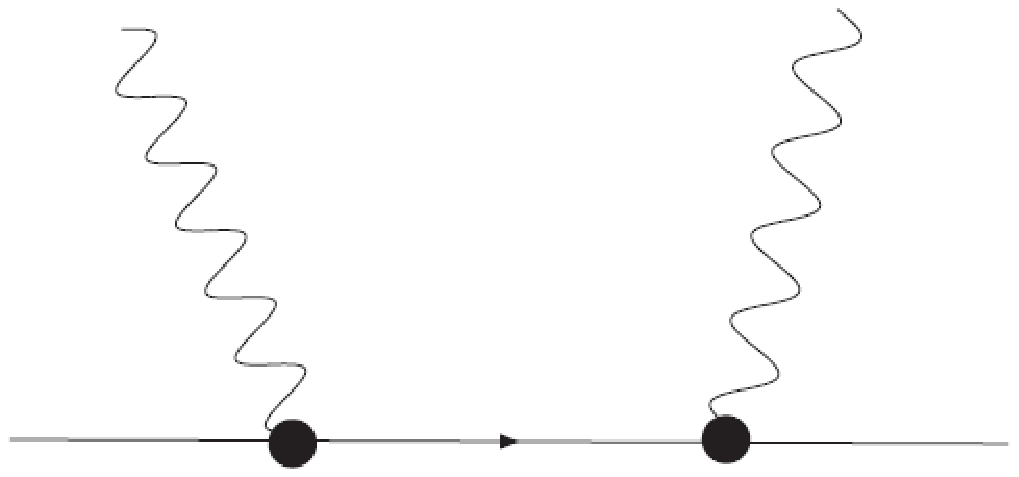
\includegraphics[width=6.5cm]{abs_cropped}
\caption{波線は$\pi$に対応し、黒い相互作用点は$\calo\pi$結合の挿入である。点を結ぶ線は、式(\ref{tfeynm})のFeynmanの時間順序積を表す。}
\label{fig1}
\end{figure}

実際、この振幅は時間順序積
\beq
\label{tfeynm}
\langle T (\delta\calo(x)\delta\calo(y))\rangle,
\eeq
に比例する。これはFeynman伝播関数$iG_{\rm F}(x-y)$とも呼ばれ、$\calL_{\rm int} = \delta\calo \pi.$をもつ通常の経路積分形式で$\delta\calo$を積分消去すると現れる。光学定理という形で表されたユニタリ性は、この振幅の虚部が単位時間当たりの全エネルギー損失と関係しなければならないことを示している\cite{dis1,dis2}。したがって、
\beq
{\rm Im}{\cal A}_{\pi\to\pi} \simeq {\rm Im}\, G_{\rm F}(\omega)
\eeq
および（$\omega>0$に対して）
\beq
\label{imgimf}
{\rm Im}\,G_{\rm F}(\omega) = {\rm Im}\,G_{\rm ret}^\calo(\omega),
\eeq
を用い、（遷移率をエネルギーに換算するため）$\omega$を掛けると、
\beq
\frac{dE}{dt} \simeq \omega{\rm Im}\,{\cal A}_{\pi\to\pi} \simeq \omega{\rm Im}G_{\rm ret}^\calo(\omega).
\eeq
を得る。この式が、$\gamma\dot\pi$という形の散逸項から従う条件
\beq \frac{dE}{dt} = \gamma \dot\pi^2, \label{dedtap}\eeq
に一致することを要求すると、予想どおり（$\omega>0$に対して）
\beq
{\rm Im}G_{\rm ret}^\calo(\omega) \simeq \gamma \omega
 \eeq
と結論される。一般には式(\ref{dedtap})はより複雑になりうるが、この手順は任意の$\omega$の関数に一般化できる\cite{dis1,dis2}。\\

読者は、遅延伝播関数ではなくFeynman伝播関数が現れることに戸惑うかもしれない。しかし、文献\cite{nrgr2,nrgr2p,nrgr2p2,radgo,eftrev}の重力放射の有効場理論（EFT）で行われているのと同様に、Feynman境界条件を用いて自己エネルギー図の虚部を全放射パワー（またはエネルギー損失）と関係づけることができる。重要なのは、$\delta\calo$の「in」状態と「out」状態が真空になるように（例えば外部からの重力放射がないように）境界条件を選ぶと同時に、全放射パワーを正確に表す虚部が生じるという点である。別の見方として、結合$\delta\calo \pi$によって誘起される全遷移率が、次の量に比例することに注目してもよい（議論を簡単にするため${\bf k}$の因子を省略する）：
\be
\sum_N    \langle \pi,0|\pi\delta\calo(t)|0,N\rangle \langle \pi,0| \pi\delta\calo(0)|0,N\rangle^\star = \sum_N  \langle 0|\delta\calo(0)|N\rangle \langle N|\delta\calo(t)|0\rangle = \langle 0| \delta\calo(0)\delta\calo(t)|0\rangle,
\ee
これは、可能なすべての（中間）状態$N$にわたる放出振幅${\cal A}_{\pi \to N}$の絶対値の二乗の和にほかならない。そこで、（$\omega>0$で成立する）関係
\beq
\int dt\, e^{i\omega t} \langle 0| \delta\calo(0)\delta\calo(t)|0\rangle = 2\,{\rm Im}\; i \int dt\, e^{i\omega t} \langle 0| T(\delta\calo(0)\delta\calo(t))|0\rangle,
\eeq
を用いると、（$\omega$を掛けた後で）先ほどの結果を再現する。これは光学定理の働きそのものである。少し微妙なのは、経路積分の方法から式(\ref{dret0})の正しい遅延境界条件をどのように得るかという点である。しかし、いわゆる「in-in」形式ではこれが可能である\cite{calzetta, weiss, Zhang}。（重力放射反作用の場合の議論については\cite{radre}を参照。）

\sectionlink{遅延Green関数} \label{appB}

この付録では遅延Green関数の基本的な性質をいくつか示し、特に、本論文全体を通じて用いた${\rm Im}G^\calo_{\rm ret} \simeq \omega$となる例を議論する。

遅延Green関数の公理的な性質から始め、空間運動量がゼロの場合を考えよう。まず、因果律から、$G_{\rm ret}^\calo(\omega)$は${\rm Im}\, \omega>0$において$\omega$の解析関数である。さらに、その虚部は$\omega$の奇関数である：
\beq
\label{prop2}
{\rm Im}\,G_{\rm ret}^\calo(-\omega)=-
{\rm Im}\,G_{\rm ret}^\calo(\omega).
\eeq
また、実部と虚部はKramers-Kronig関係によって結びついている：
\bea\label{kk}
\text{Re}\,G_{\rm ret}^\calo(\omega) & = & P \int_{-\infty}^\infty \frac{d\omega'}{\pi} \frac{\text{Im}\,G_{\rm ret}^\calo(\omega')}{\omega'-\omega}, \\
\text{Im}\,G_{\rm ret}^\calo(\omega) & = & - P \int_{-\infty}^\infty \frac{d\omega'}{\pi} \frac{\text{Re}\,G_{\rm ret}^\calo(\omega')}{\omega'-\omega},
\eea
ここで$P$は主値を表す。これより
\beq
\label{prop1}
\int_{-\infty}^{+\infty} d\omega' \frac{{\rm Im}\, G_{\rm ret}^\calo(\omega')}{\omega'} < \infty,
\eeq
が従い、さらに
\beq
{\rm Im}\,G_{\rm ret}^\calo(\omega \to 0) \to 0. \label{wtozero}
\eeq
を得る。式(\ref{wtozero})は$\omega=0$に極が存在することを禁じるが、原点から離れた領域で式(\ref{tildG})の振る舞いをすることまでは排除しない。このことは付録\ref{mag00}で示す。\\

次に、電気伝導の例を調べよう。よく知られているように、導体中の電流と電場の関係は
\beq
{\bf j}_e = -i \omega \sigma(\omega) {\bf A}(\omega),
\eeq
で与えられる。ただし${\bf E}(\omega) = -i\omega {\bf A}(\omega)$である。線形応答理論を用いると、次の式（Kubo公式）を示せる：
\beq
{\rm Re}\, \sigma(\omega) = \frac{{\rm Im}\, G^j_{\rm ret}(\omega)}{\omega},
\eeq
ここで$G^j_{\rm ret}$は電流${\bf j}_e$の遅延Green関数である。一般に、このGreen関数は\cite{forster}
\beq
G^j_{\rm ret}(\omega) = \frac{\alpha_j M_j(\omega)}{\omega + M_j(\omega)},
\eeq
とパラメータ表示できる。ここで$M_j(\omega)$は「記憶関数」、$\alpha_j$は定数である。系によっては、ある周波数域で$M_j(\omega) \sim i/\tau_j + O(\omega\tau_j)$と近似できる。$\tau_j$は「記憶時間」であり、この場合
\beq
\label{Gjret}
G^j_{\rm ret}(\omega) \simeq -\frac{\sigma_j}{i\omega-\omega_D} \quad\Rightarrow\quad {\rm Im} G^j_{\rm ret}(\omega) \simeq \frac{\sigma_j\omega}{\omega^2 + \omega_D^2},
\eeq
となる。ただし$\omega_D \simeq 1/\tau_j$、$\sigma_j = \alpha_j \omega_D$である。$\omega \ll \omega_D$では、式(\ref{drude})のDrude模型と同じ振る舞いを得る。

Re $G^j_{\rm ret} \simeq \sigma\omega_D$も成り立つことに注意されたい（これは明らかに式(\ref{kk})の分散関係と整合的である）。これは原理的にはGreen関数の実部に大きな補正が生じることを意味する。${\calo}$演算子がこの形のGreen関数をもつ場合、$\pi$に大きな質量を生じさせる可能性がある。本論文で関心をもつ場合には、近似的なシフト対称性が存在する場合のように、大きな寄与を禁じ、$m_\pi$を$O(\epsilon)$に保つ機構があると仮定した。

\sectionlink{分離極限}\label{appdec}

単一場インフレーションでは、スローロール近似のもとで$\delta N$と$\delta N_i$が抑制されることを示せる。したがって、de Sitterに\textit{近すぎない}模型では、$O(\epsilon)$の効果を除いて$\pi$の理論だけを扱えばよい\cite{eft1}。ここでは、追加自由度（ADOF）を含めても分離が成立することを論じ、混合項の構造について一般的な考察を述べる。この節では、特に断らない限り$M^2_p=1$の単位系を用いる。\\

よく知られているように、背景の全${\bar T}^{\mu\nu}$は完全流体の形
\beq
{\bar T}_{\mu\nu} = (\bar \rho_{tot}+\bar p_{tot}){\bar u}_\mu {\bar u}_\nu + \bar g_{\mu\nu} \bar p_{tot}
\eeq
をとる（これは等方性と一様性の条件から従う）。以下ではNewtonianゲージを用い、
\beq
g_{00} = -1-2\Phi,~ g_{0i}=0,~ g_{ij} = \bar g_{ij} (1-2\Psi).
\eeq
とする。

一次のスカラー摂動に注目すると、
\bea \label{stresslin}
\delta T_{ij} &=& -2\Psi \bar g_{ij} \bar p_{tot}  + \bar g_{ij} \delta p + \delta \tau_{ij}\\
\delta T_{00} &=& 2 \bar \rho_{tot} \Phi + \delta \rho \\
\delta T_{i0} &=&   - (\bar\rho_{tot}+\bar p_{tot}) \partial_i \delta u,
\eea
となる。ここにはADOFによって誘起される散逸項$ \delta \tau_{ij}$を含めた。（ADOFは$\delta\rho, \delta p$にも寄与することを忘れてはならない。）
運動方程式は\cite{weinberg}
\bea
\label{b6}
\partial_j\left(\delta p +2 \partial_0(\epsilon H^2\delta u) + 6\epsilon H^3\delta u + 2\epsilon H^2\Phi\right) +   \partial_i\delta\tau^i_j &=& 0\\
\delta\dot\rho + 3 H(\delta\rho+\delta p) + H\delta \tau^i_i + 2\epsilon H^2 \left(\frac{\nabla^2\delta u}{a^2} -3 \dot \Psi\right) &=& 0\label{b7}\\
\frac{\nabla^2\Psi}{a^2}-\frac{1}{2}\delta \rho + 3 \epsilon H^3 \delta u &=& 0\label{b8}\\
\frac{1}{a^2} \left( \partial_i\partial_j - \frac{1}{3} \delta_{ij} \nabla^2\right) (\Psi-\Phi)&=& \left(\delta\tau^i_j-\frac{1}{3}\delta_{ij} \delta\tau^l_l\right) \label{b9}
\eea
となる。ここでは$\bar \rho_{tot}+\bar p_{tot} = -2\dot H= 2H^2\epsilon$、（$\epsilon = -\dot H/H^2$）を用いた。ひとまず$\delta \rho$、$\delta p$、$\delta u$、$\delta \tau_{ij}$が計量摂動に依存しないと仮定しよう。すると、これらの方程式から、$\epsilon \to 0$の極限で計量摂動がデカップルすることが直ちにわかる。さらに、拘束方程式（最後の2式）は$\Phi$と$\Psi$を$\delta \rho$、$\delta u$、$\delta \tau_{ij}$で表す。最終的に得られる方程式では、重力との混合は$\epsilon$で抑制され、しかもこの結論は$\delta \rho$と$\delta p$の関係に依存しない。\\

これらの混合項の寄与の相対的な重要性を調べるために、式(\ref{b6} - \ref{b8})を組み合わせると、次式が得られる（$k\neq 0$）：
\bea
&&\delta\ddot \rho_k +3 H (\delta\dot\rho_k +\delta \dot p_k)-\frac{k^2}{a^2}\left(\delta p_k+ \frac{2}{3}\delta\tau_k\right)+ \frac{d}{dt}\left(H(\delta \tau^i_i)_k\right)-2\epsilon H^2 \delta\rho_k-3\epsilon H^2\delta p_k   \nn \\ && +2\epsilon H^2\delta\tau_k+10\epsilon H^2\frac{k^2}{a^2}\delta u-3\frac{a^2\epsilon H^2}{k^2}\left(\delta\ddot\rho_k + 2H \delta\dot\rho_k +4H^2\delta\rho_k\right)
+O(\epsilon^2)=0.
\eea

この式では$\partial_i (\delta \tau^i_j)_k \to 2/3~\partial_j \delta \tau_k$と置き換えた。$\delta\tau_k$は、分解$(\delta\tau^{i}_{j})^{\rm TF}_k = (\hat k^i\hat k^j-\frac{1}{3}\delta_{ij}) \delta\tau_k + \ldots$（$\hat k^2=1$）から得られるスカラーモードである。また、式(\ref{b8},~\ref{b9})を用いて$\Phi$を求めた：
\beq
\Phi = \frac{a^2}{k^2} \left(\frac{1}{2}\delta\rho_k + \delta\tau_k\right) + O(\epsilon)\label{Phid}.
\eeq

したがって、重力が存在することによる正味の効果は2つある。第一に$\sqrt{\epsilon}H$に比例する「質量」項があり、第二に地平線通過時に$\epsilon H^2/k_\star^2$程度の混合係数がある（$k_\star=k/a(t_\star)$であることを思い出そう）。よって、$\omega_\star \gg \epsilon^{1/2} H$かつ$k_\star \gg \epsilon^{1/2} H$である限り、重力との混合は無視できる。本論文の場合には$k_\star \sim \sqrt{\gamma H}/c_s > H$であるため、
\beq
{\rm mixing} \sim \frac{\epsilon_\star H_\star c_{s_\star}^2}{\gamma_\star} \ll 1 \label{mixingd}.
\eeq
に注意すると、この抑制は通常の場合よりも強いことがわかる。

これまでは、$\delta \rho$、$\delta p$、$\delta u$、$\delta \tau_{ij}$の中で計量摂動を含む項は無視できると仮定してきた。この点を明らかにするために、ADOFを含まない単一場インフレーションの例を考えよう\cite{eft1}。摂動の一次までで、式(\ref{act1})で定義された作用の最初の寄与、すなわち\footnote{$M^4_2(1+g^{00})^2$の項が$c_s\neq 1$を可能にすることに注意されたい（式(\ref{ncs})を参照）。}
\be \frac{1}{2} \int d^4 x \sqrt{-g}\{(\overline{p}-\overline{\rho}-(\overline{p}+\overline{\rho}) g^{00})+\,M_2^4 (1+ g^{00})^2\},  \ee
から得られるエネルギー運動量テンソルは、
\begin{subequations}\label{var12}
\begin{align}
\delta\rho& =\dot{\overline{\rho}}\pi+(\overline{\rho}+\overline{p}+4 M_2^4)(\dot{\pi}-\Phi), \label{rho12} \\
\delta p& =\dot{\overline{p}}\pi+(\overline{\rho}+\overline{p})(\dot{\pi}-\Phi),\\
\delta u & =-\pi.
\end{align}
\end{subequations}
を用いて式(\ref{stresslin})のように書ける。これらの変数が近似的に$\Phi$に依存しないためには、$\Phi \ll \dot\pi$である必要がある。
ADOFを含まない式(\ref{Phid})を用いて$\Phi$を解くと、（緩やかに変化する近似で、$M_p$を復元して）
\beq
\Phi\sim \frac{a^2}{M_p^2k^2}\left(\bar\rho+\bar p + 4 M_2^4\right)\dot\pi . 
\eeq
を得る。したがって、$\Phi \ll \dot\pi$という仮定は、
\beq
\label{m2ks}
\frac{a^2}{M_p^2k^2} (\bar\rho+\bar p + 4 M_2^4) \ll 1 \quad \Rightarrow\quad k_\star \gg \frac{(\bar\rho+\bar p + 4 M_2^4)^{1/2}}{M_p}.
\eeq
であれば自己無撞着である。$\bar\rho+\bar p \sim 2\epsilon M_p^2H^2$を用いると、式(\ref{mixingd})と同様の式（ただし$c_{s_\star}^2$の因子はない）を再び得る：
\beq
{\rm mixing} \sim \frac{\epsilon_\star H_\star }{\gamma_\star} \ll 1 \label{mixingd2}.
\eeq
$\epsilon \to 0$の極限では高階微分の寄与を無視できなくなるため、上の見積もりは適用できない。この場合を調べるため、式(\ref{act1})の$\bar M_2^2$に比例する項、すなわち
\beq
-\frac{1}{2}\int d^4 x \sqrt{-g}\,\bar{M}_2^2 (\delta K_{\mu}^{\mu})^2.
\eeq
を加える。$\overline{\rho}+\overline{p}\to 0$、$c_s\to 0$とすると、
\begin{subequations}
\begin{align}
\delta\rho &=4 M_2^4(\dot{\pi}-\Phi)-3\bar{M}_2^2 H\lb\frac{k^2}{a^2}\pi-3 (H\Phi+\dot{\Psi})\rb\\
&\simeq 4 M_2^4\dot{\pi}-3\bar{M}_2^2 H\frac{k^2}{a^2}\pi.
\end{align}
\end{subequations}
を得る。（第2行は、$\Phi \ll \dot{\pi}$かつ$H\Phi+\dot{\Psi}\ll \frac{k^2}{a^2}\pi$の場合に有効である。）再びADOFを含まない式(\ref{Phid})を用いると、
\beq
M_p^2\Phi\simeq \frac{a^2}{k^2}\delta\rho\simeq 4 M_2^4 \frac{a^2}{k^2}\dot{\pi}-3\bar{M}_2^2 H\pi .
\eeq
となる。したがって、$\delta\rho$の計量摂動への依存性を無視できるという仮定には、$\bar{M}_2 \ll M_p$だけでなく、次の条件も必要であることがわかる\cite{eft1}：
\be\label{mixingM2}
 M_2^4 \frac{a^2}{k^2}\ll M_p^2 \quad \to\quad k_\star  \gg M_2^2/M_p.
 \eeq
さらにこれは、式(\ref{mixingd})の混合の式がde Sitter極限で厳密にゼロになるように見えるという、一見した矛盾も説明する。（例えばゴースト凝縮では、実際にはそうならないことがわかっている。詳細については\cite{eft1}を参照。）式(\ref{mixingM2})の条件には、de Sitter極限でゼロになる$c_s$が一切現れないことに注意されたい。一般に$(\epsilon, c_s)$が小さい場合、式(\ref{m2ks})に示したように、重力との混合は$\bar\rho+\bar p$と$M_2^4$のどちらが大きいかに依存する。したがって、de Sitterに近い極限では、混合が$\epsilon$に比べて増強される可能性がある。

ADOFを含めても、上の解析は大きく変わらない。ベクトルモードとテンソルモードについても同様の議論ができる。

%---------------------------------------------------------------------------

\sectionlink{\texorpdfstring{$\hat\calo\delta K^{\mu}_{\mu}$についての考察}{Ô δKについての考察}}\label{dodk}

外部曲率を含む項の重要性を簡単に調べよう。特に、式~(\ref{extcalotr})の演算子$s(t)\frac{\hat\calo}{M_K}\delta K^{\mu}_{\mu}$を、式~(\ref{inter1n})の$f(t)\calo_1$と比較する。議論のために$\calo_1\sim\hat{\calo}$とする。これは、これらの演算子に対して、応答と雑音のすべての係数が同程度であることを意味する。このとき、$\pi$の一次では、$f(t){\calo}_1$から$\dot{f}\pi\calo_1$が得られる一方、外部曲率を含む演算子からは$\frac{s(t)}{M_{K}}\hat{\calo}\frac{\nabla^2}{a^2}\pi.$が得られる。\\

両者の比をとると、$k_\star$が
\beq \label{ksmk} k_\star^2\ll~M_{K}\dot{f}(t)/s(t), \eeq
を満たす場合には、$\delta K$を含む演算子を無視できる可能性がある。本論文で示したように、（遅延Green関数$G_{\gamma}$の振る舞いにより）パワースペクトルと非Gaussian性の計算は、凍結時に$k_\star\sim \sqrt{H\gamma}/c_s$となる値に支配される。したがって、式(\ref{ksmk})の条件を満たすためには、
\beq \frac{s(t)\gamma H}{\dot f c_s^2} \ll~M_{K}. \eeq
が必要である。そうでなければ、$\calo\delta K^{\mu}_{\mu}$からの寄与が重要となりうる。

%---------------------------------------------------------------------------

\sectionlink{膨張宇宙における散逸的Green関数}\label{greenf}

この付録では、第~\ref{nongaus}節の非Gaussian性の計算に関係するGreen関数の性質、特に$G_{\gamma}(x,y)=y^2 g_{\gamma}(x,y)$（$x=-kc_s\eta$、$y=-kc_s\eta'$）について議論する。図~\ref{GreGamma}に、$\gamma$の異なる3つの値に対する$G_{\gamma}(0,y)$のグラフを示す。（$x<(4+\gamma/H)^{1/2}$を固定すると、\footnote{$\gamma\rightarrow 0$の場合に標準的な結果を再現するため、4という因子を残している。}$G_{\gamma}(x,y)$の振る舞いは、図に示した$x=0$の場合と同様である。）$G_{\gamma}$は$y\simeq (4+\gamma/H)^{1/2}$でピークをもち、$\gamma$が増加すると振幅が減少する一方で、台は広がることがわかる。

\begin{figure}[h]
\centering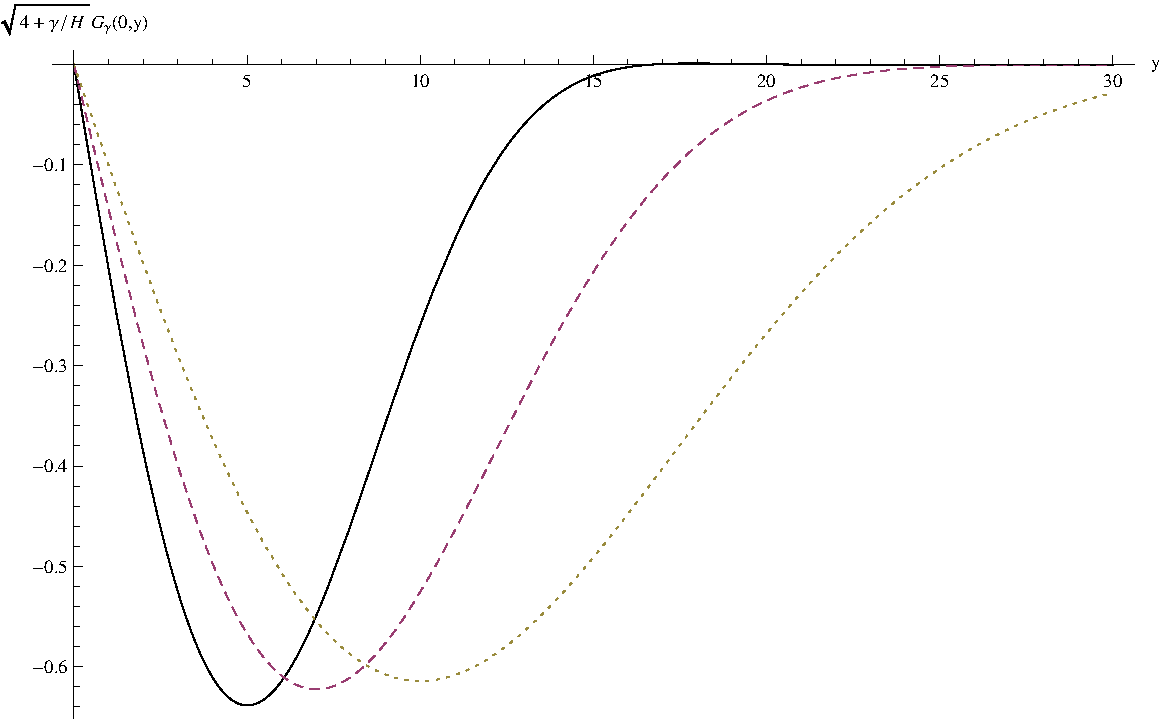
\includegraphics[width=8.5cm]{Greengamma}
\caption{$\gamma$の異なる3つの値に対するGreen関数$G_{\gamma}(0,y)=y^2 g_{\gamma}(0,y)$。$4+\gamma/H=5^2$（黒実線）、$4+\gamma/H=7^2$（破線）、$4+\gamma/H=10^2$（点線）に対し、$G_{\gamma}$の最初のピークはそれぞれ$y=5,\,7,$および$10$付近にあり、ピークの位置が$\sqrt{4+\gamma/H}$であることを裏づけている。}\label{GreGamma}
\end{figure}

\begin{figure}[h]
\centering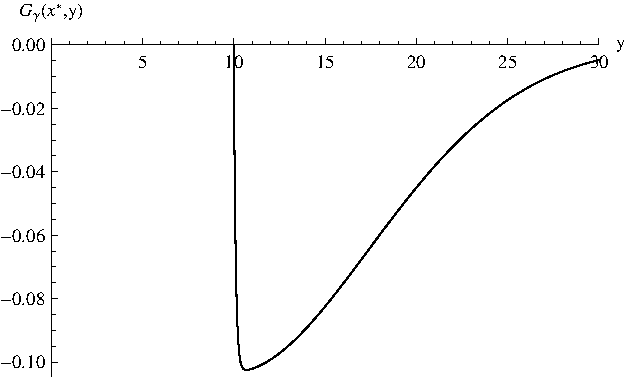
\includegraphics[width=.48\linewidth]{Greengammasqrt}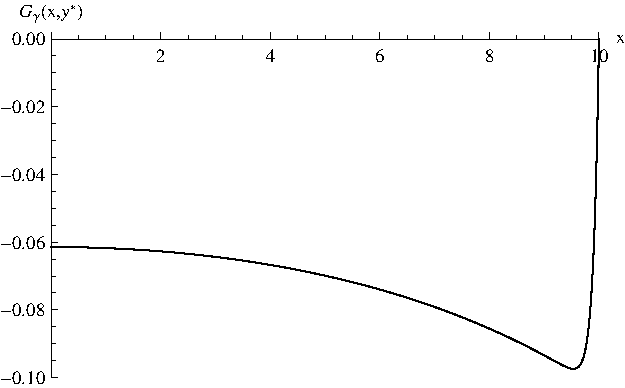
\includegraphics[width=.48\linewidth]{Greengammasqrtx}
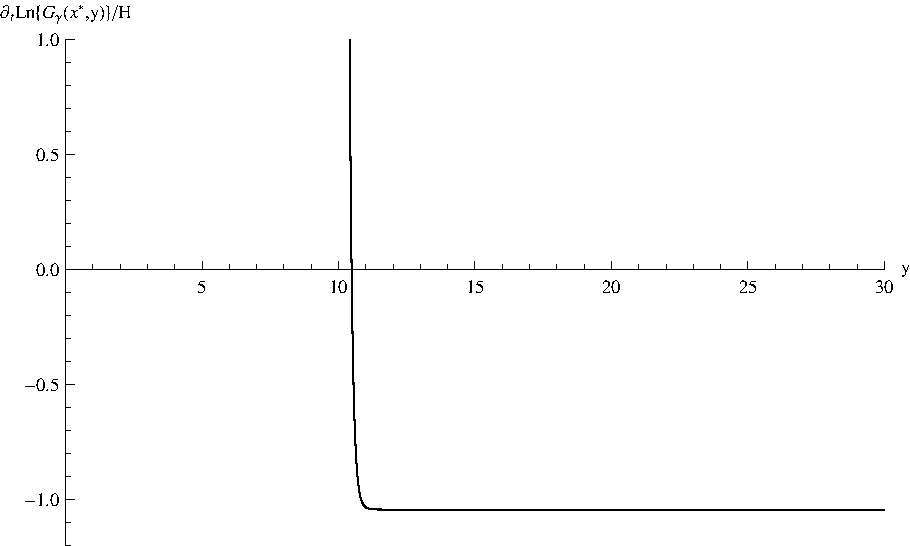
\includegraphics[width=.48\linewidth]{DotGreengammasqrt}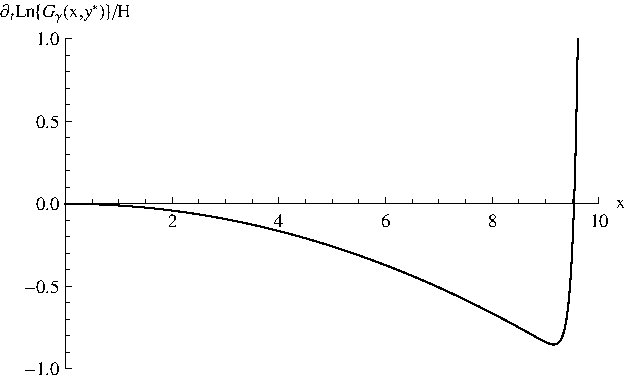
\includegraphics[width=.48\linewidth]{DotGreengammasqrtx}
\caption{Green関数$G_{\gamma}(x,y)$（上段）と、Hubble時間を単位としたその時間微分$\partial_tG_{\gamma}(x,y)/H=-x\partial_xG_{\gamma}(x,y)$（下段）。左列は$x^\star=\sqrt{4+\gamma/H}$を固定した$y>x^\star$の関数、右列は$y^\star=\sqrt{4+\gamma/H}$を固定した$x<y^\star$の関数として示す。すべての図は$x^\star=y^\star=10$に対応する。}\label{GreGamma2}
\end{figure}

ある特定の$\gamma$の値について、図~\ref{GreGamma2}にGreen関数$G_{\gamma}(x,y)$と、Hubble時間を単位としたその時間微分$\partial_tG_{\gamma}(x,y)/H=-x\partial_xG_{\gamma}(x,y)$を示した。$x=\sqrt{4+\gamma/H}$を固定して$y>x$の関数として描いたものと、$y=\sqrt{4+\gamma/H}$を固定して$x<y$の関数として描いたものを示している。$g_{\gamma}$の積分の大きさを見積もるには、
\be
\int_x^{+\infty} dy\, G_{\gamma}(x,y)=-1.
\ee
に注意すると便利である。$\gamma$が大きい場合、$y^2$の各因子を$\gamma$と数え、$G_{\gamma}$ごとに$\gamma^{-1/2}$（すなわち$g_{\gamma}$ごとに$\gamma^{-3/2}$）を、積分ごとに$\gamma^{1/2}$を掛け、$\gamma/H$を用いて単位を整えれば、$f_{\rm NL}^{\rm eq}$の大まかな見積もりが得られる。$G_{\gamma}$にHubble時間を単位とする時間微分があっても、$f_{\rm NL}^{\rm eq}$を大幅には増加させないことに注意されたい（図~\ref{GreGamma2}を参照）。一方、Hubble長を単位とする空間微分が追加されると、その寄与は$f_{\rm NL}^{\rm eq}$をおよそ$\gamma/c_s^2$倍に増加させる（$k^2/(a^2H^2)=y^2/c_s^2$であるため）。

%---------------------------------------------------------------------------

\sectionlink{混合}\label{mixing}

$\pi$の最低次における摩擦の効果を調べるために、本論文では一般的な型の演算子、すなわち$\calo\pi$の研究に集中した。ここで$\calo$には、原理的には（部分積分の後で）一連の寄与が含まれている。しかし、高次の効果を加える際には、それぞれを個別に扱った。その理由は、すべての項が同じ型の非線形性を生成するわけではないこと、そしてもちろん簡単のためでもあった。しかし一般には、複数の演算子が同時に存在する。ここでは、複数の型のADOFを同時に含めた結果として、どのような効果が現れうるかについていくつか述べる。

\subsectionlink{スカラー}\label{mixingscalars}

スカラー演算子$\calo_A$、$A=1,\ldots N$から始めよう。一般に、自己相関関数によって与えられる応答と雑音の寄与に加えて、交差相関（例えば$\langle\delta\calo^S_A\delta\calo^S_B\rangle$）による寄与も存在する。より正確には、次の形の相互作用項を考えている：
\be S_{int}=-\int d^4x a^3(t) \calo_A F^A, \ee
ここで$F^B$は、$\calo$に対応するADOFの動力学をわずかに乱す外力とみなし、繰り返された添字については和をとる。したがって、外力の印加による$\calo_A$の線形応答は
\be \delta\calo_A^R=-\int d^4x' a^3(t') G_{AB}^\calo(x,x') F^B(x'),\label{deltaO}\ee
と書ける。ここで、
\be G_{AB}^\calo(x,x')=i \theta(t-t')\langle[\delta\calo_A(x), \delta\calo_B(x')]\rangle.\ee
である。さらにADOFの揺らぎがあり、これは確率的な源$\delta\calo^S_A(x)$の2点関数によって特徴づけられる：
\be N_{AB}^\calo(x,x')= \langle\delta\calo^S_A(x)\delta\calo^S_B(x') \rangle.\ee

第~\ref{localapp}節で述べた局所近似が適用できる場合に注目すると、
\beq
\label{respoLoc}
 \delta\calo_A^R(t,{\bf k})\simeq \mu_{AB}(t) F^B(t,{\bf k})+\Gamma_{AB}(t)\frac{1}{a^{3/2}} \partial_{t}(a^{3/2}(t) F^B(t, {\bf k})),
\eeq
\beq \langle\delta{{\calo}}_A^S(t,{\bf k}_1)\delta{{\calo}}^S_B(t,{\bf k}_2)\rangle=(2\pi)^3\delta^{(3)}({\bf k}_1+{\bf k}_2)
{N}_{AB}^{\calo}(t,t'),\eeq
と書ける。ただし、
\be  {N}_{AB}^\calo(t,t')\simeq~ \nu_{AB}(t) \frac{ \delta(t-t')}{a^{3}(t)},\ee
であり、$\mu_{AB}(t),\,\Gamma_{AB}(t)$と$\nu_{AB}(t)$は近似的に時間に依存しない。

\subsectionlink{\texorpdfstring{$ f(t)\calo_1$と$\calo_2 g^{00}$}{f(t)O₁とO₂g⁰⁰}}

議論を完備させるために、前述の局所近似の仮定のもとで、$\calo_1$と$\calo_2$の混合による効果を調べよう。この混合を無視すると、相互作用$f_1\calo_1$は$\pi$の運動方程式に$\gamma\dot{\pi}$という項を与える（第\ref{ftcalo}節を参照）。一方、両演算子のGreen関数が$\omega\rightarrow 0$で${\rm Im}\,G(\omega)\propto\omega$を満たすと仮定すると、$\calo_2 g^{00}$は高階微分の寄与を生じる（第\ref{localo2}節を参照）。したがって、一次では$f_1\calo_1$の項が$f_2\delta g^{00}\calo_2$より支配的な場合を考えるのが妥当である。これにより、$\calo_2$によって導入される補正の最低次では、相互作用$\delta g^{00}\calo_2$単独からの寄与を無視でき、その効果が$\calo_1$との混合のみを通じて現れる状況に注目できる。例えば、$\calo_1=\calo_2$かつ$f_2 H\ll\dot{f_1}$であればこの場合に該当する。したがって実際には$f_2$の最低次で計算できる。さらに簡単のため、ここでは線形応答近似を用いて得られる寄与だけに注目する。ただし、第\ref{localo2}節で見たように、$ f_1\calo_1$から得られる非線形応答の寄与が、この種の模型で最大の非Gaussian性を生成する可能性がある\footnote{第\ref{ftcalo}節の解析から、相互作用$f_1\calo_1$だけが存在する場合、線形応答近似の範囲で得られる非Gaussian性は無視できるほど小さいことに注意されたい。}。

混合による応答項には2つの型がある。一方は$f_1(t)$（$\calo_1$に結合する力）が$\delta\calo_2$に及ぼす影響によるものであり、もう一方は$f_2\delta g^{00}$が$\delta\calo_1$に及ぼす影響によるものである。局所近似を用いると、これらは
\begin{subequations}
\begin{align}
\delta\calo_1^{R_{\rm mix}}&\simeq~ -f_2\tilde{\mu}_{12}\lp 2\dot{\pi}+\dot{\pi}^2-\frac{\partial_i\pi\partial_i\pi}{a^2}\rp\nonumber\\
&-f_2\Gamma_{12}\lp2\ddot{\pi}+2\dot{\pi}\ddot{\pi}-2\frac{\partial_i\pi\partial_i\dot{\pi}}{a^2}+2H\frac{\partial_i\pi\partial_i\pi}{a^2}\rp,\\
\delta\calo_2^{R_{\rm mix}}&\simeq~ \tilde\mu_{21}\lp\dot{f_1}\pi+\ddot{f_1}\frac{\pi^2}{2}\rp+\Gamma_{21}\lp\dot{f_1} \dot{\pi}+\ddot{f_1}\dot{\pi}\pi\rp,
\end{align}
\end{subequations}
と書ける。ここで$\tilde{\mu}_{AB}={\mu}_{AB}+3/2H\Gamma_{AB}$であり、本文で述べたような創発的シフト対称性が存在すると仮定した。

$f_2$の一次までで、$\pi_1$の方程式は
\be
\ddot{\pi}_1+(3H+\tilde{\gamma})\dot{\pi}_1+\tilde{c}_s^2\frac{\nabla^2}{a^2}\pi_1=-\tilde{N}_c^{-1}
\left(\dot{f_1}\delta\calo_1^S-2f_2\frac{\partial_t(a^3\delta\calo_2^S)}{a^3}\right),
\ee
となる。ここで$\tilde{N}_c=N_c+2f_2\dot{f_1}(\Gamma_{21}-\Gamma_{12}))$、$\tilde{c}_s^2={c}_s^2-2f_2\tilde{N}_c^{-1}\dot{f_1}c_s^2(\Gamma_{21}-\Gamma_{12})$、$\tilde{\gamma}= \tilde{N}_c^{-1}\left(\dot{f_1}^2\Gamma_{11}+2f_2\dot{f_1}(3H\Gamma_{12}-\tilde{\mu}_{12})\right)$である。$\tilde{c}_s^2\tilde{N}_c=c_s^2N_c $が成り立つことに注意されたい（$f_2$の一次までで計算していることを思い出そう）。記法を簡単にするため、以下ではチルダを省略する。上の方程式の特解は
\begin{eqnarray}
\pi_1(k,\eta)&=&\frac{\dot{f_1} k c_s}{N_cH^2}\int^{\eta}_{\eta_0} d\eta'g_{\gamma}(kc_s|\eta|,kc_s|\eta'|)\delta\calo_1^S({\bf k},\eta')\nonumber\\
&+&\frac{2 f_2 k c_s}{N_cH^2}\int^{\eta}_{\eta_0} d\eta'g_{\gamma}(kc_s|\eta|,kc_s|\eta'|)\frac{\partial_t \lp a^3(\eta')\delta\calo_2^S({\bf k},\eta')\rp}{a^3(\eta')},
\end{eqnarray}
であり、得られるパワースペクトルは
\be
P_{\zeta}=P_{\zeta}^{f_2=0}\lp 1+6\frac{H f_2\nu_{12}} {\dot{f_1}\nu_{11}}\rp
\ee
と書ける。$P_{\zeta}^{f_2=0}$は$f_2=0$で得られるものであり、式~(\ref{pow1gamma})で$\nu_\calo=\nu_{11}\dot{f_1}^2$としたものである。$\pi$に対する源は
\begin{eqnarray}
J&=&N_c^{-1}\dot{f_1}(2f_2H\Gamma_{12}-f_2\tilde{\mu}_{12}) \frac{\partial_i\pi\partial_i{\pi}}{a^2}-2N_c^{-1} f_2\dot{f_1}(\Gamma_{12}-\Gamma_{21})\frac{\partial_i\pi\partial_i\dot{\pi}}{a^2}\nonumber\\
&+&2f_2N_c^{-1}\dot{f_1}\Gamma_{21} \dot{\pi}\frac{\nabla^2\pi}{a^2}+f_2N_c^{-1}\dot{f_1}(\tilde{\mu}_{12}-6H\Gamma_{21})\dot{\pi}^2+2f_2N_c^{-1}\dot{f_1}(\Gamma_{12}-2\Gamma_{21})\dot{\pi}\ddot{\pi}\nonumber\\
&-&\dot{f_1}\delta\calo_1^S-2f_2\frac{\partial_t\lp a^3\delta\calo_2^S\rp}{a^3}-2f_2\frac{\partial_t\lp a^3\dot{\pi}\delta\calo_2^S\rp}{a^3}+2f_2N_c^{-1}\frac{\partial_i\lp\delta\calo_2^S\partial_i\pi\rp}{a^2}.\label{mixsource}
\end{eqnarray}
となる。$\calo_1=\calo_2$なら第2項は消えることに注意されたい。\\

第\ref{nongaus}節の計算からわかったように、非Gaussian性を生成するうえでは、空間微分をもつ非線形項の寄与が、時間微分だけをもつ項の寄与よりも重要となる。そこで簡単のため、主要な項に含まれると予想される最初と最後の項だけを調べよう。最初の源の項についての計算は、第\ref{Nolocalo2}節で式~(\ref{pieqnl})の右辺第1項に対してすでに行った計算とまったく同じである。実際、これは
\be J_k^1=-s_1\gamma\frac{\partial_i\pi\partial_i{\pi}}{a^2},\ee
と書ける。ただし、
\be
s_1=-\frac{2f_2 H}{\dot{f_1}}\frac{\Gamma_{12}}{\Gamma_{11}} +\frac{f_2\tilde{\mu}_{12}} {\dot{f_1}\Gamma_{11}}, \ee
である。簡単のため$\gamma_{AB}\sim H \mu_{AB}$とすると、$f_2$についての線形展開と整合するように$s_1\ll 1$となる。式~(\ref{fnlgoonoloc})から
\beq f_{\rm NL}^{\rm eq}\simeq\frac{s_1\gamma}{2H c_s^2},\eeq
を得る。$c_s\lesssim 1$であり、近似が有効な範囲、すなわち$s_1 \ll 1$であっても、$\gamma\gg H$であればこれは依然として大きくなりうる。\\

同様に、源の最後の項については
\begin{eqnarray}
f_{\rm NL}^{\rm eq}&=&-\frac{10}{3}\frac{s_2}{c_s^2}\frac{2^{-8\gamma/H}\pi^2 {\Gamma\left(\frac{2\gamma}{H}+4\right)}^2}{\lp\frac{\gamma}{H}+1\rp^6{\Gamma\lp\frac{\gamma+H}{2 H}\rp}^8}
 \int_{0}^{+\infty} dy' {y'}^6 (g_{\gamma}(0, y'))^2\nonumber\\&\times&\int_{y'}^{+\infty} dz z^4  g_{\gamma}( y',z)g_{\gamma}(0, z),\label{fnlmix2n}
\end{eqnarray}
を得る。ここで$s_2=\frac{f_2H}{\dot{f_1}}\frac{\nu_{12}}{\nu_{11}}\ll 1$であり、再び簡単のため、すべての質量スケールは同程度とした。数値計算を行うと、$\gamma/H\gg 1$の領域では$f_{\rm NL}$を
\beq
f_{\rm NL}^{\rm eq}\simeq- 3\frac{\gamma}{H} \frac{s_2}{ c_s^2},
\eeq
によってよく近似でき、前の場合と同様の結果となる。

\subsectionlink{ベクトルとテンソル}\label{vectens}

最後に、第\ref{vectors}節および第\ref{tensors}節で論じたように、追加できる一群のベクトルおよびテンソル相互作用項がある。これらは
\begin{eqnarray}\label{family}
S^{\calo}&=&-\int d^4 x \sqrt{-g}\,\left(f_1(t)\calo^{0}_1+f_2(t)\calo^{00}_2+f_3(t)\calo^{000}_3+\ldots\right) \\
&-&\delta g^{00}\left(s_1(t)\calo^{0}_1+s_2(t)\calo^{00}_2+s_3(t)\calo^{000}_3+\ldots\right)+\ldots\nonumber
\end{eqnarray}
と書ける。

議論と記法を簡単にするため、ここでは、一般にその時間依存性がスローロールで抑制される因子$f_i(t)$と$s_i(t)$を省略しよう。\\

$\pi$を導入すると、これらの項は
\begin{subequations}\begin{align}
\calo^{0}_1&=\calo^{\mu}_1\partial_{\mu}(\tilde{t}+\pi)=\calo^{0}_1+\calo^{\mu}_1\partial_{\mu}\pi\\
\calo^{00}_2&=\calo^{\mu\nu}_2\partial_{\mu}(\tilde{t}+\pi)\partial_{\nu}(\tilde{t}+\pi)\\&=\calo^{00}_2+2\calo^{0\mu}_2\partial_{\mu}\pi+\calo^{\mu\nu}_2\partial_{\mu}\pi\partial_{\nu}\pi\nonumber\\
\calo^{000}_3&=\calo^{\mu\nu\rho}_3\partial_{\mu}(\tilde{t}+\pi)\partial_{\nu}(\tilde{t}+\pi)\partial_{\rho}(\tilde{t}+\pi)\\&=\calo^{000}_3+3\calo^{00\mu}_3\partial_{\mu}\pi+3\calo^{0\mu\nu}_3\partial_{\mu}\pi\partial_{\nu}\pi+\calo^{\mu\nu\rho}_3\partial_{\mu}\pi\partial_{\nu}\pi\partial_{\rho}\pi,\nonumber
\end{align}
\end{subequations}
などとなる。これらをすべて足し合わせると、
\be\label{suma}
\calo^{0}_1+\calo^{00}_2+\calo^{00}_3+\ldots=\tilde{\calo}+\tilde{\calo}^{\mu}\partial_{\mu}\pi+\tilde{\calo}^{\mu\nu}\partial_{\mu}\pi\partial_{\nu}\pi+\tilde{\calo}^{\mu\nu\rho}\partial_{\mu}\pi\partial_{\nu}\pi\partial_{\rho}\pi \ldots,
\ee
を得る。$\tilde \calo^{\mu\ldots\nu}$は、もとのテンソル演算子の何らかの組み合わせから構成される。式~(\ref{family})の第2行も同様に並べ替えることができる。\\

例として、式~(\ref{suma})の最初の$\pi$に依存する項を生成する$\calo^0 \equiv \calo_\mu g^{\mu0}$を考えよう。式を見ればわかるように、$\pi$の一次では、この演算子の解析は、本論文を通して調べてきたスカラー演算子の解析へと帰着できる。実際、部分積分すると、
\beq \label{oeff} \int d^4x \sqrt{-g} \calo^\mu \partial_\mu \pi \to \int d^4x \left(\partial_\mu \sqrt{-g} \calo^\mu\right)\pi \equiv \int d^4x \sqrt{-g} \tilde\calo \pi,
\eeq
を得る。ここで$\tilde\calo= \frac{1}{\sqrt{-g}}\partial_{\mu}(\sqrt{-g}{\calo}^{\mu})$は有効スカラー演算子である。この相互作用は構成のしかたからシフト対称性を満たす。さらに、第\ref{localapp}節の仮定を満たすならば、$\gamma \gg H$に対して大きな摩擦項を誘起しうるが、作用中には$O(\pi^2)$の項が生じない。素朴には、この場合には摩擦と非Gaussian性に関係がないように思えるかもしれない。しかし、本論文全体を通じて強調したように、非線形応答は非線形結合を誘起する。これらは実際に大きいと予想され、$f_{\rm NL} \simeq\gamma/c_s^2H$を与える。

%-------------------------------------------

\sectionlink{\texorpdfstring{$\gamma\dot\pi$型の散逸を伴う$\calo\delta g^{00}$模型}{γ π̇型の散逸を伴うO δg⁰⁰模型}}\label{mag00}

この付録では、$\gamma\dot\pi$型の散逸を伴う$\tilde\calo g^{00}$型の結合の例を議論する。第\ref{storyo}節で論じたように、これには特殊な解析構造が必要であり、特に、間もなく定める周波数域$\mu_\calo < \omega < \Gamma_\calo$において（式(\ref{tildG})を参照）、
\beq
{\rm Im} \tilde G_{\rm ret}^\calo (\omega) \sim 1/\omega,
\eeq
が必要となる。ここでは、インフラトンを、$\pi$とは直接結合しない第2の（隠れた）セクターによって強い散逸的動力学を与えられるスカラー場に結合させる、一つの可能な模型を導入する。この設定については別の機会にさらに詳しく調べる予定である。（以後はチルダを省略し、また多数の$\gamma$が現れるため、$\pi$の散逸係数を$\gamma_\pi$と表す。）\\

基本的な考え方は文献\cite{eft1}のインフレーションのEFTを用いることである。ただし、文献\cite{dan2}の模型と同じ考えに基づき、$\sigma \delta g^{00}$という項を通じて$\pi$をスカラー場$\sigma$に結合させ、質量の単位をもつ$\rho$を係数とする$\rho \sigma\dot\pi$結合を生成する\cite{dan2}。その動力学を
\beq
\calL_\sigma = \frac{1}{2}(\partial_\mu \sigma)^2 - \frac{1}{2} \mu^2 \sigma^2 + \sigma J_\Psi,
\eeq
と書く。ここで$J_\Psi$は、$\sigma$と、まとめて$\Psi$と表される散逸セクターとの相互作用を表す。このセクターは$\pi$とは直接結合しない。\footnote{原理的には$\Psi$は重力相互作用を通じてインフラトンと相互作用しうるが、それらは劣勢の寄与である。}本質的には、これは$\pi$が混合項を介して散逸する2段階の模型である。文献\cite{multieft}の枠組みでも記述できるが、ここではさらに、$\sigma$に結合して（強い）散逸を誘起するセクターが存在する。（例えば、$\Psi$系をある温度$T_\Psi$の熱平衡状態に置いてもよい。）\\

ここで$\sigma$の遅延Green関数を計算すると、次式を得る（図\ref{odot}を参照）：
\beq
\rho^2 G^\sigma_{\rm ret}(\omega,{\bf k}) = \frac{\rho^2}{\omega^2-{\bf k}^2 - \mu^2 + \Gamma_\Psi(\omega)},
\eeq
ここで$\Gamma_\Psi$は、$\sigma J_\Psi $結合による$\langle[ J_\psi, J_\psi] \rangle$相関関数からの自己エネルギー寄与である（後述）。この自己エネルギーの虚部を
\beq
\label{imsigm}
{\rm Im}\, \Gamma_\Psi(\omega) \simeq \gamma_\Psi \frac{\omega}{\omega+\Lambda_\psi},
\eeq
と近似できると仮定しよう。これはより標準的な振る舞い（式(\ref{drude})のDrude模型に類似）であり、$\omega < \Lambda_\psi$では$\omega$に対して線形に振る舞う。付録\ref{appB}を参照されたい。上半平面における$\Gamma_\Psi$の解析性を用いると、（Kramers-Kronig関係を通じて）$\omega \lesssim \Lambda_\Psi$に対し
\beq
\label{resigm}
{\rm Re}\,\Gamma_\Psi(\omega) \simeq \gamma_\Psi \Lambda_\Psi \left(\frac{\Lambda_\Psi^2}{\omega^2+\Lambda_\Psi^2}\right) \simeq \gamma_\Psi \Lambda_\Psi,
\eeq
も得られる。したがって、
\beq
\label{imGs}
\rho^2 {\rm Im}\, G^\sigma_{\rm ret}(\omega,{\bf k}) \simeq  \frac{\gamma_\Psi \rho^2 \omega}{\left[\omega^2-{\bf k}^2 - \mu^2 + \gamma_\Psi \Lambda_\Psi \right]^2 + \gamma_\Psi^2\omega^2}.
\eeq

\begin{figure}[h!]
\centering
    \centering
    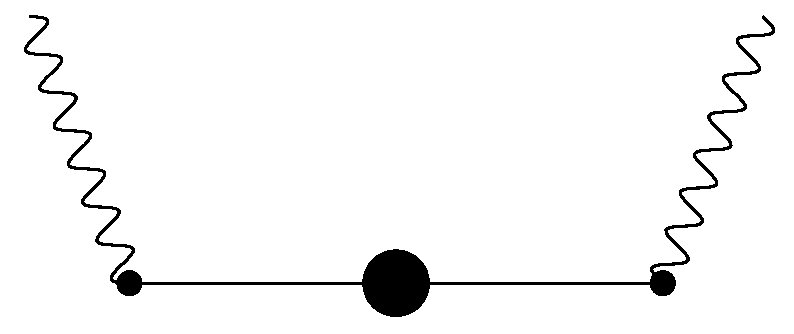
\includegraphics[width=6.5cm]{odotfig_cropped}
\caption{波線は$\pi$に対応し、黒い相互作用点は$\sigma\dot\pi$結合の挿入である。大きな黒丸は、$\sigma J_\Psi $結合から生じる$\langle [J_\psi, J_\psi]\rangle$相関関数のGreen関数を表す。}
\label{odot}
\end{figure}

ここで求めたいのは、運動方程式に$\gamma_\pi \dot\pi_k$が得られる領域、言い換えると、式(\ref{tildG})のスケーリングが式(\ref{imGs})で実現する領域である。これは実際、
\beq
\label{mutuned2}
\left[\omega^2-{\bf k}^2 - \mu^2 + \gamma_\Psi \Lambda_\Psi \right]^2 \ll \gamma_\Psi^2\omega^2.
\eeq
の場合に実現する。

$\omega\lesssim \Lambda_\Psi$という制約を考えると、素朴にはこれを実現するのは難しそうに見える。しかし、大きな寄与を打ち消すように$\mu$を設定することは常に可能である。例えば、\footnote{（保護されていない）スカラー場を扱う際に、ある程度の微調整が必要になることは驚くべきことではない。一つの可能性は、$\sigma$を擬Goldstoneボソンとみなすこと、あるいは対称性の破れのスケールをHubbleスケール付近とした超対称な版を導入することである。（その意味で、これは文献\cite{multieft}の超対称多場インフレーションのEFTに似ている。文献\cite{dan2new}も参照。）この問題は今後の課題として残す。}
\beq
\label{mutuned}
\gamma_\Psi \Lambda_\Psi - \mu^2 \simeq H^2.
\eeq
と調整すればよい。さらに$\omega_\star, k_\star \ll \gamma_\Psi$も仮定する（これは自己無撞着であることを後に示す）。すると、採用した仮定のもとで、$H \lesssim  \omega, |{\bf k}| \lesssim \gamma_\Psi (\lesssim \Lambda_\Psi)$に対し
\beq
\label{imGs2}
\rho^2 {\rm Im}\, G^\sigma_{\rm ret}(\omega) \simeq  \frac{\gamma_\Psi \rho^2}{\gamma_\Psi^2}\frac{1}{\omega},
\eeq
を得る。したがって、
\beq
\gamma_\pi \sim \frac{\rho^2}{\gamma_\Psi},
\eeq
であり、$\rho \sim \gamma_\Psi$の場合には$\gamma_\pi \sim \gamma_\Psi$となる。本論文で示したように、$\gamma_\pi\dot\pi$という散逸項がある場合には$k_\star \simeq \sqrt{\gamma_\pi H}$となるため、$\gamma_\pi \gg H$であれば式(\ref{imGs2})を導いた条件は満たされる。\\

パワースペクトルと非Gaussian性を計算するためには、雑音部分も必要である。これもまた、$\sigma$を介した$\pi$と$J_\Psi$の（間接的な）結合から従う。このことは、運動方程式を明示的に書けば示せる（簡単のためHubble膨張を無視する）：
\bea
\label{ddpis}\ddot\pi_k + k_{\rm ph}^2\pi_k &=& -\rho\dot\sigma_k, \\
\label{ddsig}\ddot\sigma_k + (k_{\rm ph}^2+\mu^2)\sigma_k &=& J_\Psi + \rho\dot\pi_k.
\eea

上で論じたように、関心のある領域では（$J_\Psi$を特定の演算子~$\delta\calo$とみなして）、
\beq
J_\Psi =  J^S_\Psi + \int G^\Psi_{\rm ret} \sigma \simeq J^S_\Psi +\gamma_\Psi\Lambda_\Psi\sigma - \gamma_\Psi\dot\sigma,
\eeq
と書ける。ここでは式(\ref{imsigm})および(\ref{resigm})を用い、先ほどと同様に確率的な源の項$J^S_\Psi$を加えた。したがって、式(\ref{mutuned2})に従って$\mu$を選ぶと、
\beq
 \gamma_\Psi\dot\sigma_k \simeq \rho\dot \pi_k - J^S_\Psi,
\eeq
となり、これを式(\ref{ddpis})に代入すると最終的に
\beq
\ddot\pi_k + k_{\rm ph}^2\pi_k +\gamma_\pi \dot\pi_k = J^S_\pi,
\eeq
を得る。ただし$J^S_\pi =\left(\rho/\gamma_\Psi\right) J^S_\psi$である。このように式(\ref{eom1})と同じ形の方程式が残り、本論文を通じて行った計算が適用できる。特に、第~\ref{Nolocalo2}節と同様に$f_{\rm NL} \simeq \gamma_\pi/(c_s^2 H)$程度の非Gaussian性を得る。\\

$\sigma$をゲージ結合$g A^\mu \partial_\mu \pi$に置き換えることで、${\calo}_\mu g^{\mu0}$型の演算子についても同様の模型を構成できることに注意されたい。その場合、$J_\Psi$は通常の電磁電流と同様の役割を果たす（付録\ref{appB}を参照）。

\sectionlink{局所的なトラップ型インフレーションの整合性}\label{consistency}

ここでは、近似の妥当性を保証する基本的な制約をいくつかまとめる。背景方程式については、
\be\label{c5c6} |\ddot{\phi}|\ll 3H|\dot{\phi}|\ll V'(\phi),\ee
が必要であり、このとき等速度の解
 \be\label{E1} \dot{\phi}\simeq~ -\frac{(\Gamma_\chi|\Delta|(2\pi)^3 V')^{2/5}}{g}.\ee
が得られる。さらに、エネルギー密度はポテンシャルエネルギーに支配されると仮定する：
\be\label{EnDens} 3M_p^2 H^2=\frac{\dot{\phi}^2}{2}+V(\phi)+\sum_i M_{\chi_i} n_{\chi_i}\simeq V(\phi).\ee
一般化されたスローロールパラメータ$\epsilon=-\dot{H}/H^2$は、
\be\epsilon=\frac{3(\dot{\phi}^2+\sum_i M_{\chi_i} n_{\chi_i})}{2 V(\phi)}.\ee
で与えられる。したがって、$\epsilon\ll 1$から
\begin{subequations}\begin{align}
&\dot{\phi}^2\ll V(\phi),\label{c7}\\
&\sum_i M_{\chi_i} n_{\chi_i}\ll V(\phi),\label{c8}
\end{align}\end{subequations}
が従う。これらは式(\ref{EnDens})の近似に必要な条件である。式(\ref{c8})の左辺を見積もるため、上と同様に和を積分に置き換えると、
\be
\sum_i M_{\chi_i} n_{\chi_i}\simeq~\frac{g^{5/2}|\dot{\phi}|^{7/2}}
{\Gamma_{\chi}^2|\Delta|(2\pi)^3}\ll V(\phi).
\ee
を得る。すべての条件をまとめると、式(\ref{c1})、(\ref{c2n})、(\ref{c3c4})、(\ref{c5c6})、(\ref{c7})、(\ref{c8})に加えて、$k_{\rm ph} \ll \kappa$、$k_{\rm ph}\Delta \ll |\dot \phi|$、さらに$\Gamma_\chi\gg H$という条件がある。また、e-fold数についても
\be \label{efolds}N_e=\int \frac{H}{\dot{\phi}}d\phi=\frac{5 g m \phi ^2}{16 2^{7/10} \sqrt{3} \pi ^{6/5} \left(m^2 \Gamma_\chi  \Delta  \phi \right)^{2/5}},\ee
を得る。ここでは$\phi\equiv\phi_I \gg\phi_E$を用いており、$\phi_I$（$\phi_E$）はインフレーションの開始時（終了時）におけるインフラトン場の値である。

\begin{figure}[h!]
\centering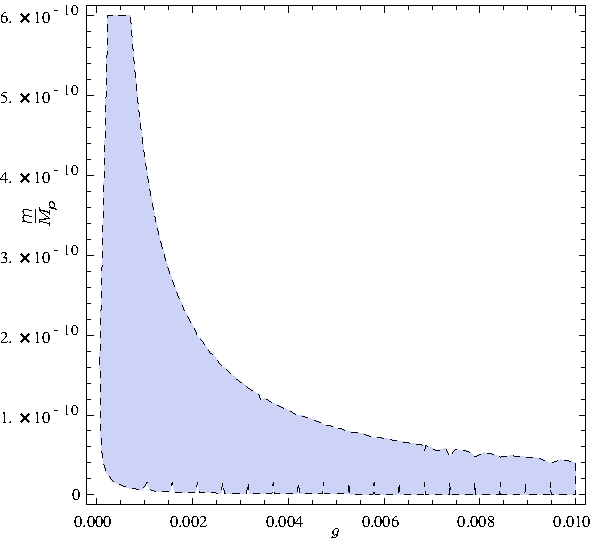
\includegraphics[width=.48\linewidth]{TrapdecayCuadgama100HFin}
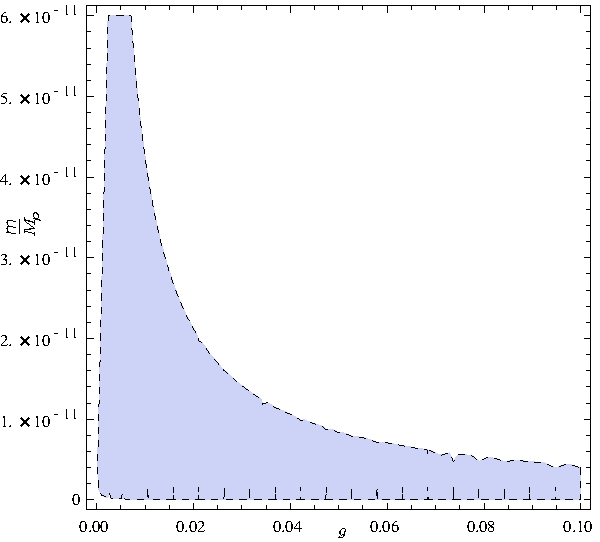
\includegraphics[width=.48\linewidth]{TrapdecayCuadgama1000HFin}
\caption{整合性によって許される自由パラメータ（$m$と$g$）の領域（$``\ll"$を$``<"$に置き換えた）。横軸は$g$、縦軸は$m/M_p$を表す。左：$\Gamma_\chi=100 H$（場合I）、右：$\Gamma_\chi=1000 H$（場合II）。}
\label{RR}
\end{figure}

次に、代表的な例である
\be V(\phi)=\frac{m^2}{2}\phi^2.\ee
について、これらの制約を調べる。

この模型には、$m,\,\Delta,\,\Gamma_\chi,\,g$と、インフラトン場の初期値$\phi_I$の5つのパラメータがある。パラメータ空間を縮小するため、$N_e=60$および
\beq
P_{\zeta}\simeq\lp\frac{H}{\dot{\phi}}\rp^2P_{\delta\phi}\simeq \frac{10^{-9}}{k^3},
\eeq
を課す。これより、次の条件を得る（式(\ref{zeta2nu})を参照し、$N_c \simeq \dot\phi^2$を用いる）：
\beq\label{E2}
\lp\frac{H}{\dot{\phi}}\rp^2 \frac{g^2\nu_{\chi}}{4}\lp\frac{\pi H}{\gamma}\rp^{1/2}\simeq 10^{-9}.
\eeq
すると、
\begin{equation}\phi \simeq \frac{16 2^{3/16} 3^{15/16} \pi ^{3/4} \sqrt[4]{\Gamma_\chi  |\Delta| }}{\sqrt[8]{g^5 m}} M_p,~~
|\Delta|\simeq\frac{1179648\times 10^{34} \sqrt[4]{6} \pi ^{11} g^{13/2} m^{9/2} M_p}{\Gamma_\chi }
\end{equation}
となる。簡単のため、$\Gamma_\chi=100 H$（場合I）と$\Gamma_\chi=1000 H$（場合II）の2つの場合を調べる。図~\ref{RR}には、すべての条件を満たすパラメータ$m$と$g$の2次元領域を示した（$``\ll"$を$``<"$に置き換えた）。横軸は$g$、縦軸は$m/M_p$を表し、場合Iが左のグラフ、場合IIが右のグラフに対応する。例として$\Gamma_\chi=100 H$、$m=10^{-11}M_p$、$g= 10^{-2}$とすると、$H\simeq 1.3\times 10^{-11} M_p$、$\gamma/H\simeq  135$、$\phi\simeq 3.3 M_p$、$\delta t_c \simeq 1.98 \times 10^{-4} H^{-1}$、$|\Delta|\simeq 1.29\times 10^{-8}M_p$、$\epsilon\simeq 1/32$を得る。また、$\Gamma_\chi=1000 H$、$m=5\times 10^{-13}M_p$、$g= 10^{-1} $に対しては、$H\simeq 3.34\times 10^{-13} M_p$、$\gamma/H\simeq 539$、$\phi\simeq 1.63 M_p$、$\delta t_c \simeq 1.4\times 10^{-5} H^{-1}$、$|\Delta|\simeq 2.27\times 10^{-7} M_p$、$\epsilon\simeq 1/32$を得る。すべての場合に$\gamma/H \ll g|\dot\phi|/H^2$であり、これは局所近似$k_\star\lesssim \kappa$の妥当性を保証する。最後の確認として、理論に追加したスカラー自由度の揺らぎから生じる曲率摂動の大きさを見積もろう。文献\cite{trapped}に従い、この寄与は
\beq
M_p^2\frac{\partial_i^2}{a^2} \delta g_\chi \sim M_\chi \Delta n_\chi,
\eeq
を計算することによって見積もれる。ここでは$M_\chi(\delta t_c) \simeq g |\dot\phi| \delta t_c \simeq \sqrt{g|\dot\phi|}$とする。上式の$\delta g_\chi$は曲率摂動$\zeta_\chi$そのものではないが、それでも誘起される曲率の大きさの目安を与える。比較のため、この式を$k/a \simeq H$で評価すると、
\beq
\langle\delta g_\chi\delta g_\chi\rangle \simeq \frac{(g|\dot\phi|)^{5/2}N_{\rm hits}}{HM_p^4}.
\eeq
を得る。一方、第\ref{power}節の解析から（式(\ref{nunhits})を参照）、
\beq
\langle\zeta_\phi\zeta_\phi\rangle \simeq \sqrt{H/\gamma} \frac{H^2}{\dot\phi^2} \frac{g^2(g|\dot\phi|)^{3/2}N_{\rm hits}}{\Gamma_\chi}.
\eeq
が得られる。したがって、$\dot\phi^2 \sim \epsilon_\phi V$（$\epsilon_\phi < \epsilon$）を用いると、
\beq
 \frac{\langle\delta g_\chi\delta g_\chi\rangle}{\langle\zeta_\phi\zeta_\phi\rangle} \simeq \frac{\Gamma_\chi k_\star}{M_\chi^2} \epsilon_\phi^2 \ll 1,\eeq
となる。これは$\Gamma_\chi\lesssim M_\chi\,, k_\star\lesssim M_\star$かつ$\epsilon_\phi\lesssim 1$であるためである。したがって、これらの曲率摂動は劣勢となる。





\clearpage
\renewcommand{\refname}{\hyperlink{toc}{参考文献}}
\bibliographystyle{utphys}
\bibliography{ref}
\end{document}
